%%%%%%%%%%%%%%%%%%%%%%%%%%%%%%%%%%%%%%%%%%%%%%%
% PREAMBLE %%%%%%%%%%%%%%%%%%%%%%%%%%%%%%%%%%%%
%%%%%%%%%%%%%%%%%%%%%%%%%%%%%%%%%%%%%%%%%%%%%%%

% Declare document (& font size)
\documentclass[11pt]{article}

% Title & other meta-data
\title{Understanding is Compression, Problem-Solving is Search, Intuition is Pattern-Matching}
\author{Nicky Case and Nora Danger}

% Useful packages
\usepackage{amsmath}       % math symbols & equations
\usepackage{graphicx}      % \includegraphics for images
\usepackage[english]{babel} % language-specific typesetting (hyphenation, etc.)
\usepackage[T1]{fontenc}   % proper encoding for accented characters
\usepackage{stfloats}      % fixes bottom floats in two-column layout
\usepackage{comment}       % for block comments
\usepackage{microtype}     % Nicer typography
\usepackage[bottom]{footmisc} % keep footnotes at page bottom
\usepackage{multicol}      % multiple columns (used for ToC)
\usepackage{palatino}      % nice font
\usepackage{caption}       % captionof
\usepackage{float}
\usepackage[normalem]{ulem} % strikeout

% Don't break words!
\usepackage[none]{hyphenat}
\emergencystretch=2em % and don't fuck shit up (\sloppy is too severe)
% but DO break them if hyphens!
\tolerance=9999
\hyphenpenalty=10000
\exhyphenpenalty=0

% Footnotes at bottom, no indent
\makeatletter
\renewcommand\@makefntext[1]{\noindent\makebox[8pt][r]{\@thefnmark.\,}#1}
\makeatother

% Not eye-bleeding blue links
\usepackage{xcolor} % custom colors (used for link color)
\usepackage[most]{tcolorbox} % boxes (cite box)
\definecolor{linkblue}{RGB}{50, 80, 170}
\usepackage{xurl} % lets long URLs break anywhere
\usepackage[colorlinks=true, allcolors=linkblue]{hyperref} % clickable links, PDF metadata

% Captions: always centered, with "Figure N:" in bold
\captionsetup{justification=centering, labelfont=bf}
% Gray captions. TOGGLE: comment out the next 3 lines to switch back to black
\definecolor{captiongray}{gray}{0.35}
\DeclareCaptionFont{captiongray}{\color{captiongray}}
\captionsetup{font=captiongray}

% Quote blocks: light gray background, blue-gray bar on the left only
\definecolor{quotebg}{RGB}{244,245,248}
\definecolor{quotebar}{RGB}{150,165,210}
\renewenvironment{quote}
  {\begin{tcolorbox}[enhanced, breakable, sharp corners, frame hidden,
     colback=quotebg, borderline west={3pt}{0pt}{quotebar},
     left=8pt, right=8pt, top=5pt, bottom=5pt,
     before upper={\setlength{\parskip}{0.6em}}]}
  {\end{tcolorbox}}

% Tighter bullet & numbered lists
\usepackage{enumitem}
\setlist{itemsep=0.3em, parsep=0pt, topsep=0pt, leftmargin=1.5em}


% Line spacing
\usepackage{setspace}
\setstretch{1.4}

% Paragraph spacing: adds space between paragraphs
\setlength{\parskip}{1.4em}
% no paragraph indentation
\setlength{\parindent}{0pt}

% Citations
\usepackage[round]{natbib} % author-year citation style
\bibliographystyle{plainnat}
\makeatletter
\renewcommand\hyper@natlinkbreak[2]{#1}
\makeatother

% Wider columns, narrower page margins
\usepackage[letterpaper,top=2cm,bottom=2cm,left=1.5cm,right=1.5cm,marginparwidth=1.2cm]{geometry} % page margins
\setlength{\columnsep}{0.8cm}

% Do not text-justify headers
\usepackage{titlesec} % customize heading format & spacing
\titleformat{\section}
{\normalfont\Large\bfseries\raggedright}{\thesection}{1em}{}
\titleformat{\subsection}
{\normalfont\large\bfseries\raggedright}{\thesubsection}{1em}{}
\titlespacing{\section}{0pt}{1.2em}{0.4em}
\titlespacing{\subsection}{0pt}{1.0em}{0.3em}

% ToC, no dots
\usepackage{tocloft} % customize Table of Contents styling
\renewcommand{\cftdotsep}{\cftnodots}
\setlength{\cftbeforesecskip}{1.2em}    % space before each section entry
\setlength{\cftbeforesubsecskip}{0.7em}  % space before each subsection entry

% wtf why isn't it overriding to ``Table of Contents'' ???
\renewcommand{\cfttoctitlefont}{\Large\bfseries}
\addto\captionsenglish{\renewcommand{\contentsname}{Table of Contents:}}

%%%%%%%%%%%%%%%%%%%%%%%%%%%%%%%%%%%%%%%%%%%%%%%
% SPLASH: GRAPHICAL ABSTRACT %%%%%%%%%%%%%%%%%%
%%%%%%%%%%%%%%%%%%%%%%%%%%%%%%%%%%%%%%%%%%%%%%%

\begin{document}

% PDF Meta-data (for whatever reason LaTeX doesn't like it if it's before begin document
\hypersetup{
  pdftitle={Understanding is Compression, Problem-Solving is Search, Intuition is Pattern-Matching},
  pdfauthor={Nicky Case and Nora Danger},
  pdfsubject={Neuro-Symbolic AI, ARC-AGI, Program Induction, Program Synthesis},
  pdfkeywords={program induction, program synthesis, neuro-symbolic, symbolic AI, ARC-AGI, interpretable AI, cognitive science}
}

% Full page splash
\pagenumbering{gobble}
\newgeometry{margin=0pt}
\noindent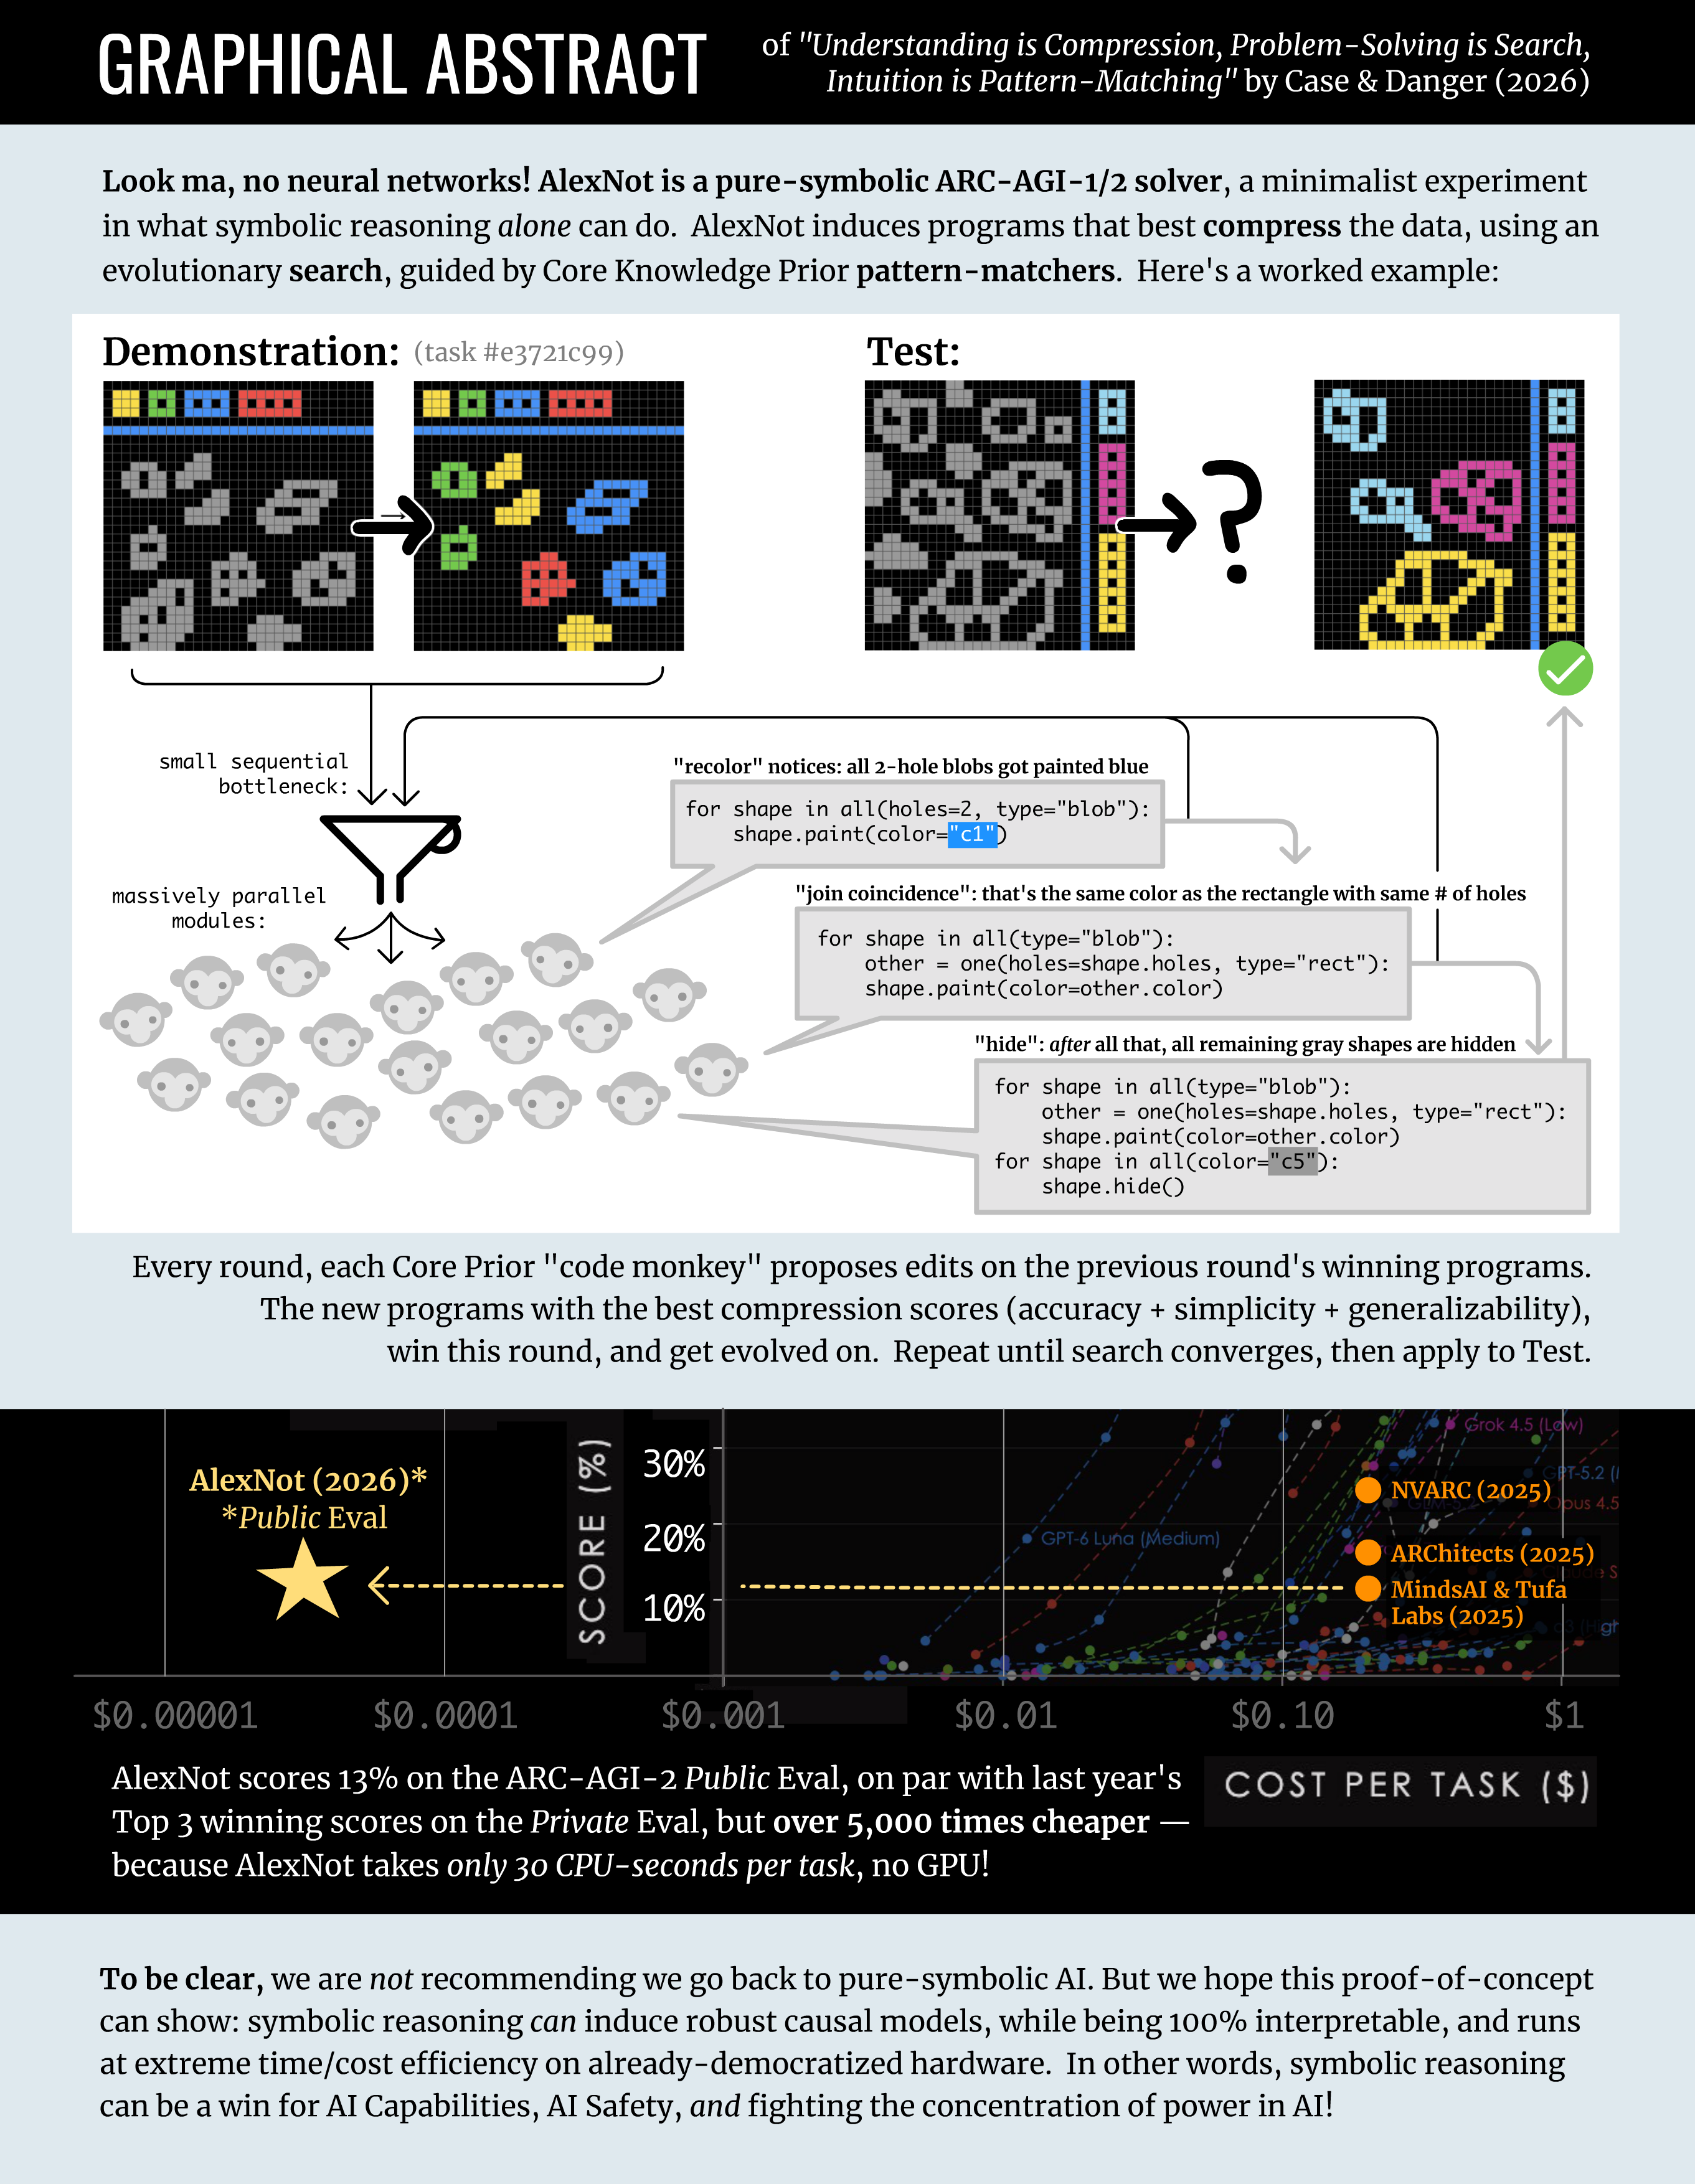
\includegraphics[width=\paperwidth, height=\paperheight, keepaspectratio]{figures/full/COVER.png}
\restoregeometry
\clearpage
\pagenumbering{arabic}

%%%%%%%%%%%%%%%%%%%%%%%%%%%%%%%%%%%%%%%%%%%%%%%
% ABSTRACT %%%%%%%%%%%%%%%%%%%%%%%%%%%%%%%%%%%%
%%%%%%%%%%%%%%%%%%%%%%%%%%%%%%%%%%%%%%%%%%%%%%%

% Make abstract match body style, except for changed spacing
\renewenvironment{abstract}
  {
  \section*{Abstract}              % ``Abstract'' heading
  \begin{spacing}{1}               % line spacing (set to 1x, so below pt is exact)
  \fontsize{11}{16}\selectfont     % {font size pt}{baseline skip pt}
  \setlength{\parskip}{0.7em}      % space between paragraphs
  \setlength{\parindent}{1.5em}    % indent on first line of each paragraph
  }
  {\end{spacing}}

% Nice title & Authors
\begin{center}
\setlength{\parskip}{0pt}
{\LARGE\bfseries\begin{spacing}{1.2}Understanding is Compression, Problem-Solving is Search, Intuition is Pattern-Matching\end{spacing}}
\vskip 1.4em
{\large Nicky Case\textsuperscript{1} \& Nora Danger\textsuperscript{2}\par}
\end{center}

\vspace{-3em}
\begin{abstract}

To discover what deep learning is missing, let's see how far we can go with deep learning \textit{missing.}

We present \textsc{AlexNot}: a minimalist experiment in \textit{pure-symbolic} AI — no neural nets — to tackle ARC-AGI, a test of fluid reasoning. AlexNot is a discrete program inductor, inspired by Global Workspace Theory and 3 universal principles from Cognitive Science: \textbf{understanding is compression, problem-solving is search, intuition is pattern-matching.} It finds programs that best \textit{compress} a dataset, using an evolutionary \textit{search}, guided by ``core knowledge prior'' \textit{pattern-matchers}. The reasoning is 100\% human-readable, the architecture is highly modular \& parallelizable, and it finds not just \textit{one} best answer, but a whole approximate Bayesian distribution of answers.

Contrary to widespread expectation, we show that symbolic reasoning \textit{alone} can exhibit non-trivial fluid intelligence! AlexNot scores \textbf{13.33\%} on the ARC-AGI-2 \textit{Public} Eval — on par with the Top 3 \textit{Private} Eval scores from 2025 — but \textit{over 5,000 times} cheaper: \textbf{30 CPU-seconds, or \$0.000035, per task}. On Kaggle contest hardware, AlexNot blasts through all 240 Semi-Private/Private Eval tasks in \textit{under 5 minutes}, giving us plenty of time to ensemble it with last year's \#1 pure-neural solution (NVARC). Our ensemble gets \textbf{31.53\%} on the Kaggle leaderboard, which also shows how neural + symbolic is better than either alone. 

Next, to show AlexNot's generality, we present \textsc{AlexNot-ODE}, which rediscovers \textit{real-world} differential equations — in physics, life sciences, and business — from sparse, noisy time-series data. Finally, we present design sketches for extending AlexNot to ARC-AGI-3 (agentic intelligence) \& ARC-AGI-4 (open-ended innovation), as well as ``business-incentive-gradient-compatible'' ways to make LLMs \textit{convert themselves} to Neuro-Symbolic hybrids.

To be clear, we do \textit{not} think our field should return to pure-symbolic AI. This project is just a proof-of-concept to show: symbolic reasoning \textit{can} help AI induce robust causal world models, while being 100\% interpretable and verifiable, all at extreme time/cost/data-efficiency on already-democratized hardware. In other words: more-symbolic AI could be a win for AI abundance, AI security, \textit{and} fighting the concentration of power in AI.

\vspace{1.5em}
\noindent\rule{\linewidth}{0.5pt}
% Info (left) & cite-me box (right), side by side
\noindent
\begin{minipage}[t]{0.53\linewidth}
\small\setlength{\parskip}{0.3em}
\noindent\textsuperscript{1} \texttt{n@ncase.me} \quad \textsuperscript{2} \texttt{nora@nora.zip}\par
\noindent\textbf{Open Access:} Code \& paper are available at \url{https://github.com/ncase/alexnot} under CC0. Code includes a local webapp for you to try AlexNot yourself!\par
\noindent\textbf{AI Collaboration:} All main text in this paper is human-generated — even these lovely em dashes — check with Pangram.com if you don't believe us. The Claude family assisted with code and research.
\end{minipage}%
\hfill
\begin{minipage}[t]{0.45\linewidth}
\vspace{0pt}% align top of box with top of text
\begin{tcolorbox}[sharp corners, boxrule=0.4pt,
  colframe=black!40, colback=white, left=4pt, right=4pt, top=2pt, bottom=2pt]
\scriptsize\setstretch{1}
\textbf{Cite as:} \url{https://ncase.me/alexnot-paper}
\begin{verbatim}
@misc{alexnot2026,
  author = {Case, Nicky and Danger, Nora},
  title  = {{Understanding is Compression,
    Problem-Solving is Search, Intuition
    is Pattern-Matching}},
  year   = {2026},
  url    = {https://ncase.me/alexnot-paper}
}
\end{verbatim}
\end{tcolorbox}
\end{minipage}
\end{abstract}
\clearpage

%%%%%%%%%%%%%%%%%%%%%%%%%%%%%%%%%%%%%%%%%%%%%%%
% TABLE OF CONTENTS %%%%%%%%%%%%%%%%%%%%%%%%%%%
%%%%%%%%%%%%%%%%%%%%%%%%%%%%%%%%%%%%%%%%%%%%%%%

\begin{spacing}{1.0}
\fontsize{11}{15}\selectfont
\begin{multicols}{2}
\raggedright
\tableofcontents
\end{multicols}
\normalsize
\end{spacing}

\clearpage

%%%%%%%%%%%%%%%%%%%%%%%%%%%%%%%%%%%%%%%%%%%%%%%
% MAIN TEXT %%%%%%%%%%%%%%%%%%%%%%%%%%%%%%%%%%%
%%%%%%%%%%%%%%%%%%%%%%%%%%%%%%%%%%%%%%%%%%%%%%%

%%%%%%%%%%%%%%%%%%%%%%%%%%%%%%%%%%%%%%%%%%%%%%%%%%%%%%%%%%%%%%%%%%%%%%%%%%%%%%%%%%%%%%
%%%%%%%%%%%%%%%%%%%%%%%%%%%%%%%%%%%%%%%%%%%%%%%%%%%%%%%%%%%%%%%%%%%%%%%%%%%%%%%%%%%%%%
% INTRODUCTION 
%%%%%%%%%%%%%%%%%%%%%%%%%%%%%%%%%%%%%%%%%%%%%%%%%%%%%%%%%%%%%%%%%%%%%%%%%%%%%%%%%%%%%%
%%%%%%%%%%%%%%%%%%%%%%%%%%%%%%%%%%%%%%%%%%%%%%%%%%%%%%%%%%%%%%%%%%%%%%%%%%%%%%%%%%%%%%

\twocolumn

\begin{figure*}[b]
    \centering
    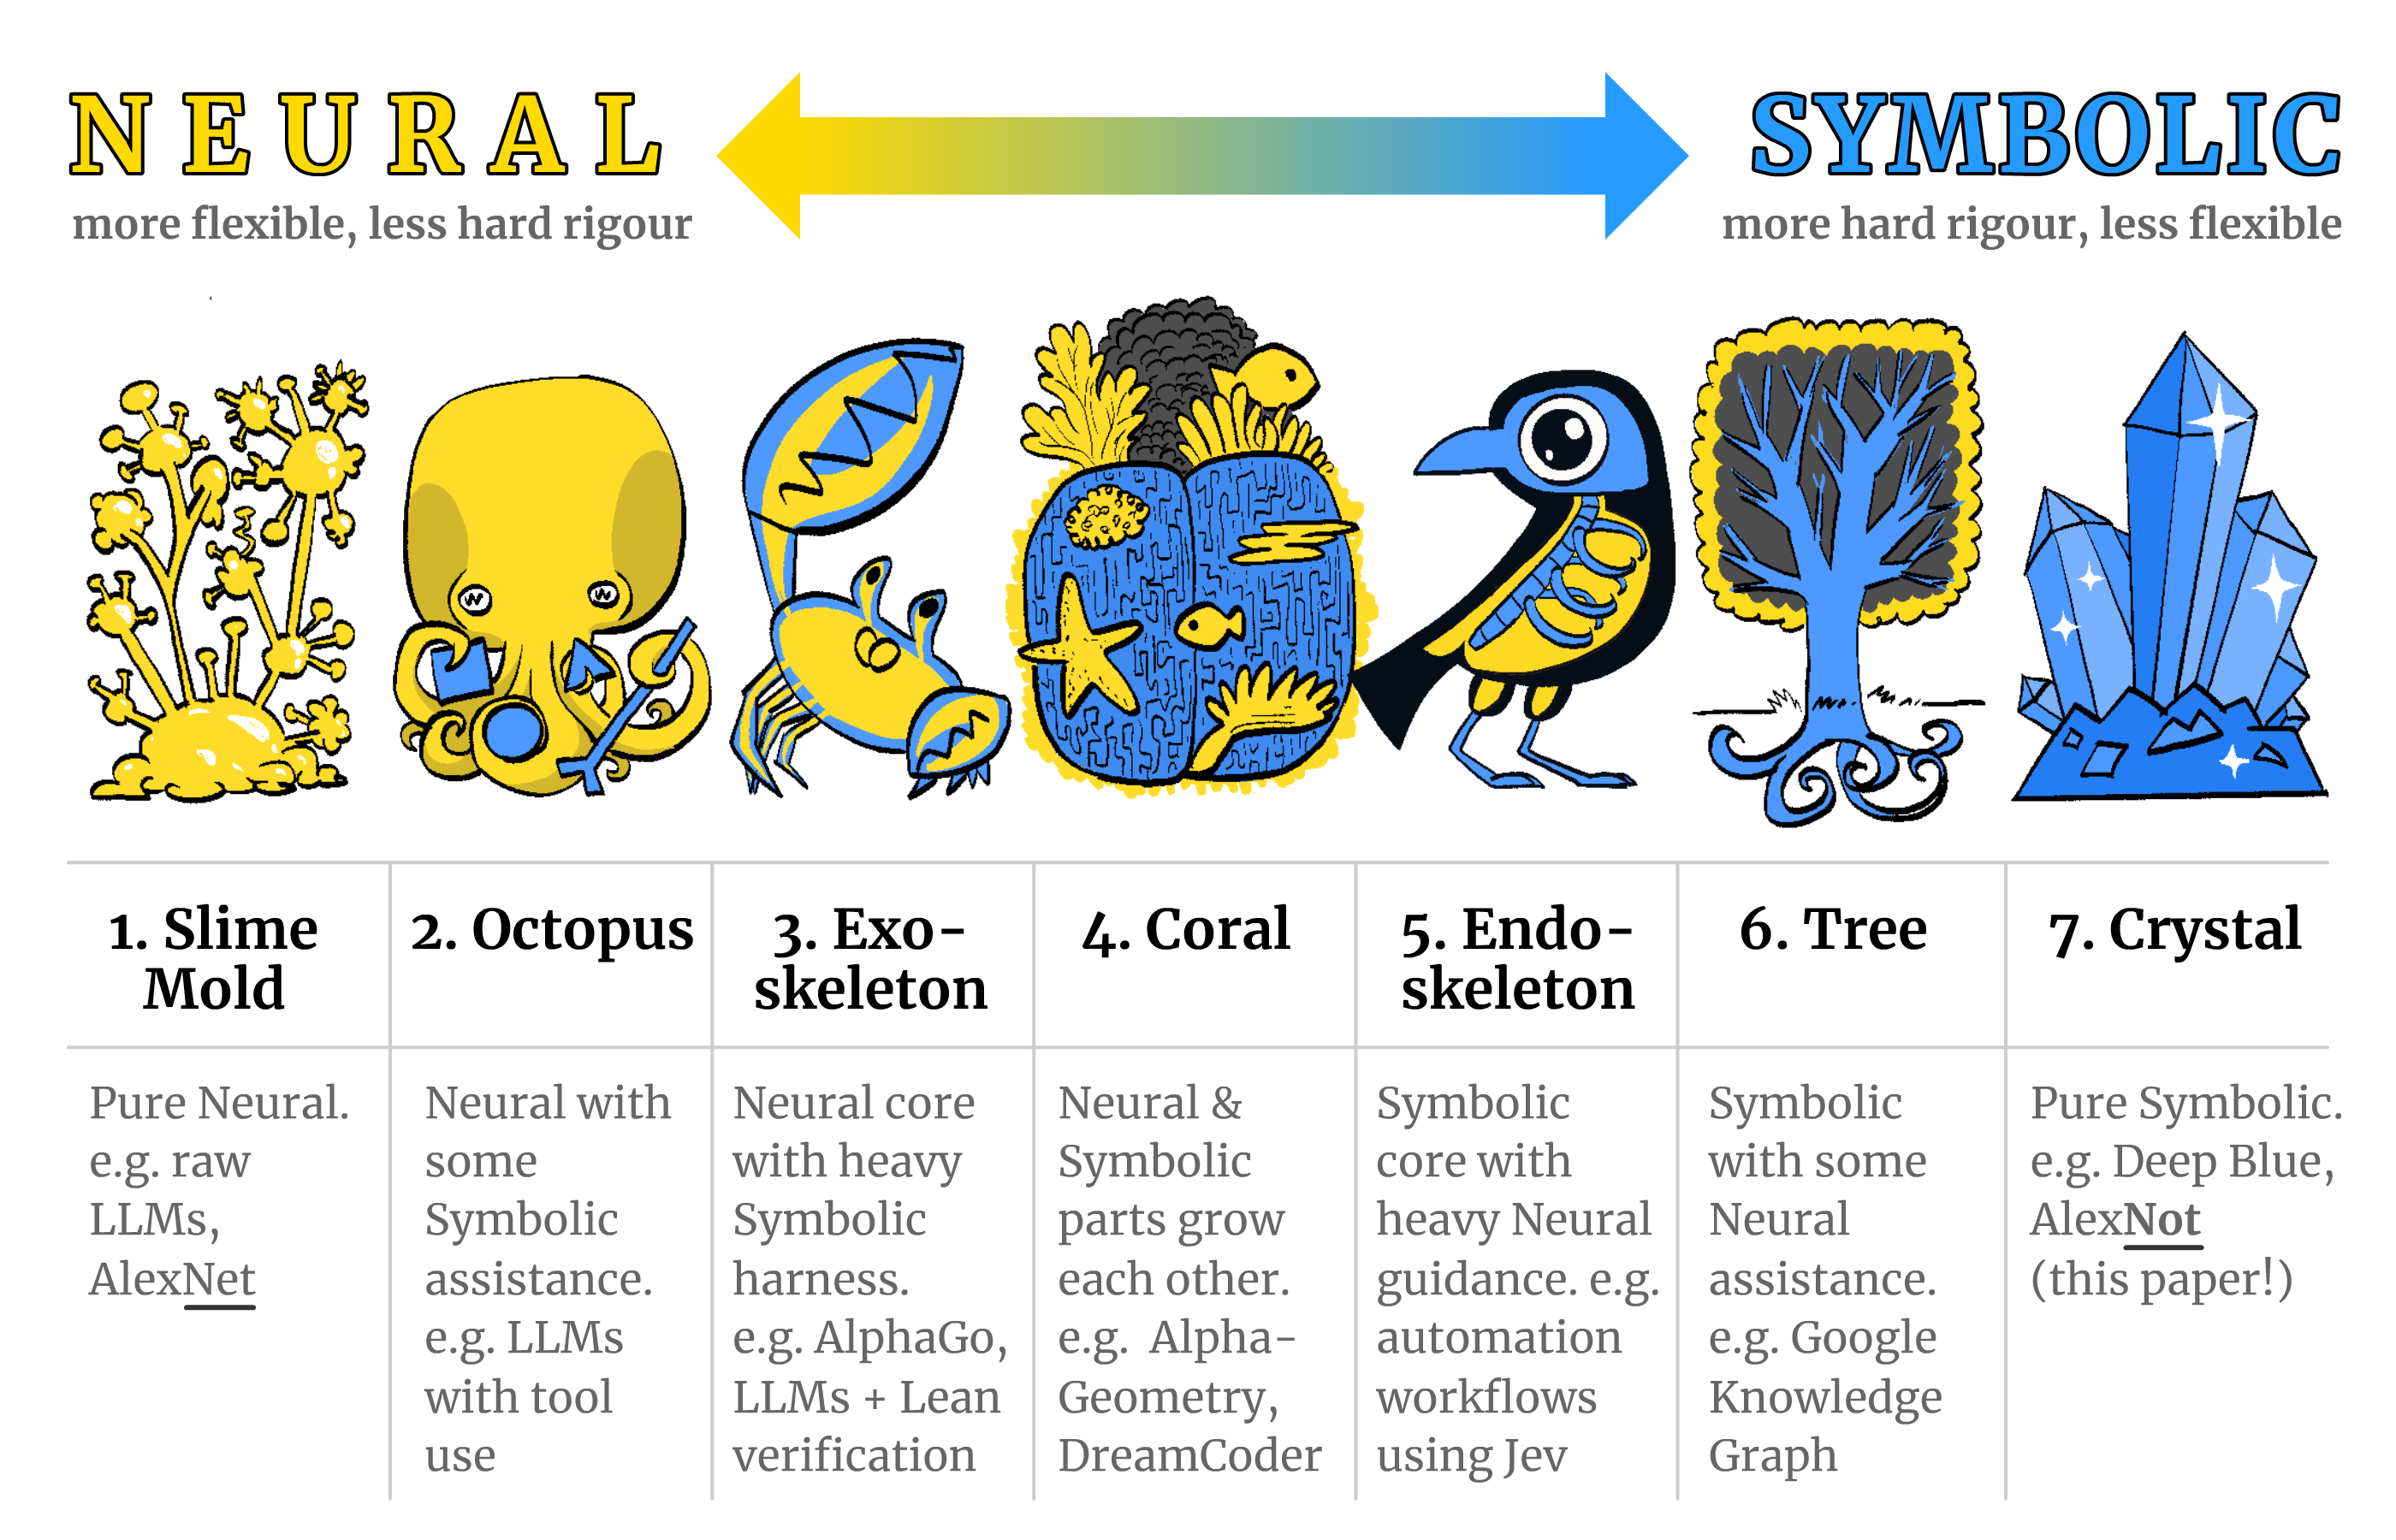
\includegraphics[width=\linewidth]{figures/across/neurosymbolic.png}
    \caption{The Neuro-Symbolic Spectrum as Seven Lifeforms, where neural = soft parts, symbolic = hard parts. And yes I know crystals aren't alive, it's a metaphor not an isomorphism.}
    \label{fig:seven_lifeforms}
\end{figure*}

\section{Introduction}

\subsection{What's Symbolic AI, Neural AI, Neuro-Symbolic AI, ARC-AGI?}

Artificial Intelligence is a spectrum.

On one end, there's \textbf{Symbolic AI}: all facts, skills, and heuristics are explicitly written down as code. On the other end, there's \textbf{Neural AI}\footnote{Also historically called `Connectionist AI'.}: little to no explicit built-in knowledge, just let the universal approximator \citep{universal_approximation} approximate a function from millions of data points. These two approaches map — very loosely — onto `logic' and `intuition', and have the pros/cons you'd expect of pure logic/intuition: Symbolic AI is rigorous but lacks flexibility, Neural AI is flexible but lacks rigour.

But humans have logic \textit{and} intuition.\textsuperscript{[citation needed]} For this reason, many researchers \citep{algebraic_mind,neuro_sym_fdn,bengio_1_to_2,third_ai_summer,third_ai_wave} have long advocated for a Third Wave in AI: \textbf{Neuro-Symbolic AI}, to get the best of both worlds. This phrase, by intention, is a wide umbrella. So in the playful spirit of \citet{five_worlds}'s Five Worlds, see \autoref{fig:seven_lifeforms} for Seven Lifeforms along the neuro-symbolic spectrum. (For other complementary taxonomies of Neuro-Symbolic AI, see \citet{third_ai_summer, third_ai_wave}.)

There's another important distinction to know, between two kinds of intelligence \citep{cattell}: \textbf{crystallized intelligence}, the summed knowledge \& skills from problems you've solved before, and \textbf{fluid intelligence}, the ability to \textit{efficiently} understand \& solve problems you've never seen before. (`efficient' is crucial: with unlimited resources, even zero-intelligence brute-force could solve any task \citep{chollet_intelligence_efficiency}.)

Historically, both Symbolic and Neural AI do fine on \textit{crystallized} intelligence: with Symbolic AI, we directly hand-craft facts \& skills; with Neural AI, we fit a neural network to everything everyone everywhere has ever posted online. However, both approaches struggle with \textit{fluid} intelligence: Symbolic AI fails outside its narrow domain, while Neural AI generalizes poorly outside its training distribution. But, as proponents of Neuro-Symbolic AI argue, the symbiosis of both approaches might unlock \textit{fluid} intelligence for AI.

Which brings us to the \textbf{ARC-AGI} benchmark series! First introduced in \citet{chollet_intelligence_efficiency}, long before LLMs went mainstream, the \textit{Abstraction and Reasoning Corpus for Artificial General Intelligence} (ARC-AGI) is a test of \textit{fluid} intelligence for AI, similar in spirit to the Bongard Problems \citep{bongard_problems} or Raven's Progressive Matrices in human IQ tests \citep{raven_matrices}. Contrary to popular misconception, the benchmark was \textit{not} designed to detect ``are we there (AGI) yet'', but to detect \textit{the bare minimum} level of fluid general intelligence; the original ARC-AGI is to novel reasoning, as MNIST is to machine vision.

ARC tasks are designed to be easy — even fun! — for humans, but hard for AI. Here's how ARC-AGI-1 (2019) and ARC-AGI-2 (2025), the first two benchmarks in the series, worked.\footnote{The main improvements from ARC-AGI-1 to ARC-AGI-2 were: all puzzles solvable with brute-force were removed, the tasks were calibrated using empirically-tested human performance, and puzzles now usually had 2 or more hidden rules composed together. \citep{arc_agi_2}} You get 2 to 6 before-after pixel grid pairs, demonstrating a hidden rule. Your goal is to figure out the rule — ``rule induction/abduction'', as the cool scientists say\footnote{Annoying terminology note: ``induction'' in computer science, philosophy of logic, and mathematics \textit{all have different meanings}. Induction (CompSci) = Abduction (Philosophy) = figuring out most likely theories given data. Induction (Philosophy) = inferring that if X has always happened before, it'll happen again next time. Induction (Mathematics) is a form of \textit{Deduction} (Philosophy) = if you prove Case 0 and prove If Case N then Case N+1, you prove all Case N. In this paper, we'll always mean induce = abduce = best theory from data.} — and apply that rule to the test grids. In a sense, \textbf{ARC-AGI is science in miniature}: observe, theorize, apply, repeat. (See \autoref{fig:arc_1_2})

\begin{figure}
    \centering
    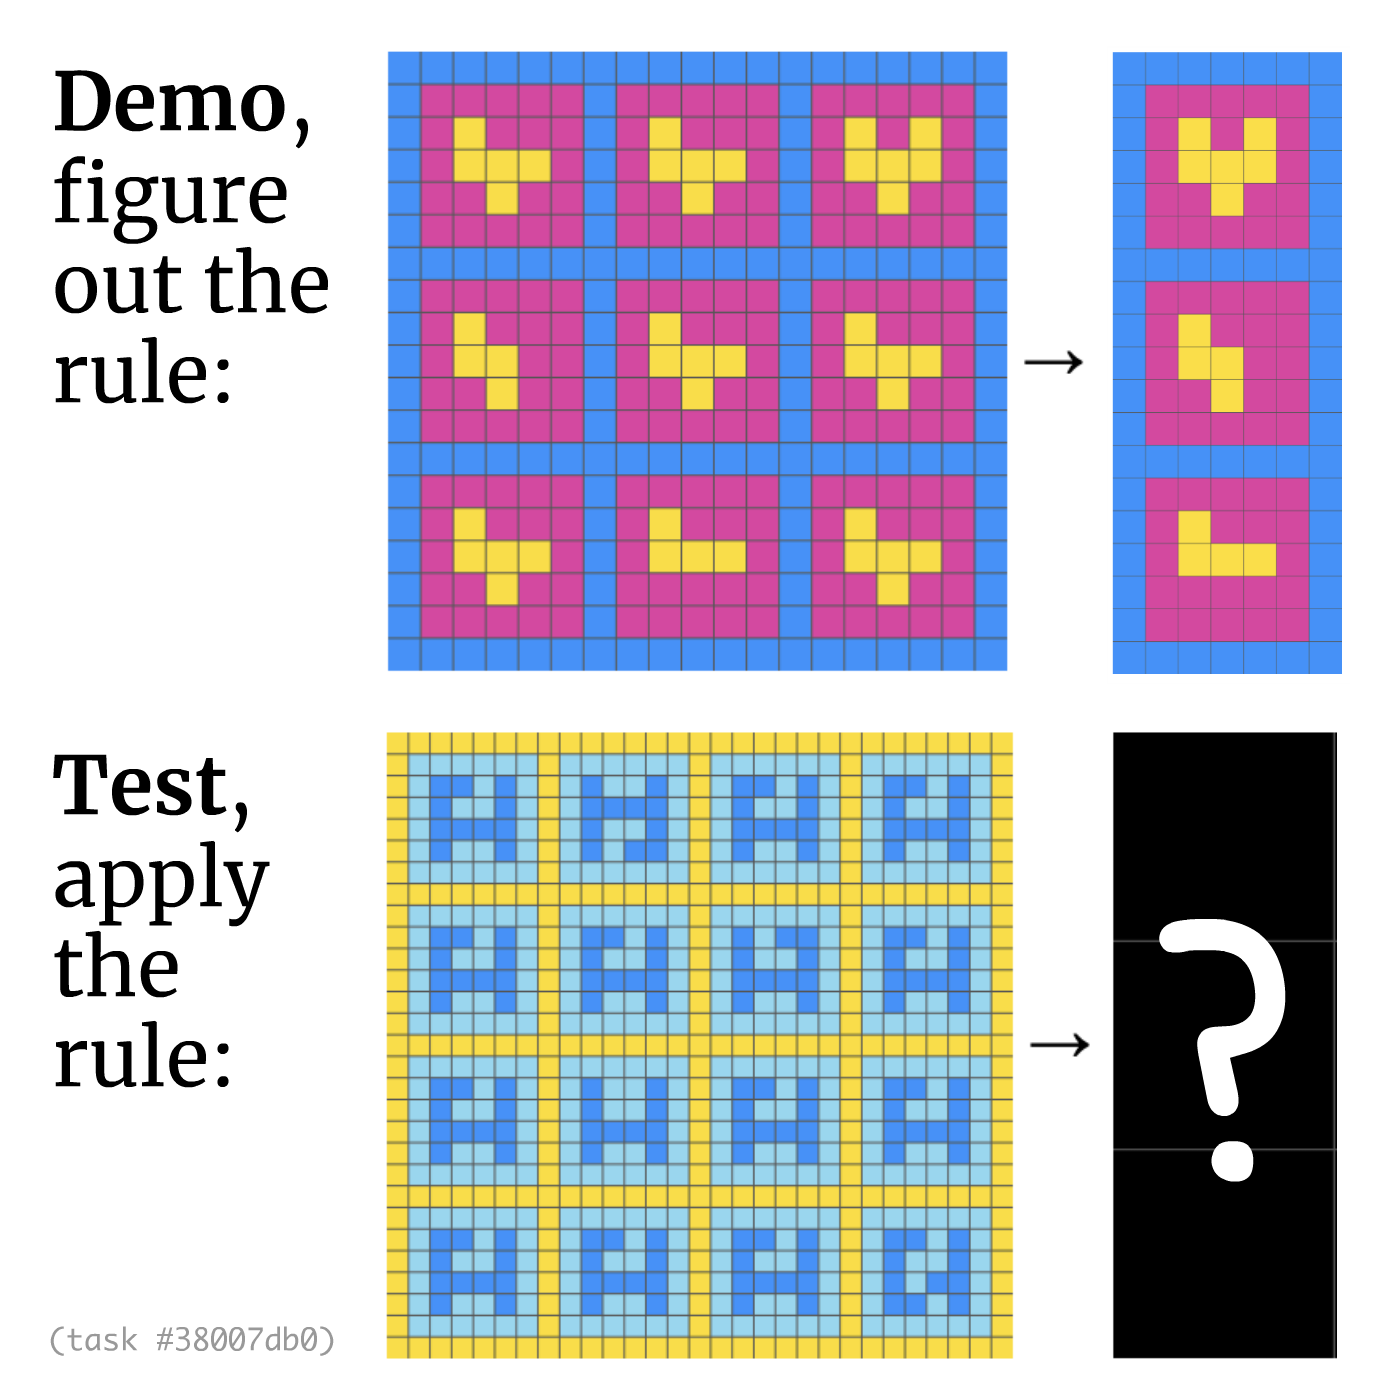
\includegraphics[width=\linewidth]{figures/mini/arc.png}
    \caption{An example of the original ARC-AGI task format}
    \label{fig:arc_1_2}
\end{figure}

Importantly, \textit{no two tasks have the same rule; every rule is unique.} This hits the weak spots of both Symbolic AI (rules can't be hard-coded in advance) and Neural AI (with only 2–6 examples, that's too little data for traditional deep learning). But to make tasks fair, all hidden rules use \textit{only} the ``Core Knowledge Priors'' \citep{core_knowledge_priors}, concepts that are near-universal to all humans: movement, counting, same-different, etc. In practice, most people can solve most tasks, with a median attempt time of 2.3 minutes \citep{arc_agi_2}.

ARC-AGI-3 \citep{arc_agi_3}, the newest benchmark, follows the same design principles, but using interactive mini-games! Each game has a unique set of hidden rules, that you need to figure out on your own, and use to win. This tests fluid intelligence \textit{combined} with agentic intelligence. ARC-AGI-4, at the time of this writing, has no official release material, but it's been teased it will specifically target ``open-ended innovation'' \citep{arc_agi_4_announcement}. (Contrary to criticism, this is not ``moving the goalposts'', this is \textit{upgrading} our goalposts. ARC-AGI-1 to -2 to -3 $\approx$ MNIST to CIFAR-100 to ImageNet.)

\textbf{So how have Symbolic and Neural AI done on ARC-AGI?} Interestingly, it's recapitulated the history of Symbolic/Neural AI in the field at large \citep{third_ai_wave}: overwhelmingly Symbolic, then overwhelmingly Neural, and now mostly Hybrids. In the first ARC-AGI contest, the \#1 solution \citep{icecuber} was pure-symbolic, but used brute-force search. In the second ARC-AGI contest, the \#1 solution \citep{architects_2024} was now pure-neural, and didn't even do program induction/abduction, it just directly predicted the outputs (`transduction'). In the third ARC-AGI contest — now using the updated ARC-AGI-2 dataset, which was harder, and removed all brute-force-able tasks — the \#1 solution \citep{nvarc_2025} used the same pure-neural direct-prediction approach as the previous year, but trained on 3.2 million synthetic examples.

But finally, for ARC-AGI-3, we saw the rise of (slightly more) symbolic solutions: frontier LLMs \textit{with programmatic harnesses} could get near-perfect (non-official) scores on the early preview games \citep{hill_climbing_arc_3} and full Public Demo games. \citep{prolong_arc_3,retrodict_arc_3} In September 2026, GPT-6 Astra with \textit{Provider Adapter harness}\footnote{The ``Provider Adapter'' harness lets the model use custom context-management tools, which the ARC Prize Foundation can't access.} got a score of 99.9\% on the Semi-Private Eval (62.7\% with Standard harness), by building compressed algebraic notations for the games.\footnote{Alas, GPT-6 Astra is mixed news for symbolic reasoning: while it used algebraic notation for \textit{these} ARC games, in general, Astra `thinks' less in transparent chain-of-thought, more in `opaque recurrence', which AI Security experts call unmonitorable `neuralese'. \citep{astra_neuralese}} \citep{astra_arc_3} Call it hopium, but we believe all this — alongside the rise of Lean verification harnesses, and Jev-like classifiers embedded inside normal code — is part of a larger trend of the AI industry, shifting rightwards on the Neuro-Symbolic Spectrum (see \autoref{fig:seven_lifeforms}).

But we think this trend could go even further! To investigate our suspicion, we went all the way to Level 7: could \textit{pure-symbolic AI} — without neural networks, or brute-forcing it like the first year's ARC winner — demonstrate non-trivial \textit{fluid} intelligence?

\subsection{Okay so what did you actually make}\label{sec:what_we_made}

\begin{figure*}[t]
    \centering
    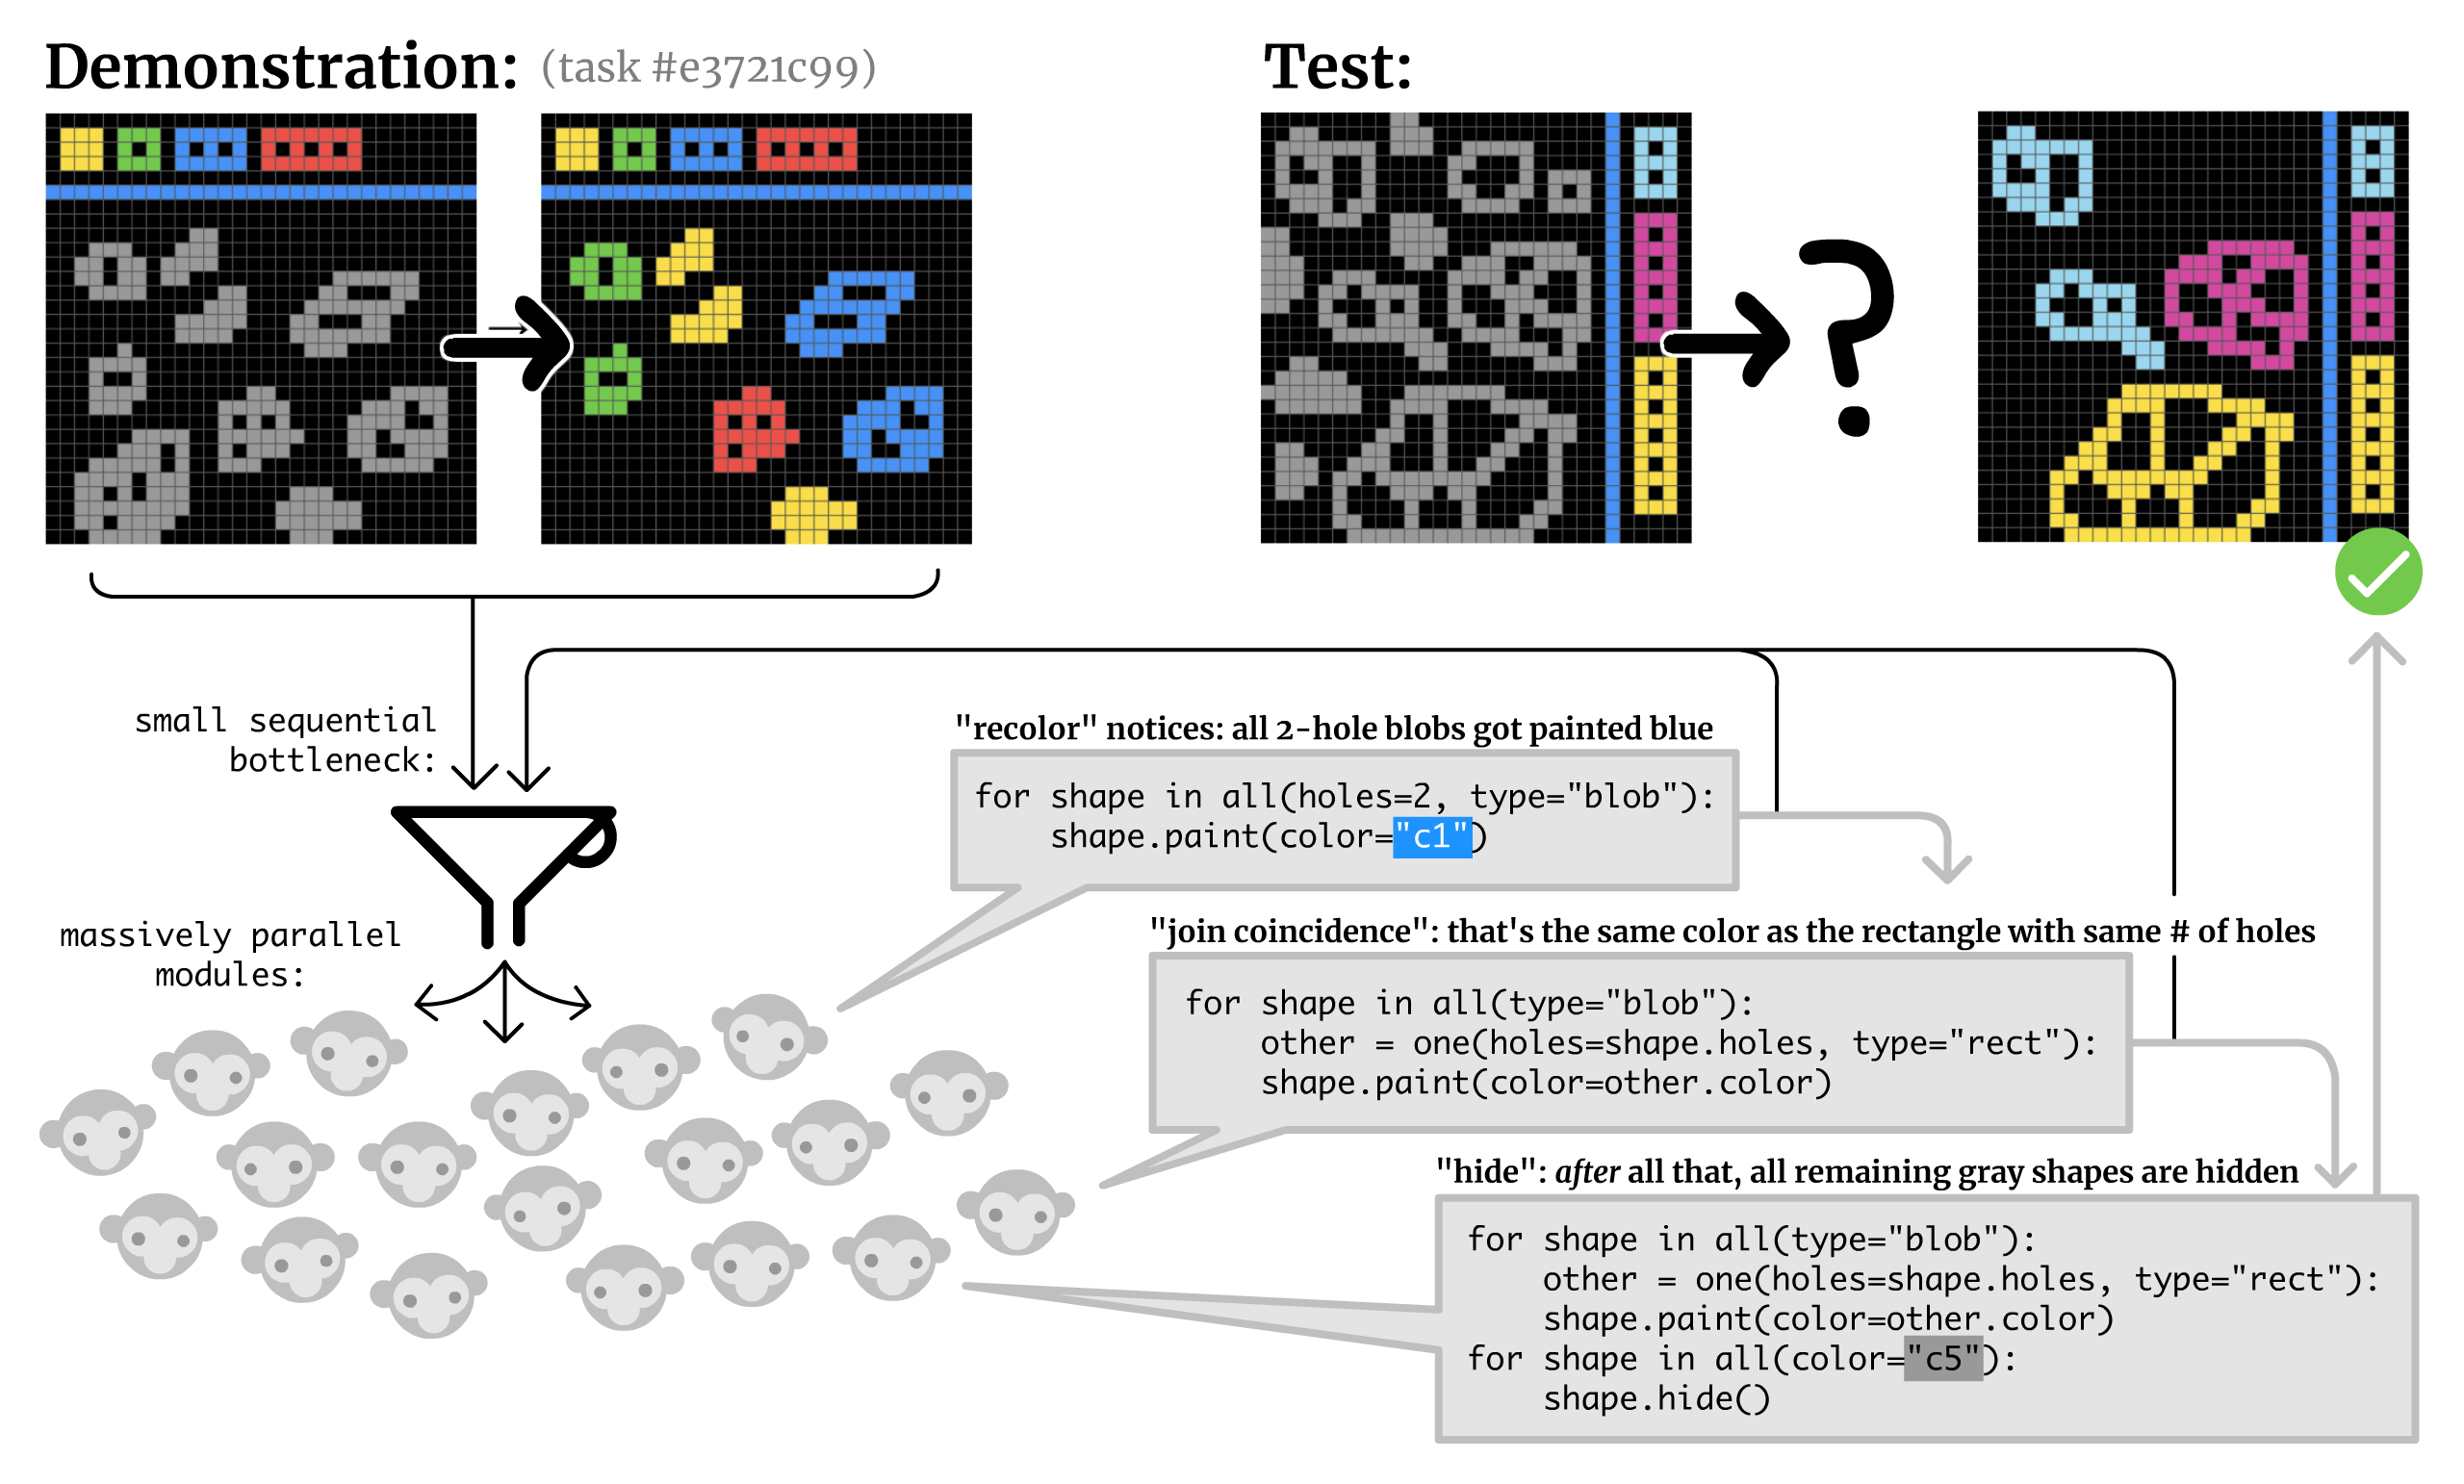
\includegraphics[width=\linewidth]{figures/across/core_loop.png}
    \caption{A worked example of the core AlexNot loop (\textit{simplified schematic}), solving an ARC-AGI-2 Public Eval puzzle. Note how \textit{every} reasoning step produces self-explaining, human-readable programs!}
    \label{fig:alexnot_simplified}
\end{figure*}

\textsc{AlexNot} was directly inspired by 3 universal principles from Cognitive Science: \textbf{understanding is compression, problem-solving is search, intuition is pattern-matching.} Concretely, our solver:

\begin{itemize}
    \item Finds Python programs — written in a domain specific language (DSL) using \textit{only} Core Knowledge concepts (e.g. shape.move(), shape.fall(), etc) — which best \textbf{compress} the data, where compression = simplicity + accuracy in reconstructing the data. If simplicity = prior\footnote{We also added some priors \textit{beyond} code simplicity. Briefly: laziness, familiarity, fewer parameters. We'll explain these more later, but for the sake of simplicity, for now let's just say `simplicity'.}, and accuracy = likelihood, this is analogous to Bayesian inference.
    \item  Our solver finds these programs through a \textbf{search} inspired by Global Workspace Theory \citep{baars_gwt}. Concretely, it's an execution-guided \citep{execution_guided} island-model \citep{island_model} evolutionary search over discrete programs. Each round, dozens of heuristics propose edits to the best programs so far (parallel, bottom-up), the new best programs are selected and broadcast to all heuristics in the next round (sequential, top-down), repeat \& refine until convergence or time's up. By the end, we get not just \textit{one} best program, but a whole Bayesian posterior distribution of possible programs, approximated by applying a softmax to their simplicity + accuracy scores. We even mimic a Dirichlet process \citep{dirichlet_process} to estimate out-of-model uncertainty\footnote{Conceptually similar to ``Knightian Uncertainty'', but by definition Knightian Uncertainty is supposed to be unquantifiable.}, so it can ``know when it doesn't know''.
    \item The aforementioned \textbf{pattern-matching} heuristics implement the Core Knowledge concepts (e.g. color this, rotate that, etc), plus a few extras like causality, compression, and `try random edits'.
\end{itemize}

See \autoref{fig:alexnot_simplified} for a worked example! Note: we skipped some details; everything will be completely explained later, but the above is the core heart of the solver.

P.S: Our code at \url{https://github.com/ncase/alexnot} also comes with a local webapp interface. Since it's CPU-only and fast, you can watch it batch-attempt whole datasets in minutes, \textit{with} approximated Bayesian posterior over programs \& answers.

\textbf{Scores:} How AlexNot performs on ARC and ARC-like benchmarks, in order of rising difficulty: (with $\pm$3\% variation, due to the random nature of evolutionary search.)

\begin{itemize}
    \item \textbf{40.40\%} on Concept-ARC \citep{concept_arc}, an ARC variant emphasizing the Core Knowledge Priors
    \item \textbf{32.20\%} on Mini-ARC \citep{mini_arc}, an ARC variant that's all 5$\times$5 grids
    \item \textbf{17.63\%} on ARC-AGI-1 Public Eval
    \item \textbf{13.33\%} on ARC-AGI-2 \textit{Public} Eval
\end{itemize}

To the best of our knowledge, \textbf{AlexNot is the first pure-symbolic solver to get a non-trivial, double-digit score on ARC-AGI-2} (which was re-designed from ARC-AGI-1 to remove all brute-force-able puzzles).

Moreover, because AlexNot can blast through all 240 Semi-Private/Private Eval ARC-AGI-2 tasks \textit{in under 5 minutes} on Kaggle contest hardware\footnote{The 4$\times$L4 hardware we were given has 46 CPUs. 240 tasks $\times$ 0.5 CPU-minutes/task $\div$ 46 CPUs $\approx$ 2.61 minutes. Rounding up to 5 minutes, because Kaggle CPUs were up to 1.5$\times$ as slow as our local testing environment.}, we could easily ensemble it with last year's pure-neural \#1 solution, NVARC \citep{nvarc_2025}. Together, the ensemble gets \textbf{31.53\%} on the Kaggle leaderboard.

Of note: while AlexNot has worse \textit{absolute} performance relative to neural approaches, it seems to scale \textit{relatively} better. Going from ARC-AGI-1 to -2, where the puzzles require more combined \& composed Core Priors, AlexNot dropped from 17.6\% to 13.3\% (Public Eval), but Claude Opus 4 Thinking 16K dropped from 35.7\% to 8.6\% (Semi-Private Eval), and Tiny Recursion Model dropped from 40.0\% to 6.3\% (Semi-Private Eval). \citep{arc_leaderboard} (\autoref{fig:log_odds}) These weren't cherry-picked; as we'll detail in \hyperref[sec:main_results]{Main Results}, on a log-odds chart, AlexNot scales better than \textit{almost every major LLM}, going from ARC-AGI-1 to -2. This is exactly what one would predict from the relative strengths/weaknesses of neural/symbolic: Neural excels at \textit{breadth}, but Symbolic excels at \textit{depth}. 

\begin{figure*}[t]
    \centering
    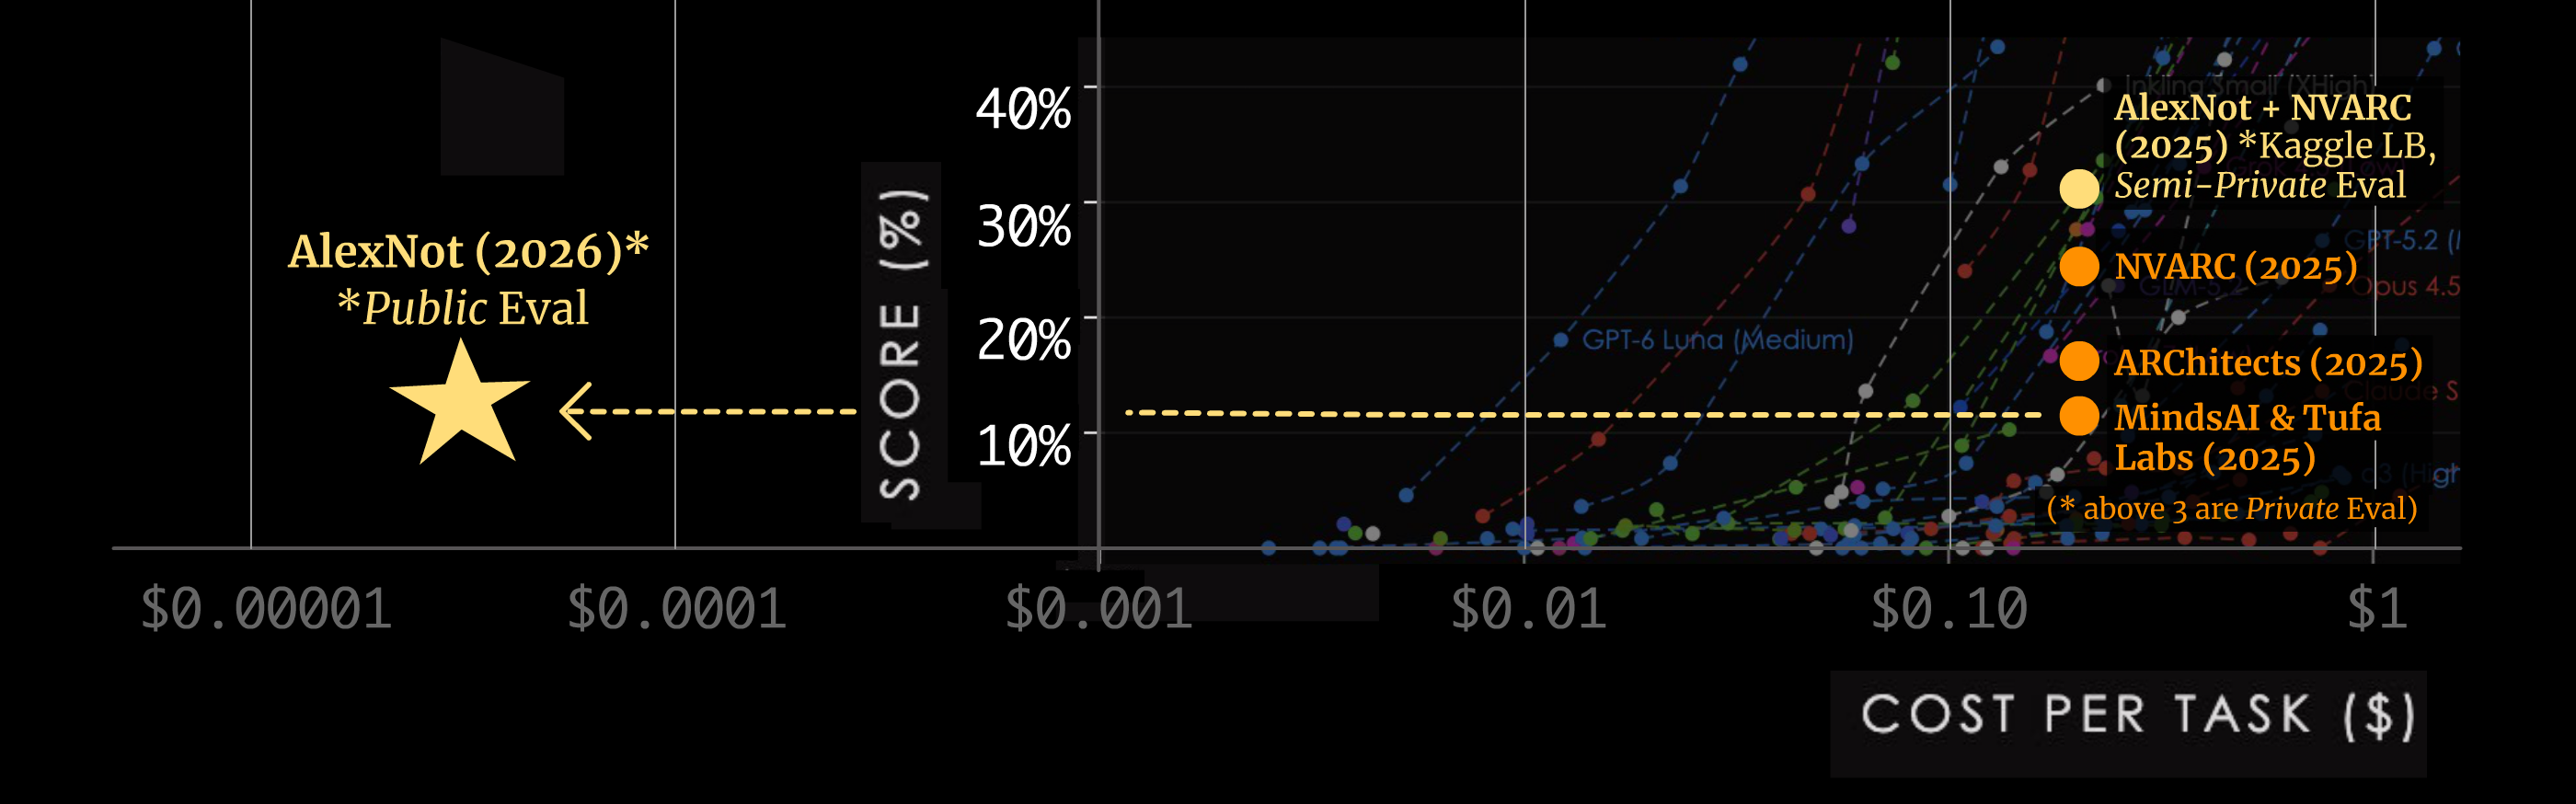
\includegraphics[width=\linewidth]{figures/across/pareto.png}
    \caption{Score vs Cost/task plot for AlexNot (on Public Eval), AlexNot+NVARC (on Kaggle LB/Semi-Private Eval), and 2025's Top 3 Solutions (on Private Eval). \textit{Note:} while the Eval sets are meant to be i.i.d., they're not directly comparable, so take this Figure with a spoon of salt.}
    \label{fig:alexnot_scores_pareto}
\end{figure*}

\textbf{Time/Cost-Efficiency:} The above results definitely don't beat LLMs on raw score, but as \citet{chollet_intelligence_efficiency} argues, intelligence isn't about skill, but skill-acquisition \textit{efficiency}. (You can't data-augment Einstein's papers 'til you get Einstein-on-tap.) And efficiency is where AlexNot shines: on ARC-AGI-2, it spends only \textit{30 CPU-seconds per task, zero GPU}. At the current cloud CPU prices, that's \textbf{\$0.000035 per task}\footnote{AlexNot can run on the cheapest vCPU on AWS, t4g.nano, which at the time of this writing costs \$0.0042 per hour. So at 30 seconds, 30/3600th of an hour, that's \$0.000035 per task. A third of a penny's penny.} — over \textit{5,000 times} more efficient than last year's winning solutions (\$0.20 per task). (\autoref{fig:alexnot_scores_pareto})

\textbf{Universality:} To show that this design isn't limited to ARC-like puzzles — and to show off the benefit of our highly-modular architecture, in contrast to monolithic end-to-end models — in \textit{one} day we vibecoded a variant of AlexNot, that could induce 8 \textit{real-world} differential equations from physics, life sciences, and business, from noisy time-series data. (More details to follow in Results \& Experiments)

Now, if symbolic reasoning is so powerful, why did it fall out of fashion?

To be honest, mostly because of Symbolic AI's expensive disappointments. For example, Cyc. Cyc was a pure-symbolic AI meant to capture all common sense knowledge, and reason effectively \& transparently on it. All this knowledge was coded by hand, and by 2002, Cyc had ``consumed \$60 million and 600 person-years of effort'' \citep{cyc_stanford_2002}. We bring this up pre-emptively, because you'd be right to suspect AlexNot (and any symbolic-first AI) would be haunted by \textbf{\textsc{The Ghost of Cyc}}\footnote{Yes, bold-smallcaps to make it spookier. Happy Belated Halloween, everybody}: the widespread impression that symbolic reasoning was a fragile, expensive dead-end. We hope, for the skeptical reader, this paper can help \textit{exorcise} \textsc{The Ghost of Cyc}, and show you that while it's true that \textit{pure}-symbolic AI (Level 7 on \autoref{fig:seven_lifeforms}) won't scale, symbolic-\textit{heavy} AI with neural guidance (Levels 4, 5, 6) remains a viable path to efficient, trustworthy, open-source AGI. (And as we'll see in the \hyperref[sec:limitations]{Future Research} section, Cyc might have the last laugh after all...)

\subsection{\& So, The Rest Of This Paper}

We are sorry-not-sorry for the sheer amount of \textsc{Theory}\textsuperscript{TM} in this paper. \hyperref[sec:overview]{\textsc{The Galaxybrained Overview}} explains how \textit{pattern-matchers} fit into \textit{search} fit into \textit{compression} fit into \textit{agents} fit into \textit{aligned, self-improving, multi-agent systems}. The next 3 sections go into more detail on each Cognitive Science principle: \hyperref[sec:compression]{\textsc{Understanding is Compression}}, \hyperref[sec:search]{\textsc{Problem-Solving is Search}}, and \hyperref[sec:pattern_matching]{\textsc{Intuition is Pattern-Matching}}. Alongside the theory, we cover relevant prior work, and give complete descriptions of how we implemented these principles in AlexNot. So if you were wondering why such a simple solver is getting a 60+ page paper, it's coz we wanna infodump about \textsc{Theory}\textsuperscript{TM}.

Next, \hyperref[sec:results]{\textsc{Results \& Experiments}} show how AlexNot performed on ARC and ARC-like benchmarks, in comparison with LLMs and other neural solutions. We also do some simple ablation studies to show what mattered for Compression and Search. This is also where we present \textsc{AlexNot-ODE}, a minimal variant of AlexNot that can induce real-world differential equations from sparse, noisy data.

\hyperref[sec:limitations]{\textsc{Summary, Limitations, Future Research}} covers all the flaws of AlexNot, most obviously that it has zero (0) machine-learning component, and thus, was a pain in the posterior distribution to create. But flaws are opportunities, so we sketch out research ideas for extending AlexNot, symbolic reasoning, and the 3 Cognitive Science Principles towards:

\begin{itemize}
    \item How to make progress on ARC-AGI-3 (agentic intelligence) and ARC-AGI-4 (open-ended innovation)
    \item  Business-incentive-gradient-compatible ways for LLMs to \textit{convert themselves} into Neuro-Symbolic hybrids
    \item  A ``Unix Philosophy for AGI'', or ``Peer-to-Peer AGI'': every human gets a one-8-billionth slice of a world wide brain — owned by, validated by, and aligned to \textit{all} of us.
\end{itemize}

Finally, we conclude with \hyperref[sec:conclusion]{\textsc{Conclusion: The Sweet Lesson of Actually Understanding Stuff}}.


\begin{figure*}
    \centering
    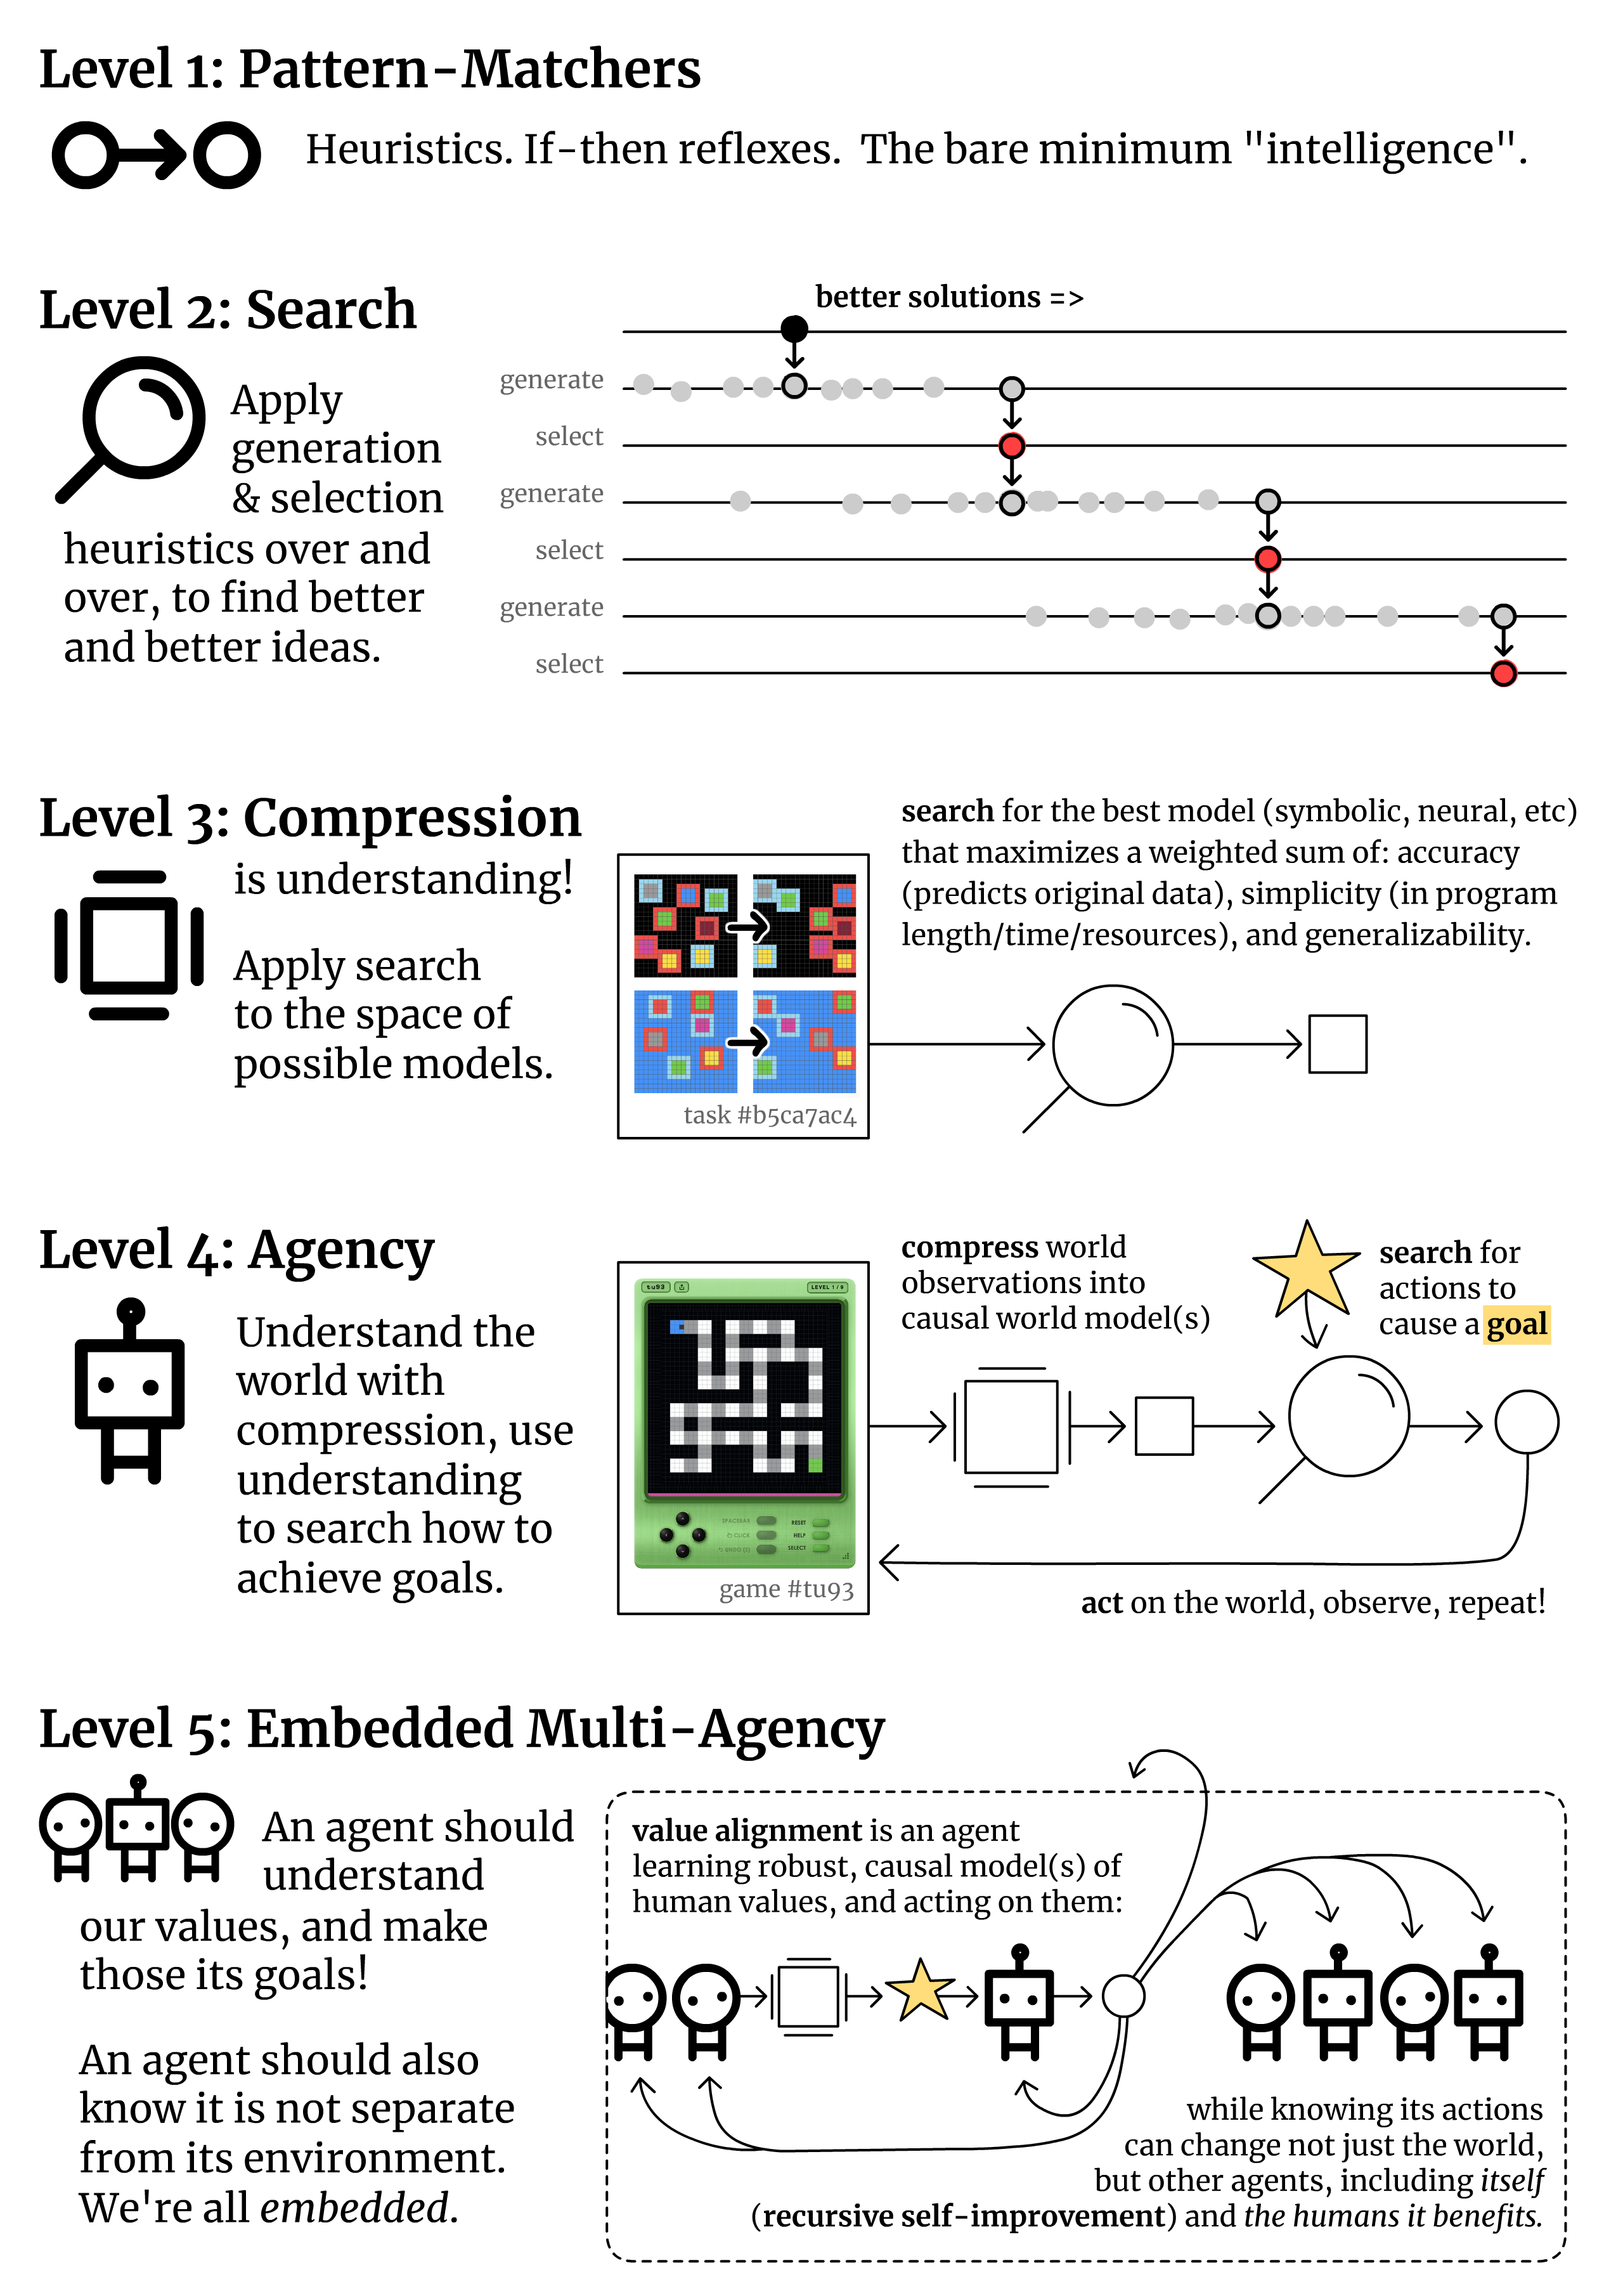
\includegraphics[width=\linewidth,height=0.95\textheight,keepaspectratio]{figures/full/loops.png}
    \caption{Five Loops of Intelligence: Pattern-Matchers $\to$ Search $\to$ Compression $\to$ Agents $\to$ Multi-Agents}
    \label{fig:five_loops}
\end{figure*}


%%%%%%%%%%%%%%%%%%%%%%%%%%%%%%%%%%%%%%%%%%%%%%%%%%%%%%%%%%%%%%%%%%%%%%%%%%%%%%%%%%%%%%
%%%%%%%%%%%%%%%%%%%%%%%%%%%%%%%%%%%%%%%%%%%%%%%%%%%%%%%%%%%%%%%%%%%%%%%%%%%%%%%%%%%%%%
% OVERVIEW 
%%%%%%%%%%%%%%%%%%%%%%%%%%%%%%%%%%%%%%%%%%%%%%%%%%%%%%%%%%%%%%%%%%%%%%%%%%%%%%%%%%%%%%
%%%%%%%%%%%%%%%%%%%%%%%%%%%%%%%%%%%%%%%%%%%%%%%%%%%%%%%%%%%%%%%%%%%%%%%%%%%%%%%%%%%%%%

\section{The Galaxybrained Overview: Loops of Intelligence}\label{sec:overview}

Here's how \textit{pattern-matchers}, fit into \textit{search}, fit into \textit{compression}, fit into \textit{agents}, fit into \textit{multi-agent systems}. (\autoref{fig:five_loops})

In The Beginning, there was the \textbf{Pattern-Matcher} reflex. If this, then that. If see bigger fish, swim away. If temperature too cold, thermostat turns on. Pattern-recognizers can get fairly sophisticated: every ML classifier from the original Alex\textit{\uline{Net}} \citep{alexnet} to ``System 1'' Jev \citep{jev} is basically a pattern-matching heuristic. But from this `atom' of intelligence, we can build molecules:

\textbf{Search.} Most search algorithms — from A* to Evolutionary Algorithms — are fundamentally the same thing: generate candidate solutions, select candidate solutions, repeat to refine. The difference between search algorithms, then, comes down to their generation \& selection heuristics. That is: search is powered by its \textit{pattern-matchers.}

Once we know how to build search in \textit{narrow} domains, we can build something that builds mental models in \textit{general} domains, through:

\textbf{Compression.} Given some data, and an expressive ``language'' to describe models in — Python code, differential equations, causal networks, etc — \textit{search} for the model(s) that most accurately reconstruct that data, while being as simple and generalizable as possible. (Ideally, it should give \textit{a probability distribution} of world models. Remember: ``It ain't what you don't know that gets you into trouble. It's what you know for sure that just ain't so!''\footnote{Often attributed to Mark Twain, but there's no evidence he said it, and the saying's true origins remain unconfirmed. \citep{quote_investigator_aint_so}})

A general Compressor AI would be of great help to science — imagine an AI that could discover Newton's Universal Gravitation from scratch, \textit{using only} pre-Copernican data on the planets' positions — but this AI wouldn't \textit{do} science. It can't design experiments, let alone run them. It can \textit{compress} data to give Newton's laws, but it can't \textit{de-compress} them into useful implications \& inventions. For fully-automated STEM, we need:

\textbf{Agents.} An agent is simply an AI that takes a world model and a goal, then \textit{searches} for the most effective plan to achieve that goal. A \textit{general} agent can create new world models via \textit{compression}, then search over those to achieve goals.\footnote{Note that this is \textit{two different} sub-systems with \textit{different} optimization-targets. The world-modeller is \textit{only} selecting for accuracy+simplicity, while the actor is selecting for some other goal(s). The human brain must also work this way, \textit{separation} of how to learn facts and acts: otherwise, it'd be impossible to learn emotionally-neutral or negative facts, and/or we'd act in the most prediction-error-minimizing way: doing nothing.} (This capability is what ARC-AGI-3 tests.)

Needless to say, a general agent would already be very powerful... but still not enough. The problem is, it can \textit{learn} about the world, but it has to be \textit{given} its goal, and if your formal specification of a goal is even slightly incomplete, by default, the agent will do undesirable things. This is the value alignment problem in AI Safety. \citep{human_compatible} While ``alignment'' is usually talked about in the context of catastrophic loss-of-control AI risks, it's \textit{also} just good business. Any time your coding agent spirals off on a tangent, or does a hacky fragile fix, that's misalignment in miniature. More seriously: why would you rent an AI that \textit{might} hack your own company? (cf. the OpenAI–Hugging Face incident \citep{metr_hf_investigation}.) You wouldn't hire an employee who's not mission-aligned, why would you rent an AI that's not \textit{anything}-aligned? So even if you're skeptical of AI risk, if you don't want code-slop \& science-slop, you need AI that understands what \textit{you} actually value. For that, we need:

\textbf{Embedded Multi-Agency.} The insight: an AI agent can get \& request data from a human (surveys, open-ended conversations, what they say/do/choose, etc), then \textit{compress} that to get (a probability distribution over) robust causal models, of what that human \textit{actually values}. (See: inverse reinforcement learning \citep{inverse_rl}, RLHF \citep{rlhf}, indirect normativity \citep{superintelligence}) Sure, human values are complex, change over time, every measure is a noisy proxy, and the act of measurement or prediction \textit{changes the thing itself} — but the same is true in biological or economic modelling. Modelling human values is hard, but it's not categorically different. (``AI Alignment As Normal ML Problem''?\footnote{Riff off ``AI As Normal Technology'' \citep{ai_normal_technology}})

Furthermore, an AI agent that properly understands how it's \textit{embedded} in the world — there is no real agent/environment distinction — would be able to safely self-modify and self-improve \citep{everitt_self_modification,godel_machine}, and even help us change our values \textit{in a way we'd value}. (See: legitimate value change \citep{value_change_problem}, and causal incentives \citep{causal_foundations_tutorial,agent_incentives_causal})

That is: AI that helps humans be more human(e).

. . .

But wait, you may ask, does this framework prove too much? If creating a provably beneficial AGI with Recursive Self-Improvement (RSI) is just a few compression \& search loops tied together, then — given a starter pack of mere pattern-matching \textit{heuristics} — the algorithm that Creates God is, what, a couple hundred lines of code?

Yes.

Which means the power is \textit{almost entirely in the ``starter pack'' of priors \& pattern-matchers}. RSI is easy. You just get a search algorithm to find a better search algorithm, switch over to that, repeat. This is not a new claim: see Schmidhuber's Gödel Machine \citep{godel_machine} for a concrete example, and \citet{schmidhuber_rsi_since_1987} for a list of concrete RSI algorithms since 1987. The problem is getting a powerful-enough search algorithm in the first place, which means needing powerful-enough generator \& selector heuristics: the ``starter pack''.

(This isn't the same as, but it rhymes with, the oft-misunderstood No Free Lunch Theorem \citep{no_free_lunch}. Loosely paraphrasing, the theorem states: \textit{no optimization algorithm can do better than any other, across the uniform distribution of all possible optimization problems.} On one hand, that's obviously false: science works universally better than random guessing. But the insight is in the flipped view: since no optimization algorithm works better than any other \textit{if we can't assume anything about the problem space}, then the power of any optimization algorithm comes \textit{entirely from its ``starter pack'' of assumptions, the priors.} It's a mystery \textit{why} our Universe seems to have a prior towards simple, composable laws with cause-and-effect — rather than pure uniform-random entropy — but it's a prior assumption we can, and do, fruitfully make.\footnote{This isn't a philosophy paper, but one idea is that it's literal survivor bias, or `anthropics': since the No Free Lunch Theorem implies that useful intelligence/optimizers can \textit{only} exist in universes that aren't uniform-random, that's why we find ourselves here \& now, instead of the Random-Verse or our Universe's heat death 10\textsuperscript{100} years from now.})

So, if \textbf{all the power is in the starter pack}, what should be our starter pack for Compression, Search, and Pattern-Matching?





%%%%%%%%%%%%%%%%%%%%%%%%%%%%%%%%%%%%%%%%%%%%%%%%%%%%%%%%%%%%%%%%%%%%%%%%%%%%%%%%%%%%%%
%%%%%%%%%%%%%%%%%%%%%%%%%%%%%%%%%%%%%%%%%%%%%%%%%%%%%%%%%%%%%%%%%%%%%%%%%%%%%%%%%%%%%%
% UNDERSTANDING IS COMPRESSION 
%%%%%%%%%%%%%%%%%%%%%%%%%%%%%%%%%%%%%%%%%%%%%%%%%%%%%%%%%%%%%%%%%%%%%%%%%%%%%%%%%%%%%%
%%%%%%%%%%%%%%%%%%%%%%%%%%%%%%%%%%%%%%%%%%%%%%%%%%%%%%%%%%%%%%%%%%%%%%%%%%%%%%%%%%%%%%



\begin{figure*}[t]
    \centering
    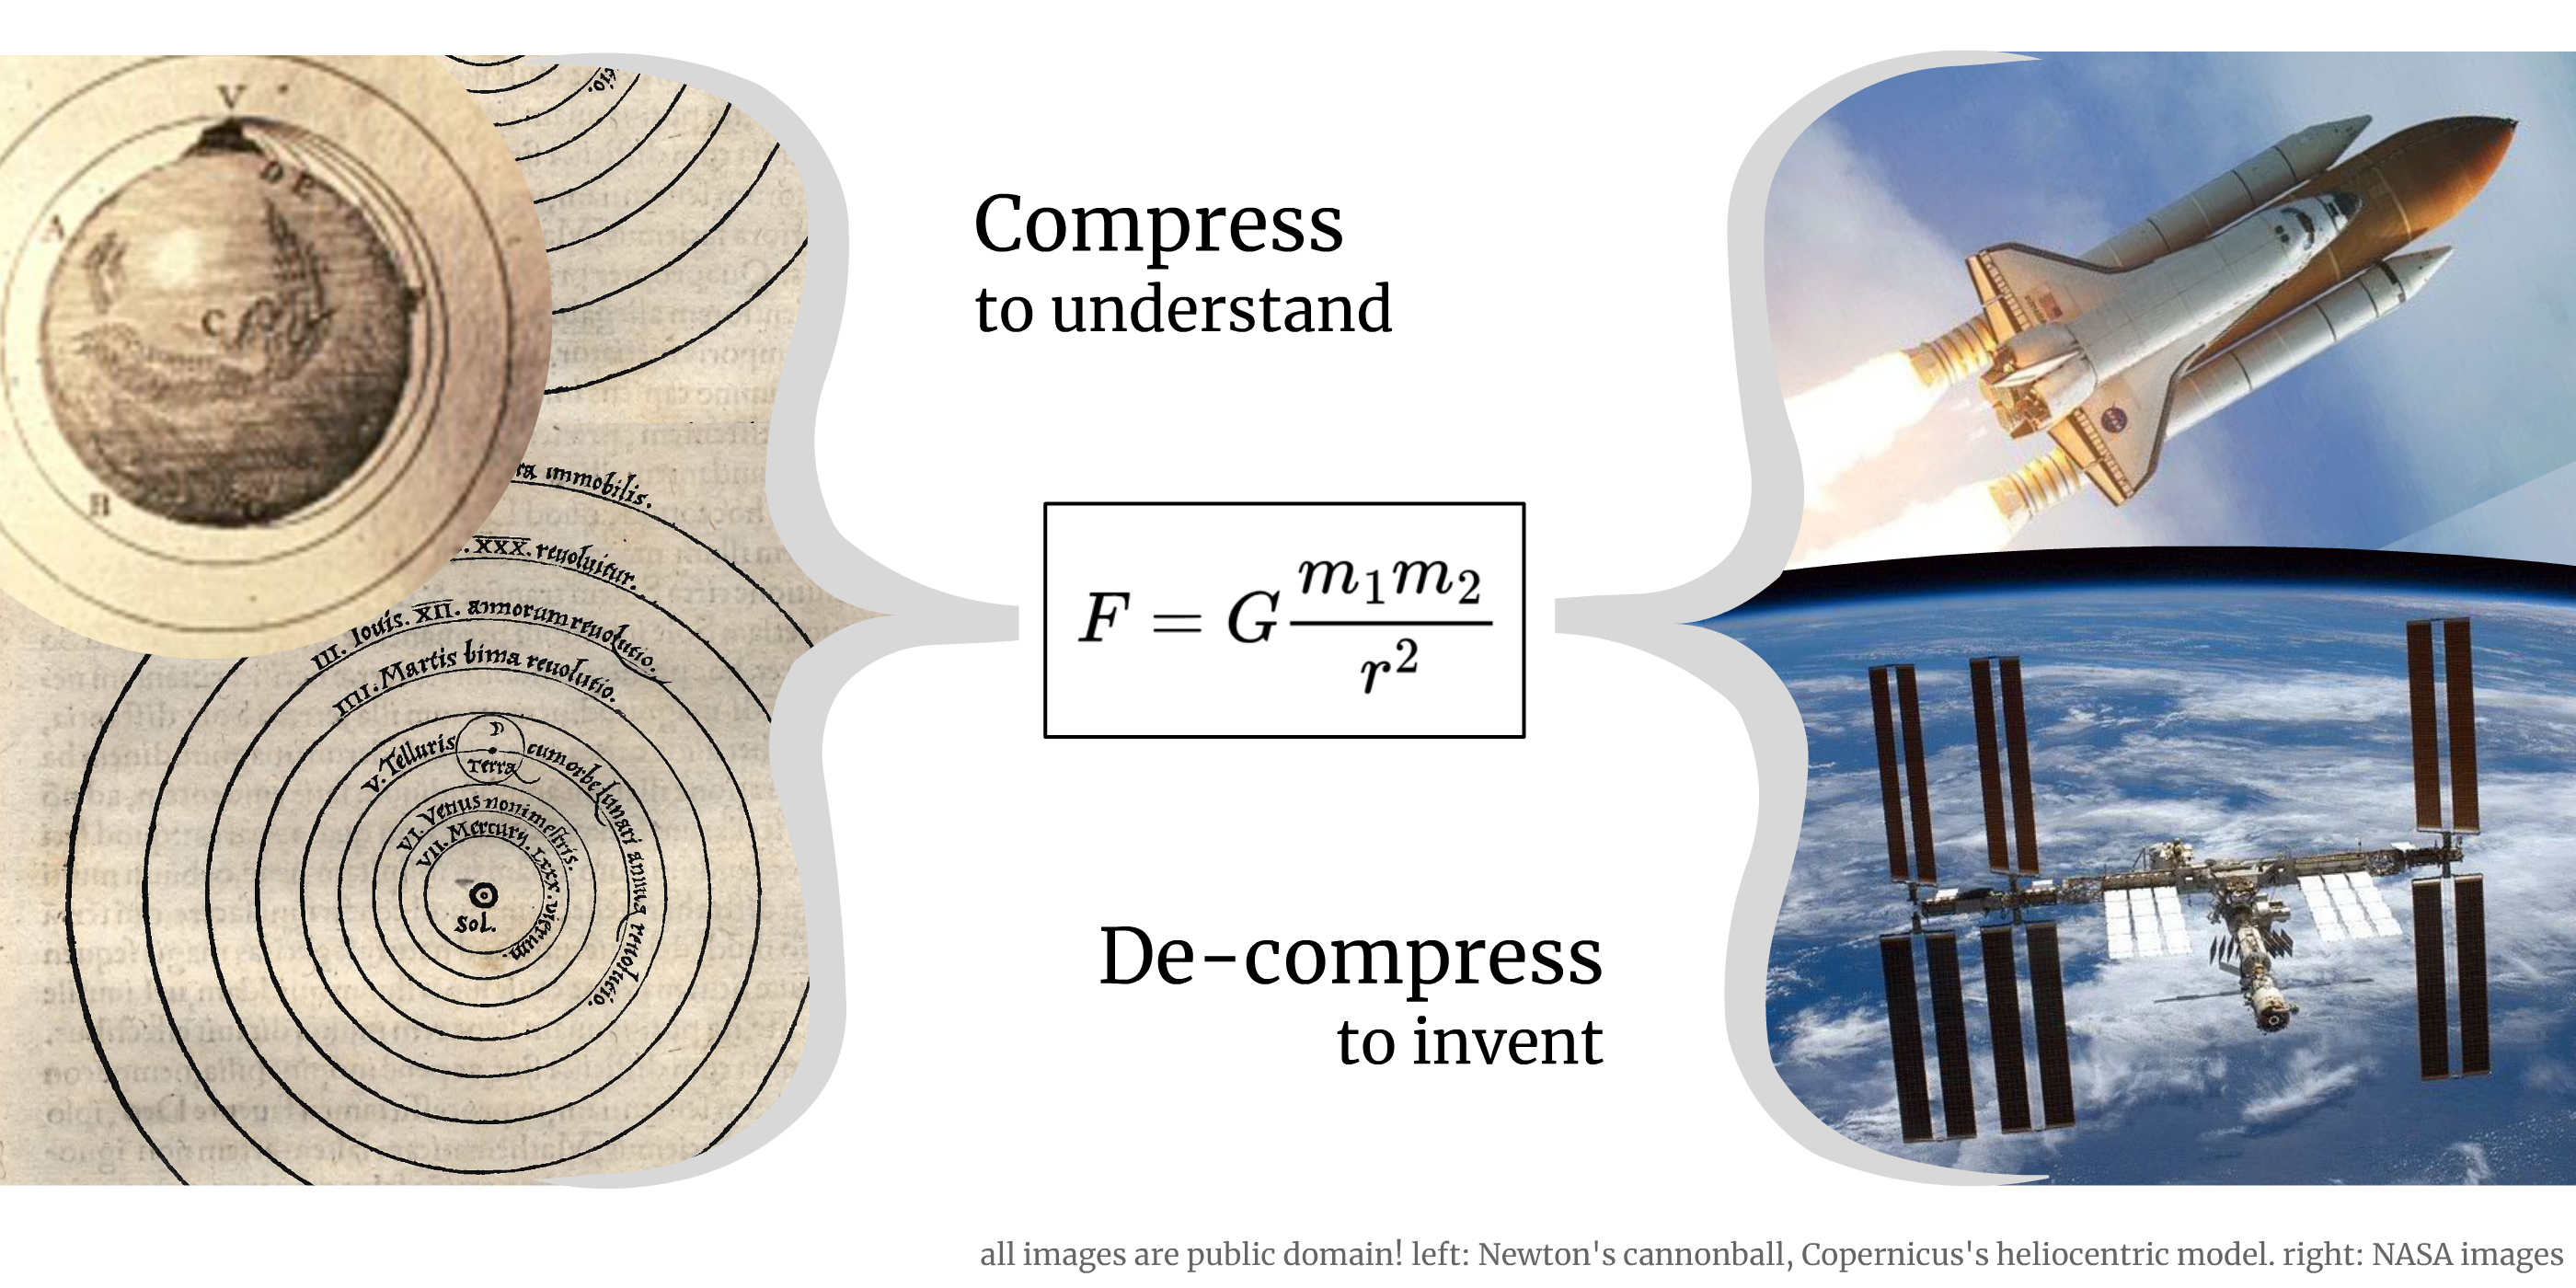
\includegraphics[width=\linewidth]{figures/across/newton.png}
    \caption{Newton compressed the motions of celestial bodies, into a Post-It Note sized formula — which we could then de-compress into making \textit{new} celestial bodies of our own.}
    \label{fig:newton}
\end{figure*}

\section{Understanding Is Compression}\label{sec:compression}

\subsection{The unreasonable effectiveness of compressing data}

\begin{quote}
“Science is, at root, just the search for compression in the world.”

— Cosmologist John D. Barrow \citep[p.~247]{barrow_pi_in_the_sky}
\end{quote}
The `compression' that most people are familiar with, is file compression: take some data, find redundancies (repeated text, repeated video frames), and factor them out to get smaller files, which can be used to reconstruct the original data. \textit{This is like science:} take some data, find regularities (patterns, structure), and abstract them out to get simpler models, which can be used to re-predict the original data — and predict \textit{new} data, and engineer \textit{new} inventions.

Or, since simpler explanations are better: ``simpler explanations are better''.

Humanity keeps rediscovering this idea:

\begin{itemize}
    \item In antiquity: the most famous framing of ``all else equal, simpler theories are better'' is Occam's Razor, but the earliest recording of this maxim goes all the way back to Aristotle \citep{sep_simplicity}.
    \item  In computer science: In the 1900s, ``Understanding is Compression'' finally got a mathematical backbone. See: Shannon 1948 \citep{shannon_entropy}, Kolmogorov Complexity \citep{kolmogorov_complexity}, Minimum Description Length \citep{rissanen_mdl}, Solomonoff Induction \citep{solomonoff_induction}. AIXI \citep{aixi} is a theoretical formalism for AGI combining Occam's Razor with expected utility. AIXI's author even founded The Hutter Prize \citep{hutter_prize}, an ongoing €500,000 contest to compress 1GB of Wikipedia text, created specifically on the premise that compression and intelligence are fundamentally related.
    \item In cognitive science: The free energy principle \citep{free_energy_principle} proposes the brain does Bayesian inference, by minimizing surprise \& complexity — or equivalently, reconstructing the original sense data as simply as possible: compression. Separately, \citet{wolff_intelligence} proposes intelligence \textit{is} compression, and \citet{schmidhuber_driven_by_compression} proposes that the \textit{first derivative} of compression drives curiosity \& aesthetics.
    \item In deep learning: One hypothesis why Stochastic Gradient Descent works so well is because it indirectly implements the MDL (Minimum Description Length) principle: SGD tends towards flat minima, which require less precision to specify, that is, \textit{fewer bits} of information \citep{flat_minima,large_batch_sharp_minima}. Meanwhile, auto-encoders \citep{hinton_autoencoder} are a more direct form of compression: just re-predict the original input using a much smaller embedding.
    \item In ARC-AGI: In \citet{arc_without_pretraining}, the authors find that \textit{simply compressing the target puzzle}, into a 76K parameter model, with no pretraining, lets it solve 20\% of ARC-AGI-1 Public Eval puzzles!
    \item In LLMs: You can use an LLM to \textit{quadruple} the compression ratio for text \citep{compress_with_llm}, and — coming full circle — you can even do the reverse: an everyday file compressor like .gzip can be used \textit{as a language model}. \citep{gzip_llm}
\end{itemize}

\begin{figure*}[t]
    \centering
    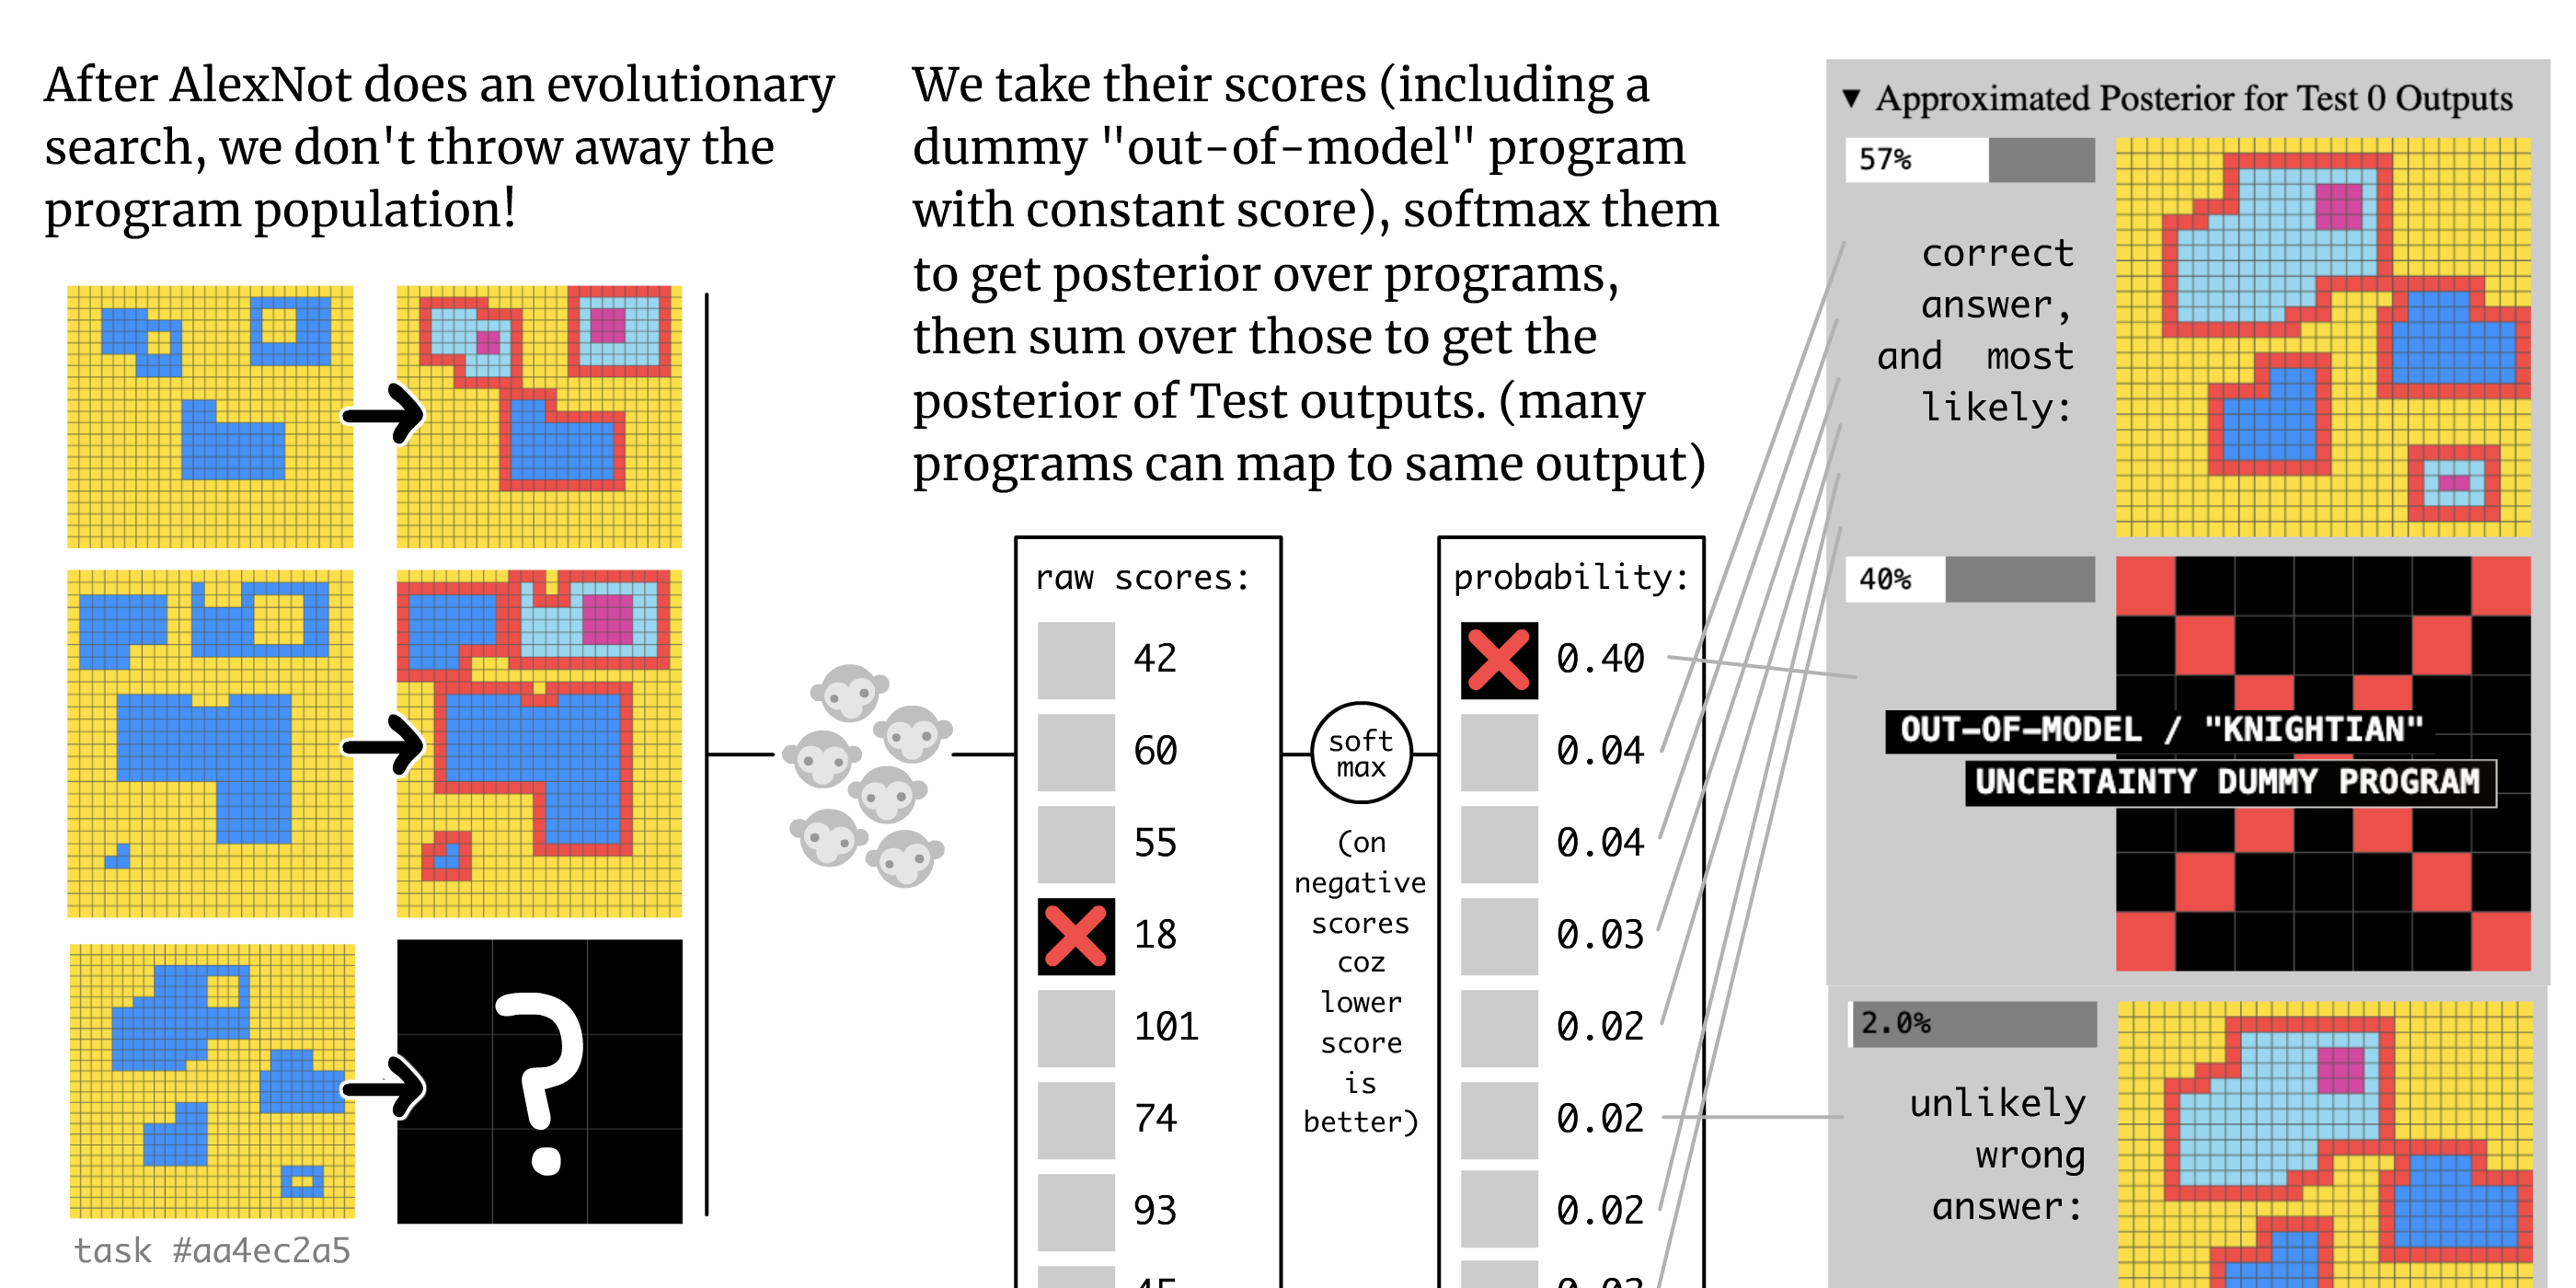
\includegraphics[width=\linewidth]{figures/across/bayes.png}
    \caption{Schematic of how AlexNot approximates a Bayesian posterior over programs \& Test outputs (with ``out-of-model''/pseudo-Knightian uncertainty).}
    \label{fig:alexnot_bayes}
\end{figure*}

So: compression is unreasonably effective\footnote{The title of this subsection is a riff off `The Unreasonable Effectiveness of Mathematics' \citep{wigner_math}. \mbox{(Non-)ironically}, compression may \textit{be} the answer why non-physical math is so effective in describing the physical world: math \textit{is} the ultimate compression, of all patterns we observe in reality, from numbers to spaces to symmetries.} in science, psychology, and AI. But \textit{why?}

In schematic pseudo-math, we can describe how good a compressed representation is, like so:\footnote{Note this implies we allow trade-offs, accepting a \textit{less} accurate model if it's much simpler! The `lossy compressions' of science. For example: Newtonian gravity (instead of full Einsteinian gravity), the Bohr model of the atom (instead of the full Schrödinger model), the water-and-pipes metaphor for electrical circuits.}
\[ \text{Compression} = \text{Simplicity} + \text{Accuracy} \]
Now consider (this simplified form of) Bayesian inference, the mathematically ideal way to learn from new data:
\[ \text{Posterior} \propto \text{Prior} \times \text{Likelihood} \]
If we set Simplicity = log(Prior), and Accuracy = log(Likelihood), then Compression = log(Prior) + log(Likelihood) = log(Prior x Likelihood) = log(Posterior) + a constant! To normalize all probabilities to sum to 1, take a softmax. \textbf{In sum: assuming a simplicity prior, softmaxxing on Compression \textit{is mathematically equivalent} to Bayesian inference, the ideal way to learn.}\footnote{To be clear: full Bayesian inference is usually intractable, so AlexNot only does a rough approximation.}

So, here's how we approximated that in AlexNot: (\autoref{fig:alexnot_bayes})

\begin{itemize}
    \item For each round of the evolutionary search, for each candidate program, we calculate its Simplicity and Accuracy metrics. Actually, no, for convenience, we score their \textit{opposites}: \textbf{Complexity and Error}. (more details below)
    \item The search selects programs with the lowest weighted-sum of Complexity + Error. (equivalently: highest Simplicity + Accuracy) For the sake of research minimalism, we just hard-coded the coefficient of the weighted sum. (Future research can make this a learned parameter, too.)
    \item At the end of the search, we have an importance-sampled list of candidates to approximate a Bayesian posterior. We simply softmax the scores to estimate, for each program, what's the probability this one is the true hidden rule?
    \item (Finally, because we can't evaluate \textit{all} possible programs, we mimic a Dirichlet process to estimate the \textbf{``out-of-model''/``unknown unknown'' uncertainty:} what's the probability the true program is one we \textit{didn't} evaluate? We do this by throwing in a `dummy program' with a fixed score into the softmax. Its only job is to take up probability-mass: the fewer simple/accurate programs the search finds, the higher probability the true hidden rule is one our search never even considered.)
\end{itemize}

But the devil's in the details, the power's in the priors. How \textit{specifically} did we operationalize `Error' and `Complexity'?

\subsection{Error (negative Accuracy)}

Let's start with Error, since it's more straightforward.

The most obvious way is to just add up the number of incorrectly-predicted pixels. (If the predicted \& ground-truth grids are different dimensions, all non-overlapping pixels count as incorrect.)

\begin{figure}
    \centering
    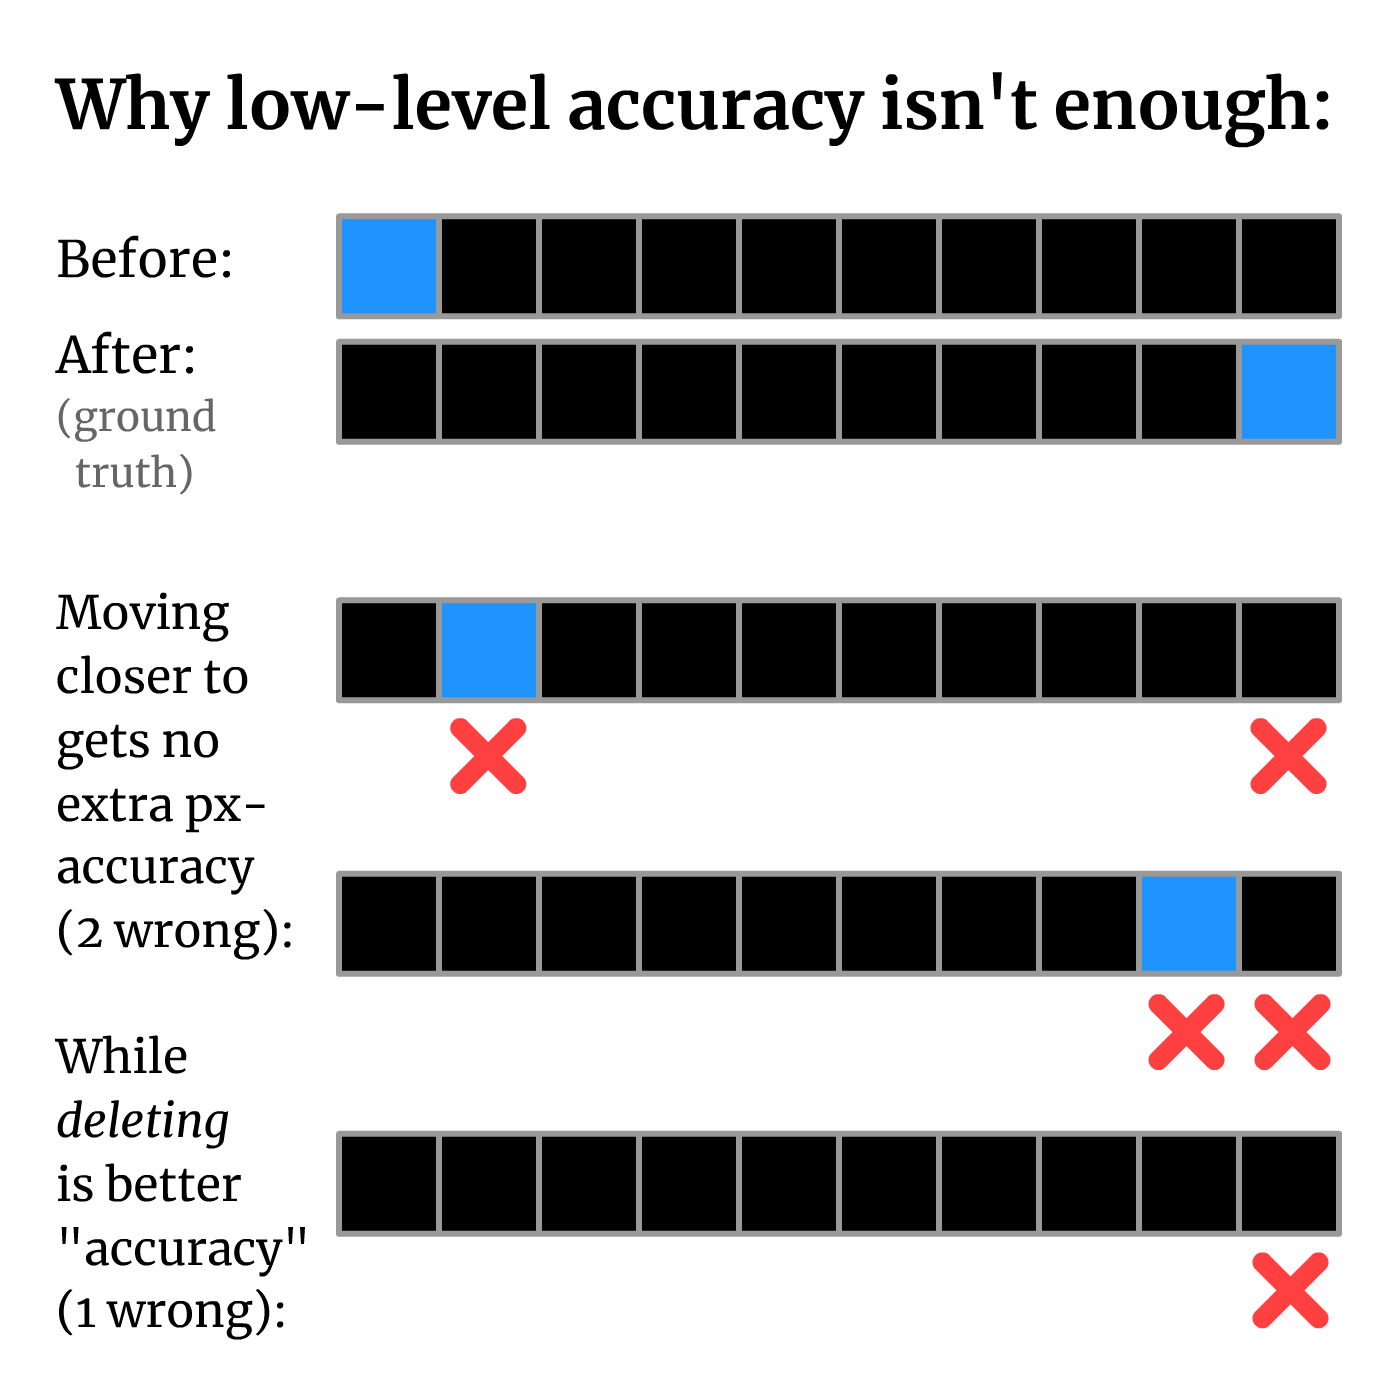
\includegraphics[width=\linewidth]{figures/mini/high_level.png}
    \caption{An example of how only paying attention to \textit{low-level} errors can lead a solver astray.}
    \label{fig:high_level_error}
\end{figure}

Later, we also found it helped to estimate error on high-level properties, like ``position of shape'' or ``missing/redundant shapes''. (\autoref{fig:high_level_error}) For concreteness, consider a blue 1px dot that's supposed to move from x=0 to x=10. Under the vanilla ``just add wrong pixels'' rule, predicting the blue dot at x=1 is \textit{just as good} as x=9: both result in 2 wrong pixels. In fact, \textit{deleting} the dot entirely is better: only 1 wrong pixel, at x=10. However, a smarter ``shape diff'' error estimator avoids this, and correctly marks x=9 as better than x=1, which is better than deleting the dot entirely. (Since ARC-AGI-1/2 requires pixel-perfect predictions, we used wrong-pixels as the final program selector, but shape-diff was a useful intermediary selection heuristic.)

In general, any good Compressor should pay attention to \textit{high-level} diffs, alongside \textit{low-level} diffs. This parallels a recent finding in neuroscience: ``prediction error'' signals fire in our brains, not just for low-level sensory predictions, but higher-level patterns, too! \citep{local_global_oddball,high_level_prediction_errors}

\subsection{Complexity (negative Simplicity)}

Let's start by just measuring \textbf{the length of the program}. This is the classic definition of algorithmic complexity, à la Kolmogorov Complexity or Minimum Description Length (MDL). Note: we count the number of \textit{tokens} in the program, so that `rotate' doesn't cost more than `fall', simply because English spells it with more letters.

Alas, this classic metric isn't enough, neither in practice nor in theory.

First off, Kolmogorov Complexity isn't even computable in principle.\footnote{To see this, consider Berry's Paradox: ``the smallest positive integer not definable in under eleven words'' (which is ten words long). \textit{If} Kolmogorov Complexity (length of the shortest program that can generate string X) was computable, you could make a similar paradoxical program: ``brute-force search all strings X in increasing-length order, such that Kolmogorov(X) >= N + 1'', where this program's length is N. A self-contradiction, therefore, Kolmogorov Complexity — and ideas that build on it, like Solomonoff Induction — \textit{can't} be computable, even in theory.}

Second, consider the following program: ``Loop through $0$ to $10^{1{,}000{,}000}$: convert this number to Unicode text, check if it's a complete valid Lean proof, save if yes, reject if no.'' This program \textit{would} decide every mathematical statement humanity ever could, and it \textit{is} one of the shortest programs to do so. There's just the \textit{teeny, tiny} problem that it'll take several Universe-ages to run. So, even though this is the most `compressed' program for superhuman math, it clearly doesn't match what we'd call `understanding'.

However, there's an easy fix! Consider not just the length of the program, but also \textbf{how much time the program takes}. (or any other `resource-bounded' metric, like memory space, or discrete actions taken.) Unlike Kolmogorov Complexity, resource-bounded complexity metrics like Levin Complexity \citep{levin_search} or the Speed Prior \citep{speed_prior} \textit{are} computable!\footnote{Why is (length+time) complexity computable, while plain Kolmogorov (just length) isn't? Because the paradoxical program in Kolmogorov requires \textit{indefinite} search; having any finite time constraint fixes that. Consider any string X. The program \texttt{print X} outputs X, and has length 6+|X|, time 1. Then you know \textit{as an upper bound} that the (length+time) complexity of X must be $7+|X|$. So, you can just try all programs of length 1 for $6+|X|$ steps, all programs length 2 for $5+|X|$ steps, all programs length 3 for $4+|X|$ steps, etc. This would be a \textit{very large} search, but crucially: it's \textit{finite}. It \textit{is} computable. (Levin Complexity does this, but with `dovetailing' and a time penalty of log(steps).)} This rules out brute-force methods like the above ``superhuman math AI''. And already, this concretely affects AlexNot's results. The intended solution is ``color shapes with 1 hole blue, 2 holes green, 3 holes red, 4 holes yellow''. However, if you only consider program length, and \textit{not} number of actions, the search might return ``color \textit{all shapes} blue, then recolor 2 holes green, 3 holes red, 4 holes yellow''. This \textit{is} a shorter program, but it unnecessarily paints every shape first. Regularizing against number of actions fixes this.
\begin{figure*}[b]
    \centering
    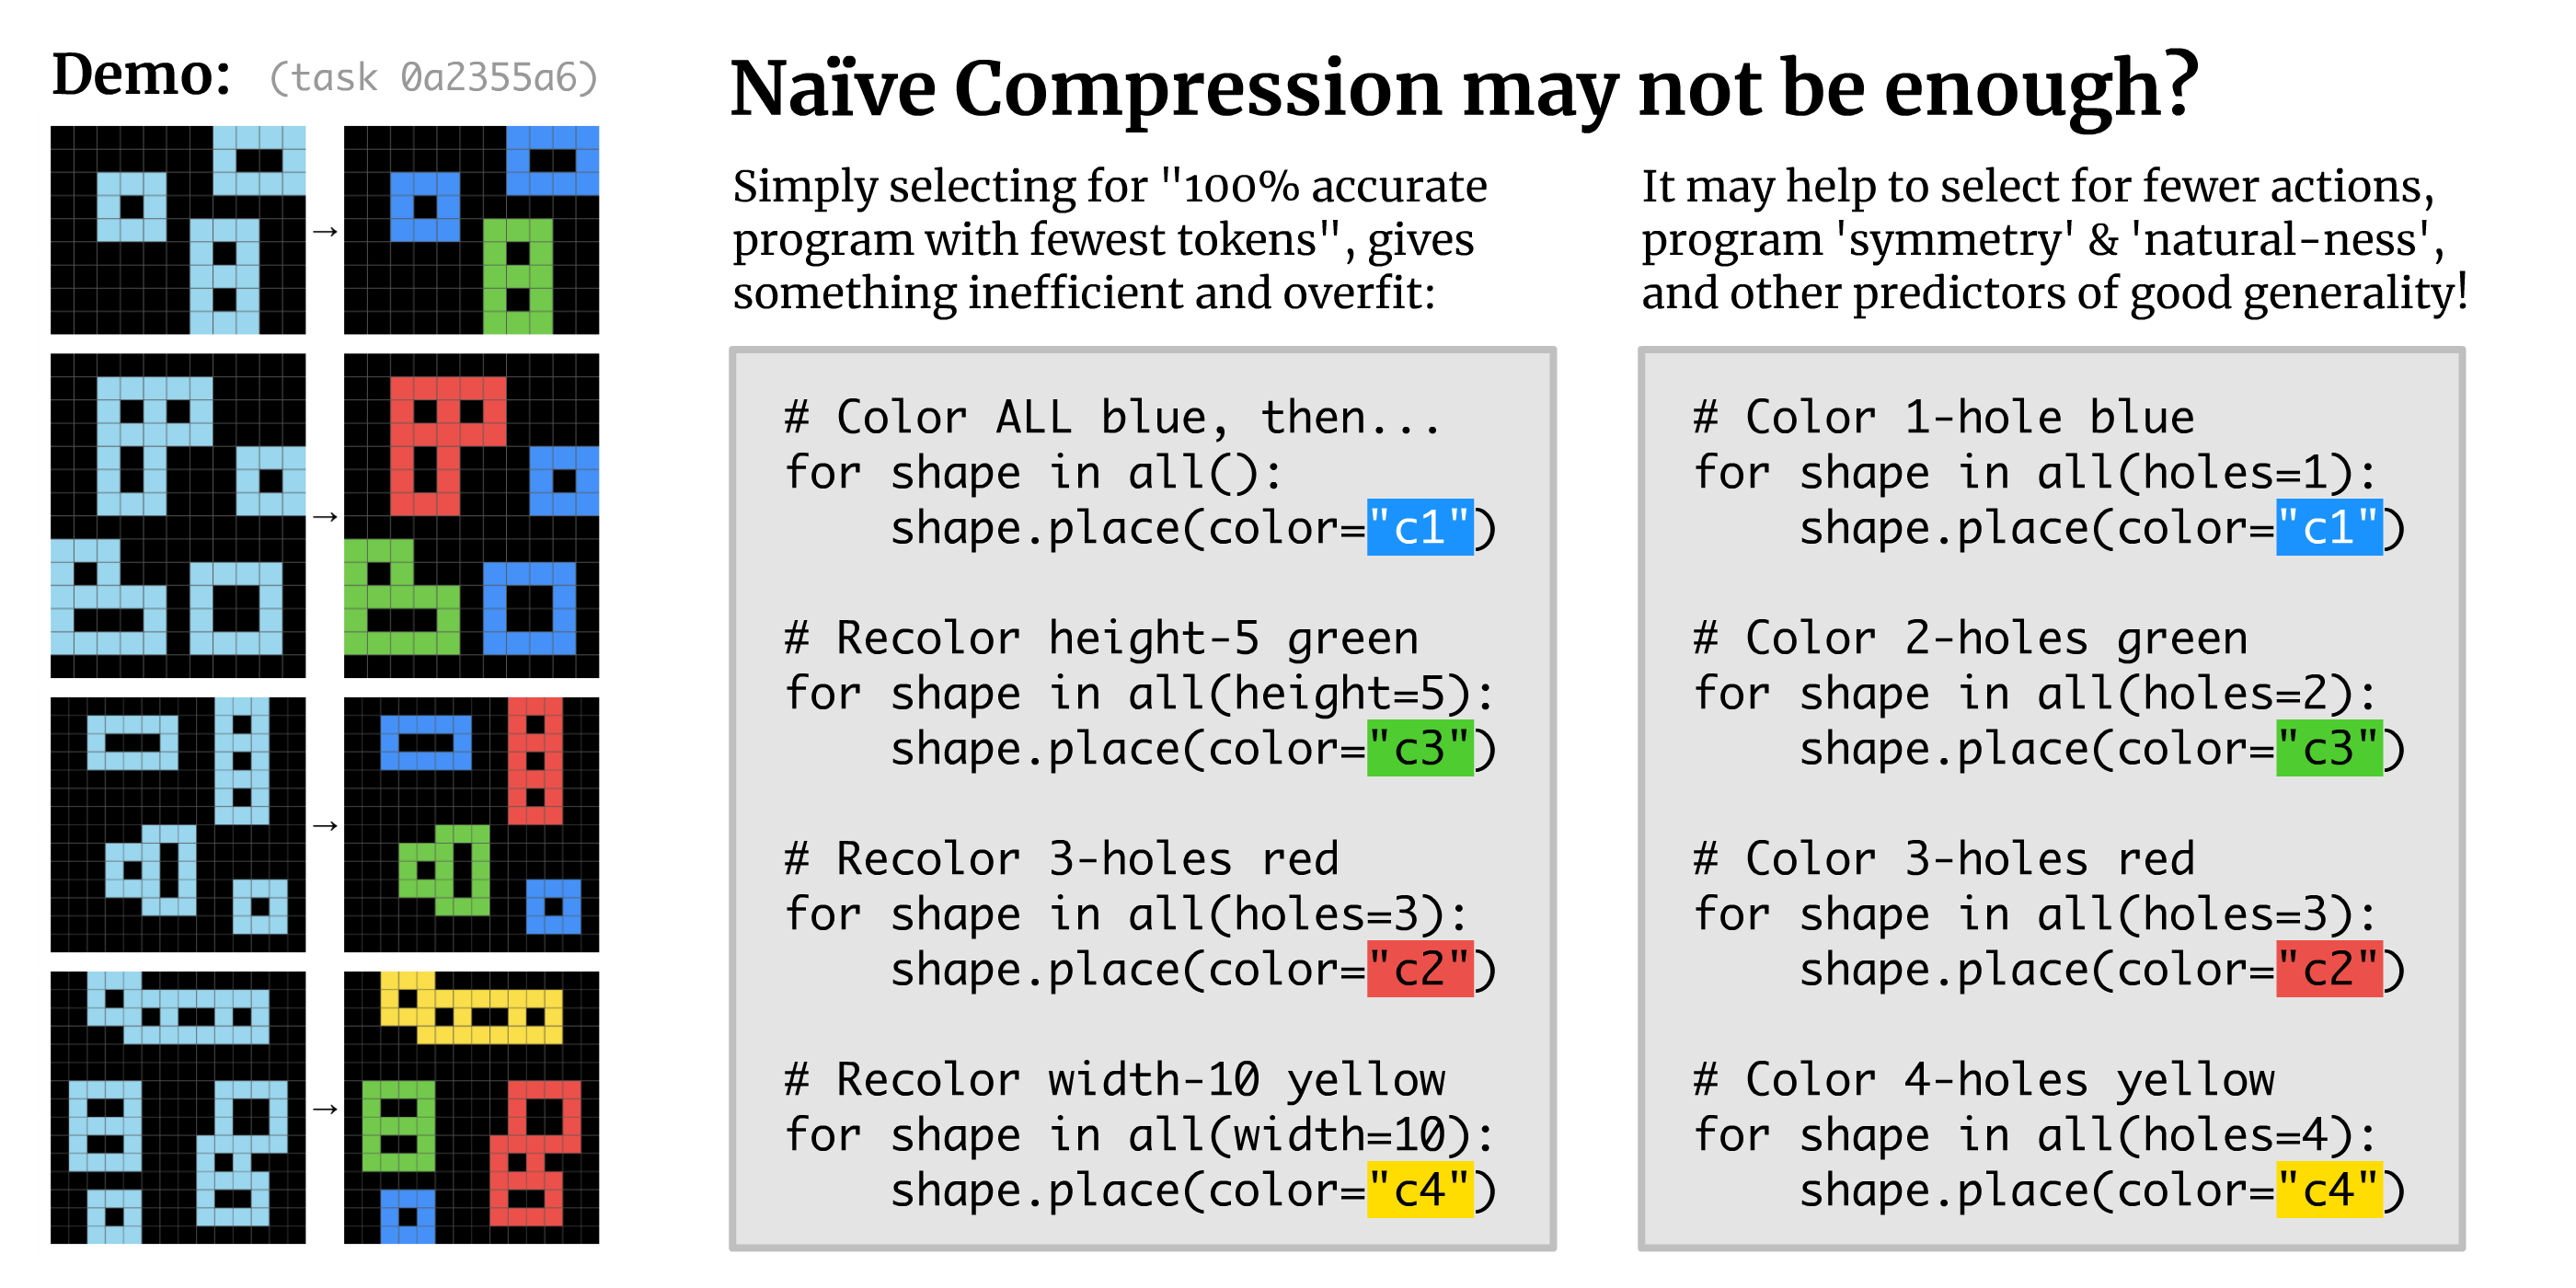
\includegraphics[width=\linewidth]{figures/across/beyond_compression.png}
    \caption{Example of where naïve compression leads a solver astray.}
    \label{fig:beyond_compression}
\end{figure*}

Actually, not quite. Even when penalizing unnecessary actions, the search can still give solutions no human would generate, like ``color shapes with 1 hole blue, \textit{height=5 green}, 3 holes red, \textit{width=10 yellow}.'' (See \autoref{fig:beyond_compression}.) To fix this, we penalize \textbf{how many \textit{unique} tokens/lines the program uses}, to incentivize re-using ideas \& concepts: ``symmetry'' in the program. (For future research: a more theoretically-grounded way of doing this, would be to measure the length of the program \textit{after} it's been compressed with grammar-based compression.)

In sum: while \textit{naïve} compression may fail, a smarter form of compression — rewarding not just fewer tokens, but also fewer concepts and fewer actions — could lead to solutions that don't just generalize better, but are more human-like, too! Compression Is All You Need!

\subsection{Compression Is \textit{Not} All You Need}

When we started this research project, we were sure — given the centuries-long throughline from Occam's Razor to Kolmogorov Complexity to the LLM–Compression connection — that simplicity would be all we needed. However, as ARC-AGI's own designer states in \citet{chollet_intelligence_efficiency}:
\begin{quote}
We do not expect that merely selecting the simplest possible program that works on training pairs will generalize well to test pairs. (cf. our definition of generalization difficulty)
\end{quote}
We found partial evidence for this! While iterating on AlexNot, we found it (slightly) helpful to add 3 more priors that don't quite fit under the banner of ``simplicity'':

\textbf{Fewer free parameters.} As von Neumann once said \citep{dyson_fermi_elephant}, \textit{``With four parameters I can fit an elephant, and with five I can make him wiggle his trunk.''} Consider a single demonstration of a 6-pixel shape moving 6 pixels up. Now consider two equally pixel-prediction-perfect programs: ``move all shapes 6 pixels up'' vs ``move all shapes up by its own area''. The first program is shorter, but the `fewer free parameters' rule picks the second, because it avoids the arbitrary `6' parameter. To punish arbitrariness, we simply penalize hard-coded literals.

\textbf{Bias towards invariant properties.} Given two equally-accurate, equally-short programs — like ``focus on the largest-\textit{area} shape'' vs ``focus on the largest-\textit{width} shape'' — we lean towards the first, since area stays invariant under flips \& rotations, while width doesn't. Invariant properties are more likely to generalize.

\textbf{Natural-ness.} It's easiest for humans to recognize 0 things vs 1 things. It's also easy to instantly recognize counts up to 4 things (`subitizing'). But it's harder to recognize 5 and up, and humans have to start manually counting. This is why, for AlexNot programs, the numbers 0/1 have the lowest penalty, 2/3/4 have small penalties, 5+ have the full penalty. More generally, we directly bias AlexNot towards human-psychology-compatible programs.\footnote{With two major exceptions: we do \textit{not} bias towards black backgrounds, even though that's more natural for humans, nor bias towards things falling downwards. This is because ARC's designers have stated that the color-digit mappings are intended to be arbitrary, and we got the (not-explicitly-stated) impression that ARC solvers should be invariant to grid orientation.}

You could argue the above are still related to `simplicity', but then you'd have to use a very \textit{not-simple} definition of simplicity. Let's step back: why select for a simplicity prior in the first place? Well, because ``find the simplest explanation'' has a good empirical track record of finding models that generalize. But if you're choosing `simple' for the sake of `generality', \textbf{isn't it simpler to select \textit{directly} for `generality'?} Then, simplicity becomes just one sub-metric of generality, on par with natural-ness and parameter-free-ness. And it makes evolutionary sense: of course our brains would be \textit{adapted to be adaptive}.

Alas, while ``select for accuracy + simplicity'' already has a common word — compression — ``select for accuracy + \textit{generalizability}'' does not. We couldn't find an exact match for this idea in the literature, but the closest idea is \textbf{condensation} \citep{eisenstat_condensation}. As \citet{demski_condensation} condenses it [emphases added]:
\begin{quote}
Condensation doesn't concern itself with the total code-length. Instead, it concerns itself with \textit{how easy it is to use the encoding to answer questions about the data}. [i.e. actual pragmatic usefulness.] This forces the encoding to be organized in a \textit{conceptually meaningful} way, rather than compressed together into an uninterpretable blob.
\end{quote}
So, contrary to the title of our own paper, perhaps it's not Understanding Is Compression, but Understanding Is \textit{Condensation}.

\subsection{Two More Simplicity-Priors: Language + Perception}

Since the following isn't the core of AlexNot, we'll compress (yuk yuk) our explanation of them. For full details, you can read our open-source code at \url{https://github.com/ncase/alexnot}, or ask an LLM to summarize it for you.

\begin{itemize}
    \item \textbf{The Domain Specific Language (DSL):} Language shapes our thoughts, thus, \textit{language is the biggest implicit prior}. To guard against overfitting to ARC-AGI, our DSL uses \textit{only} concepts that are plausible Core Knowledge Priors (even if not explicitly stated in \citet{core_knowledge_priors}): counting, sorting, causality, etc. This way, an otherwise 50-line Python program for move-down-with-collision-detection, gets condensed into a one \texttt{apply\_gravity()} line. Prior work: \citet{hodel_arc_dsl} made a DSL that covered all ARC-AGI-1 training tasks. Our DSL is simpler, more human-readable, and it's valid Python, so we can just use Python's exec function. Unfortunately, our DSL's biggest limitation is — unlike Hodel's DSL — ours does \textit{not} cover every ARC-AGI-1/2 train level, and isn't even Turing-complete. (To be discussed more in Limitations \& Future Research.)
    \item \textbf{Seeing Shapes:} To have programs that act on shapes, we must first parse the shapes from raw pixel grids. But what color should we assume the background is? Do diagonally-connected pixels count as part of the same shape? Do we try to re-use shapes between grids? There's a few hundred possible parser configurations, but that's small enough that we can just brute-force them all. We select the top parse that gives the simplest \textit{difference} between input and output scenes. To emphasize: not simplest \textit{scenes}, simplest \textit{difference} between scenes: parsings that require the fewest shape moves, recolors, deletions, creations, etc. (Formally, we select for lowest \textit{conditional} Kolmogorov Complexity, not lowest plain Kolmogorov Complexity.\footnote{Explanation: x=`0110101111' and y=`1001010000' both have high Kolmogorov complexity, because there's no simple program to generate x or y alone. However, x-given-y has low \textit{conditional} Kolmogorov complexity, because there's a simple program to generate x given y: just flip every bit! Note that in general, conditional Kolmogorov complexity is asymmetric.} More details to come in the next section, \hyperref[sec:search]{Problem-Solving is Search}.)
\end{itemize}

\subsection{Summary, Limitations, Future Research}

In summary, AlexNot seeks \textit{understanding}, by seeking \textit{compression} (or, ``condensation''). Programs are scored as a weighted sum of:

\begin{itemize}
    \item Accuracy: right pixels, right shape data
    \item Simplicity: fewer tokens, fewer \textit{unique} tokens/lines, fewer actions
    \item Generalizability: bias against hard-coded parameters, bias to invariance, bias to ``natural'' programs
\end{itemize}

Some limitations of our approach, and ideas for future research:

\begin{itemize}
    \item In obvious hindsight, if you want world models that generalize, you should select \textit{for generalization}. Simplicity is a part of that, and we found other aspects like ``natural-ness'', but there's no way we found them all. Future research should try precisely naming \& testing more predictors of generalization — and/or, train an ML/AI model to predict generalization. (But then, Catch-22: why should we expect \textit{that} generalization-predicting model to generalize?)
    \item Program scores were a weighted sum of various Accuracy, Simplicity, and Generalizability metrics, but the weights were chosen by hand. A future version could use ML to discover optimal weights, or better, use \textit{an ensemble} of weights. (Different Simplicity-to-Accuracy ratios map onto ``lumpers and splitters''.)
    \item Two promising priors we didn't try:
    \begin{itemize}
        \item a) Gricean maxims. \citep{grice_logic_conversation} If somebody shows you an exercise ball with a face and two antennae, and says, ``this is a Space Hopper'', you'd induce ``A Space Hopper is an exercise ball with a face and two antennae'', even though the \textit{simplest} model that predicts all N=1 samples would be ``\textit{Anything} is a Space Hopper.'' The fact that we can learn definitions from \textit{a single positive example} shows the power of Gricean maxims: we fruitfully assume that when one agent tries to teach another, they'll do so in an efficient manner.
        \item b) Causal plausibility. As xkcd 1122\footnote{\url{https://xkcd.com/1122/}} noted, all 56 U.S. presidential elections up to 2012 could be perfectly explained by a simple rule: ``Democratic incumbents never beat taller challengers.'' While this definitely ``compresses'' all N=56 data points, it's obviously overfit nonsense. An AI that condenses real-world knowledge into world models should \textit{explicitly} select for plausible causal mechanisms.
    \end{itemize}
    \item Our DSL does \textit{not} cover all ARC-AGI levels, isn't even Turing-complete, and making the DSL manually was a pain in the [rejected by reviewer 2]. An ideal AI should be able to \textit{grow its own DSL}. And this DSL should be fully human-interpretable: each new `concept' is a program that calls previous concepts, all the way down to the primitives. In the \hyperref[sec:limitations]{Future Research} section, we sketch out a design for a DreamCoder+LLM+AlexNot neuro-symbolic system that does this.
    \item Since ARC-AGI-1/2 uses pixel-perfect data, AlexNot only seeks \textit{lossless} compression. But real-world data has noise, so we need good \textit{lossy} compressions. In \hyperref[sec:results]{Results \& Experiments}, we'll present a proof-of-concept for AlexNot inducing real-world differential equations, from noisy, sparse time-series data. Stay tuned!
\end{itemize}




\begin{figure*}
    \centering
    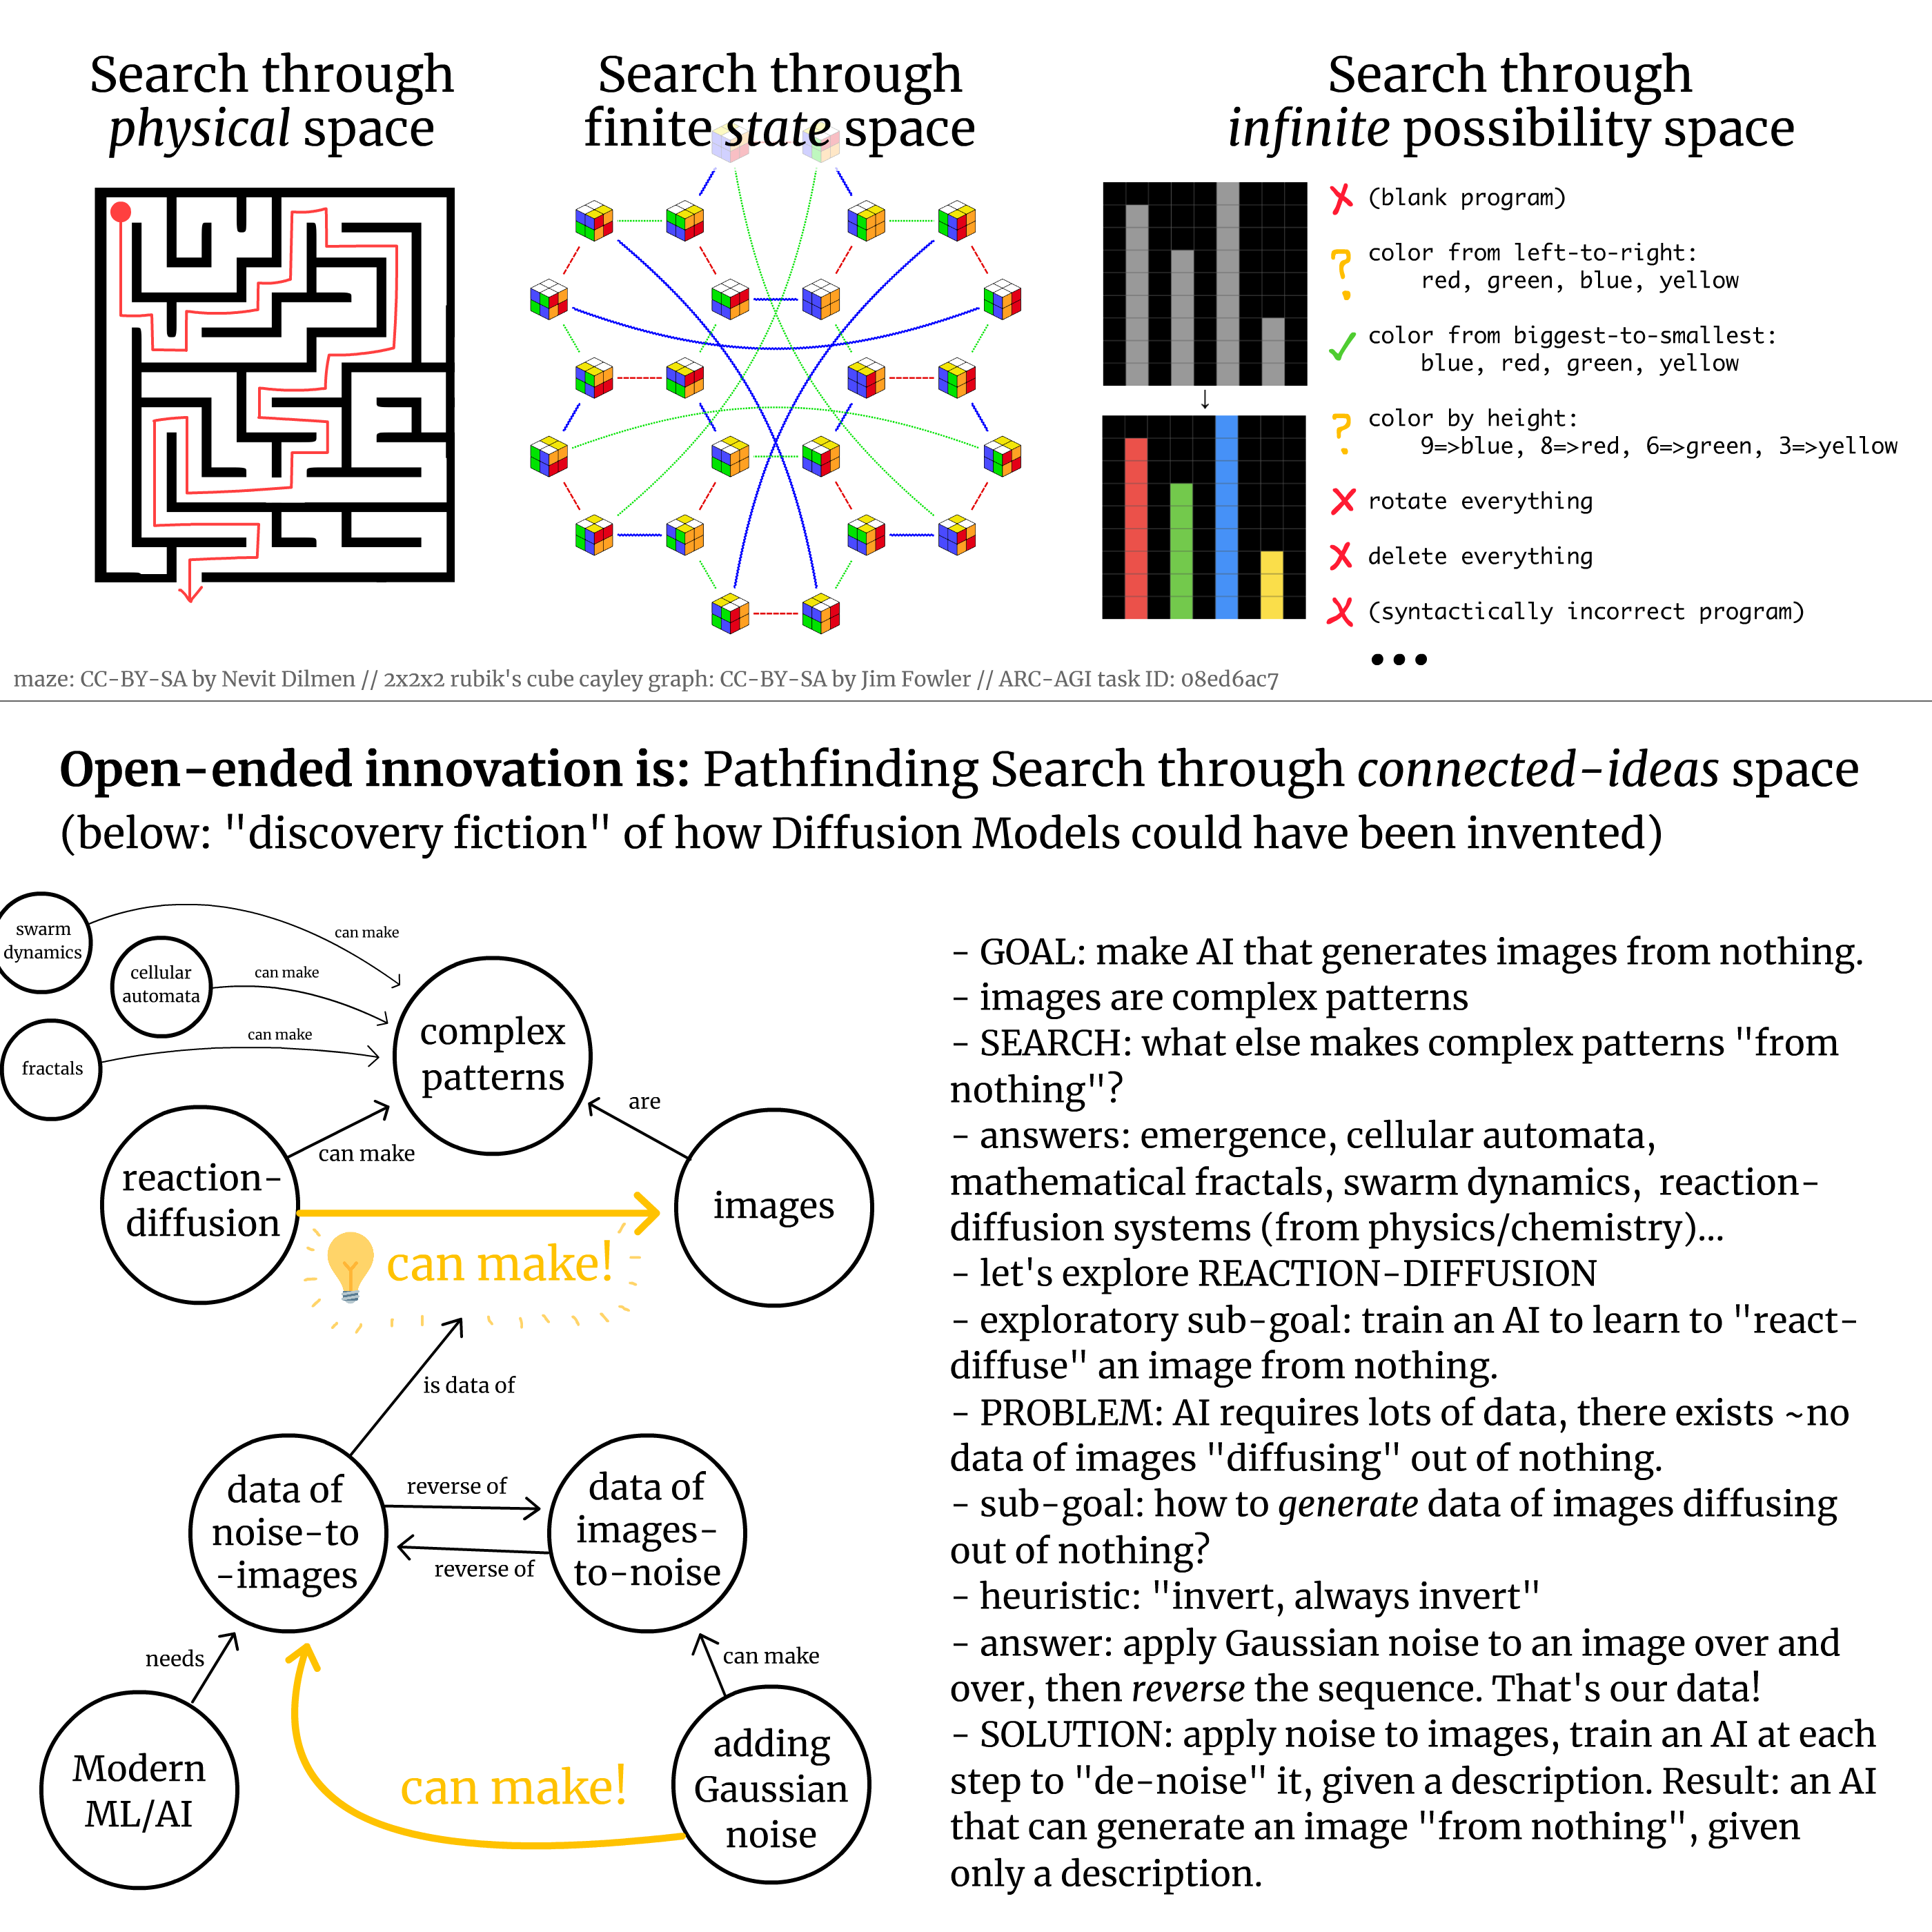
\includegraphics[width=\linewidth]{figures/across/search.png}
    \caption{Examples of problem-solving as search. (a) Maze (b) Rubik's cube (2x2x2), (c) ARC-AGI task, (d) \textit{Open-ended innovation}. Here, we present a `discovery fiction' of how diffusion models could have been invented.}
    \label{fig:problem_solving}
\end{figure*}



%%%%%%%%%%%%%%%%%%%%%%%%%%%%%%%%%%%%%%%%%%%%%%%%%%%%%%%%%%%%%%%%%%%%%%%%%%%%%%%%%%%%%%
%%%%%%%%%%%%%%%%%%%%%%%%%%%%%%%%%%%%%%%%%%%%%%%%%%%%%%%%%%%%%%%%%%%%%%%%%%%%%%%%%%%%%%
% PROBLEM-SOLVING IS SEARCH
%%%%%%%%%%%%%%%%%%%%%%%%%%%%%%%%%%%%%%%%%%%%%%%%%%%%%%%%%%%%%%%%%%%%%%%%%%%%%%%%%%%%%%
%%%%%%%%%%%%%%%%%%%%%%%%%%%%%%%%%%%%%%%%%%%%%%%%%%%%%%%%%%%%%%%%%%%%%%%%%%%%%%%%%%%%%%

\section{Problem-Solving is Search}\label{sec:search}

\subsection{Search me}

``Problem-Solving is Search'' is an old principle in AI: Newell, Shaw \& Simon's \textit{General Problem Solver} \citep{general_problem_solver} was created on the belief that almost all\footnote{Excluding `problems' that are purely mechanical rote, no choice required: multiplying large numbers, solving linear equations, etc.} problems we care about can be reframed as \textit{a search problem:} through literal space, state space, infinite combinatoric space, or through the space of ideas themselves. (See \autoref{fig:problem_solving}) Let's linger on that last one, because \textbf{open-ended innovation} is what the to-be-revealed ARC-AGI-4 will target, and advancing scientific \& technological innovation is the whole \textit{reason} to make AGI in the first place.

In the above Figure, we show a ``discovery fiction'' \citep{nielsen_discovery_fiction} for how image-generating diffusion models \citep{sohl_dickstein_diffusion,ddpm} \textit{could} have been invented via a search through a concept-graph. Let's go further, and tackle Demis Hassabis's ``Einstein Test'' \citep{hassabis_lex_fridman}, paraphrased: \textit{could an AI, with knowledge only up to 1900, re-derive General Relativity?} This is also the same example used in the position paper, \textit{LLMs Can't Jump} \citep{llms_cant_jump}. Here's a possible path through connected-idea space, of how \textit{you} could have made the abductive ``jump'' to discovering General Relativity:
\begin{quote}
Daydreaming: Bored at a Swiss patent office. Imagine a guy falling off a roof. $\to$ Connection: When you fall, you feel weightless. $\to$ Connection: Weightless means no acceleration, an inertial frame. $\to$ \textit{Contradiction!} \textit{Problem found.} Things in inertial frames move in straight lines, yet things fall in curves! How can this be? $\to$ Search for analogy: what else is both straight yet curved? $\to$ Connection: geodesics in curved space, like lines of longitude on a globe; lines parallel at the equator come together at the poles, \textit{as if by attractive force}. $\to$ New Hypothesis! Gravitational pull is actually things moving in `straight lines' \textit{on a curved spacetime.} $\to$ Next Action: beg your ol' college buddy Marcel Grossmann for a crash course in Riemannian geometry.
\end{quote}
Note that breakthroughs like Einstein's aren't just problem-solving, but also \textbf{problem-finding}. Any child who's jumped off a swing knows you feel weightless while falling, but Einstein was one of the first few to consider it a \textit{problem}, and actually solve it.

Thankfully, ``finding fruitful problems'' is itself just a problem, which can be tackled with search heuristics, such as these prompts for creating \textit{new} connections:

\begin{itemize}
    \item \uline{Notice contradictions}: ``Huh, that's odd... if parents' traits blend together, why does crossbreeding purple flowers with white flowers \textit{not} make grandkids that are 100\% light-purple, but instead, they're 75\% full-purple and 25\% full-white?'' $\to$ Gregor Mendel's discovery that inheritance comes in discrete chunks (`genes').
    \item \uline{Notice coincidences}: ``Huh, that's odd... South America's coastline looks really similar to Africa's...'' $\to$ Alfred Wegener's discovery of continental drift.
    \item \uline{Notice happy accidents}: ``Huh, that's odd... this Petri dish I accidentally left out has no bacterial growth around this mold...'' $\to$ Alexander Fleming's discovery of penicillin.
    \item \uline{Break a rule}: ``What if you \textit{could} take the square root of a negative number?'' $\to$ imaginary \& complex numbers. ``What if you \textit{could} meaningfully say `infinity plus one'?'' $\to$ hyperreal numbers.
    \item \uline{Try doing an old thing in a new way}: ``What if you did geometry with \textit{algebra}?'' $\to$ Descartes’ coordinate geometry.
    \item \uline{Try doing a new thing in an old way}: ``What if I tackled ARC-AGI with good ol' fashioned AI \& classic cognitive science theory?'' $\to$ this paper! :)
    \item \uline{Daydreaming}: Einstein imagined a man falling off a roof. Schrödinger imagined a dead cat in a box. Foot imagined killing one guy with a trolley to save five. \sout{Maybe a genius AI should constantly fantasize about murder} Open-ended innovation comes from ``daydreaming'' random inputs, and seeing what connections grow from there.
\end{itemize}

We apologize for belabouring the point, but we \textit{really} want to hammer it home: we suspect the key to unlocking open-ended innovation in AI — even Einstein-level ``jumps'' — is `just' \textbf{efficient search over paths through connected-idea space}, both to solve problems and \textit{find} problems. (For evidence of this claim: see how ``Knowledge Graphs'' are already quietly helping with real-world drug discovery \citep{kg_drug_discovery_review}, including finding a Covid-19 treatment in weeks, later FDA emergency-approved! \citep{baricitinib_kg,baricitinib_kg_method})

And as the above examples show, these idea-paths aren't even long, just a few connected hops! That's low search \textit{depth}, but the challenge is search \textit{width}: if there's a million facts, there's a million-million possible connections between facts. This combination — low depth, high width — is what makes genius seem ``obvious in hindsight''. \textit{Finding} the path is hard, \textit{following} an already-found path is easy.

\subsection{How does the human brain implement search?}

From the astronaut's-eye view, a wide range of search algorithms — from A* to evolutionary search — are fundamentally the same thing: select best candidates, tweak them to generate new candidates, repeat.

Many cognitive scientists, over many decades, have independently converged on the same general idea for how the human brain implements this: (\autoref{fig:gwt})

\begin{figure}[H]
    \centering
    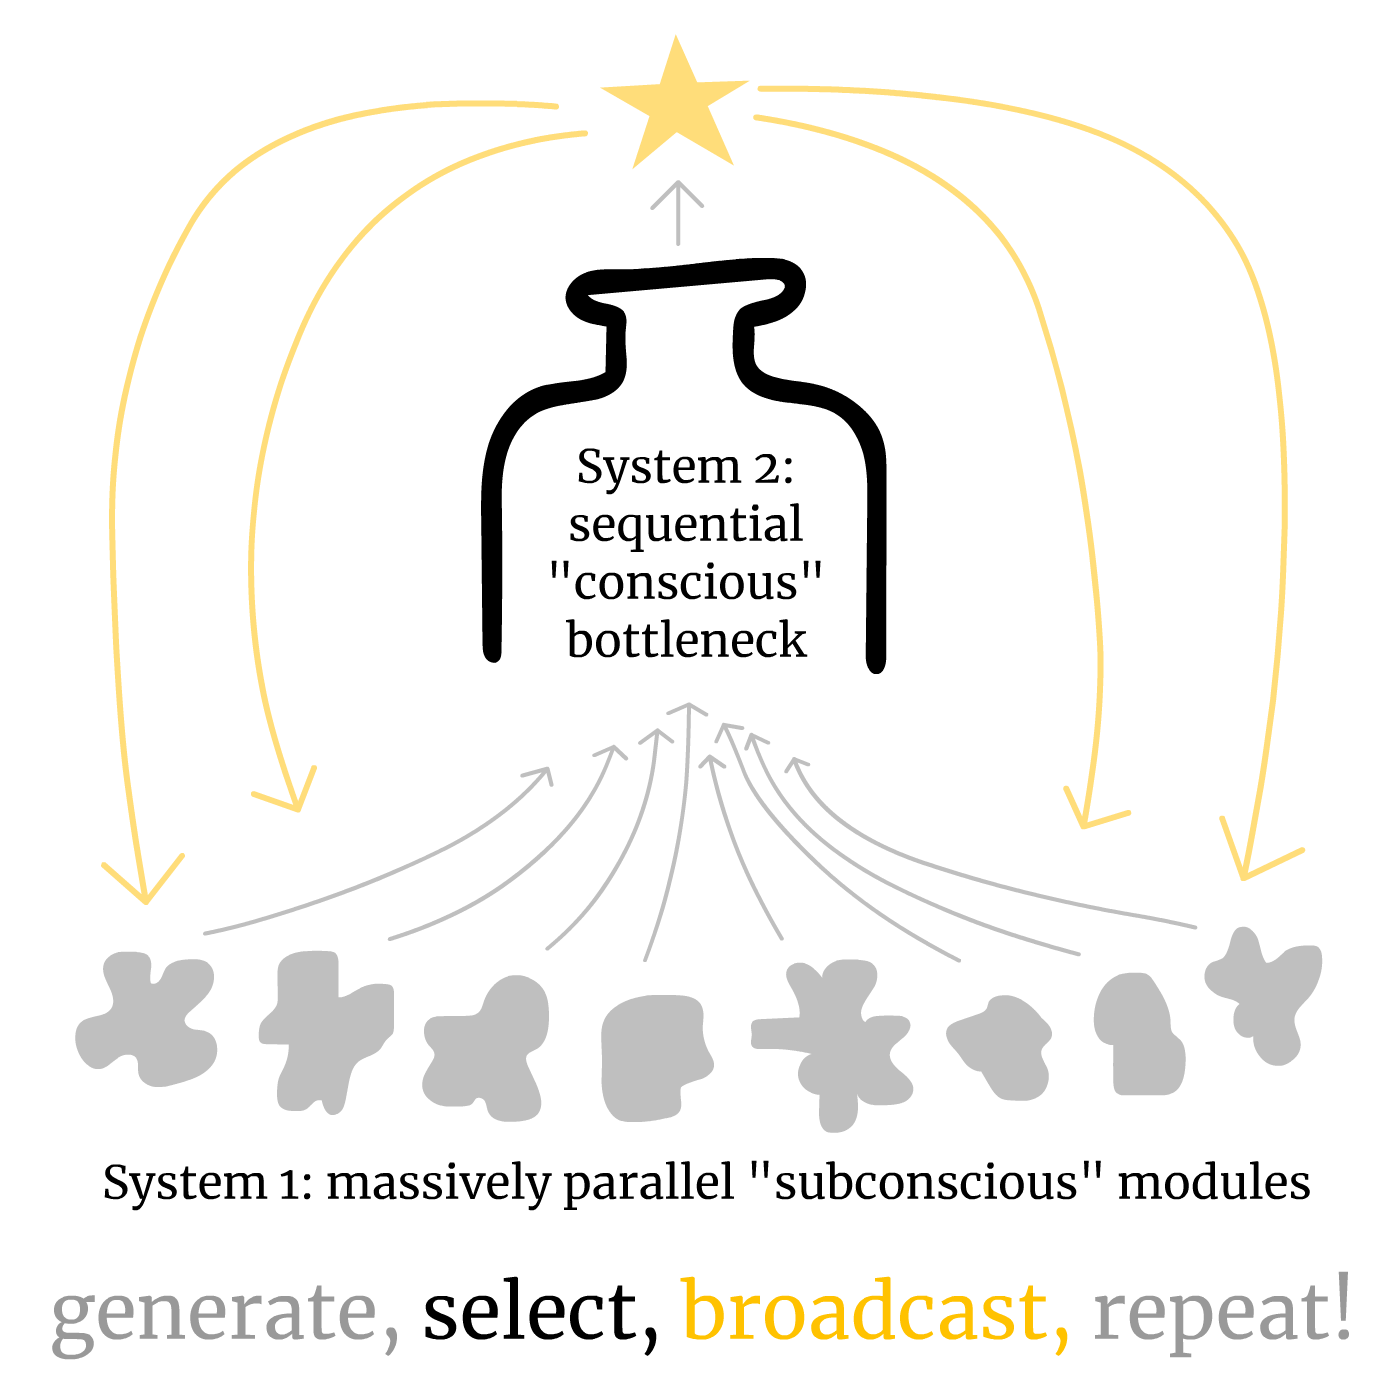
\includegraphics[width=\linewidth]{figures/mini/gwt.png}
    \caption{The `converged model' of how the mind works.}
    \label{fig:gwt}
\end{figure}

\begin{enumerate}
    \item a \textbf{slow, sequential bottleneck} selects a few thoughts at a time (System 2/consciousness)
    \item then broadcasts these thoughts to a vast array of \textbf{fast, parallel modules} (System 1/subconscious)
    \item which generate new candidate thoughts
    \item then the highest-salience/most-important ones are selected \& re-broadcast to all
    \item repeat!
\end{enumerate}

Proposals in this vein include: \textit{Pandemonium} \citep{pandemonium}, \textit{Blackboard} \citep{hearsay_blackboard}, \textit{Society of Mind} \citep{society_of_mind}, \textit{Fame in the Brain} \citep{sweet_dreams}, \textit{System 1 and System 2} \citep{thinking_fast_and_slow}, the \textit{Consciousness Prior} \citep{consciousness_prior}, and the leading neuroscience-backed theory of consciousness, \textit{Global Workspace Theory} (GWT) \citep{baars_gwt}.

(\textit{To be clear,} A $\to$ B $\neq$ B $\to$ A. Just because the computational job of consciousness is to integrate \& re-broadcast diverse information, does not (necessarily) mean that \textit{any} system that does the same job is conscious. If that were the case, \textit{the U.S. stock market} would be conscious (cf.\ \citealp{schwitzgebel_us_conscious}), and in fact, \textit{more} conscious than a human being.\footnote{\citet{unbearable_slowness} estimates ``the information throughput of a human being is about \textbf{10 bits/s}''. In contrast, \textit{very} conservatively assuming that each stock update is 1 bit (up/down), and stocks update on average once a minute, and there's 4,000 listed companies on the US stock exchange, that's still 4,000 bits/minute or \textbf{67 bits/s}: \textit{seven times more} than human conscious processing.} Perhaps there's another way current or future AI could be conscious — especially ones using neuromorphic hardware \citep{neuromorphic_review} or \textit{real biological human neurons} grown on microchips \citep{dishbrain} — but this is not a philosophy paper, so we'll shut up now.\footnote{Except to say: even if AI can never be conscious, please don't be cruel towards realistic person-shaped entities, for your \textit{own} sake — as Kurt Vonnegut once warned, \textit{``We are what we pretend to be, so we must be careful about what we pretend to be.''}})

Arguably, the above is how LLMs work, too: a large neural network can be thought of as an ensemble of massively parallel sub-networks — this implicit ensemble is explicit in Mixture of Experts models — and the ``bottleneck'' is the softmax which picks 1 token at a time, then all previously-chosen tokens are re-broadcast to all sub-networks, repeat. (Related: there's some early evidence of a Global Workspace-like space inside LLMs! \citep{llm_global_workspace}) We'll expand more on this idea in the \hyperref[sec:limitations]{Future Research} section, in our design sketch for a DreamCoder+AlexNot+LLM harness.

\subsection{So how does AlexNot implement search?}

We use a \textit{guided} evolutionary search, to implement the above GWT-like idea: a small bottleneck of chosen programs, iterated upon by a wide array of parallel modules, repeat.

(This is \textit{not} a new approach, in program synthesis or even in ARC-AGI. FunSearch \citep{funsearch} and AlphaEvolve \citep{alphaevolve} use LLMs as the intelligent program-editing heuristics in an evolutionary search for general coding tasks; Jeremy Berman used Grok 4 in an evolutionary search to achieve a score of 29.4\% on ARC-AGI-2 \citep{berman_arc_english}. What \textit{is} novel about our approach, is that \textit{even our heuristics} are pure-symbolic. And while we do get a lower score than LLM-guided approaches, it's still on par with last year's Top 3 results, but over 5,000$\times$ cheaper.)

Anyway, here's the core AlexNot loop, a search for the best ``transform'' program:

\begin{enumerate}
    \item Start with the ``empty'' program. It does nothing.
    \item Take \{the current pool of programs, their predictions, and all Demo pairs\}, and \textbf{broadcast them to \textit{all} code-proposing modules, which we call ``monkeys''}.\footnote{To evoke the idea of `code monkey', `evolution', `monkey-see-monkey-do', and `millions of monkeys on typewriters'.}
    \begin{itemize}
        \item Each monkey is responsible for one (1) Core Knowledge Prior — a ``rotation monkey'', a ``coincidence monkey'', etc — and can each propose up to 100s of possible candidate programs.
        \item Most monkeys are execution-guided \citep{execution_guided}: they use \textit{the difference} between a program's prediction \& ground-truth output (its \textit{prediction error}) to propose how to edit the program. For example, a monkey notices a red square should be further down than predicted, so it proposes dozens of additions: \textit{move red down, red falls down, move squares down, square falls down,} etc.
    \end{itemize}
    \item \textbf{Select the best new-candidate programs}, using the Accuracy + Simplicity + Generalizability metrics described in the above section, Understanding Is Compression.
    \begin{itemize}
        \item To encourage program diversity, we select as parents: the best program on \textit{all} Demo pairs + the best program on just Demo 0 + the best program on just Demo 1 + (and so on) + the best program on all Demo pairs \textit{only considering shape-diff}, not pixel-diff. This is an ``island-model'' or ``Galapagos'' evolutionary search \citep{island_model}, with all-to-all migration every round. This way, if the search ever gets stuck on a local minimum on one island, it can continue exploration on at least one other island, then spread.
    \end{itemize}
    \item Repeat until time's up, or a better-scoring program isn't found for 2 more rounds.
\end{enumerate}

By the end, we get not just one, but a whole \textit{population} of candidate programs. For each Test, the \#1 best gets applied as Attempt 1, and Attempt 2 is the next-best program that generates a pixel-different output.

. . .

\begin{figure*}
    \centering
    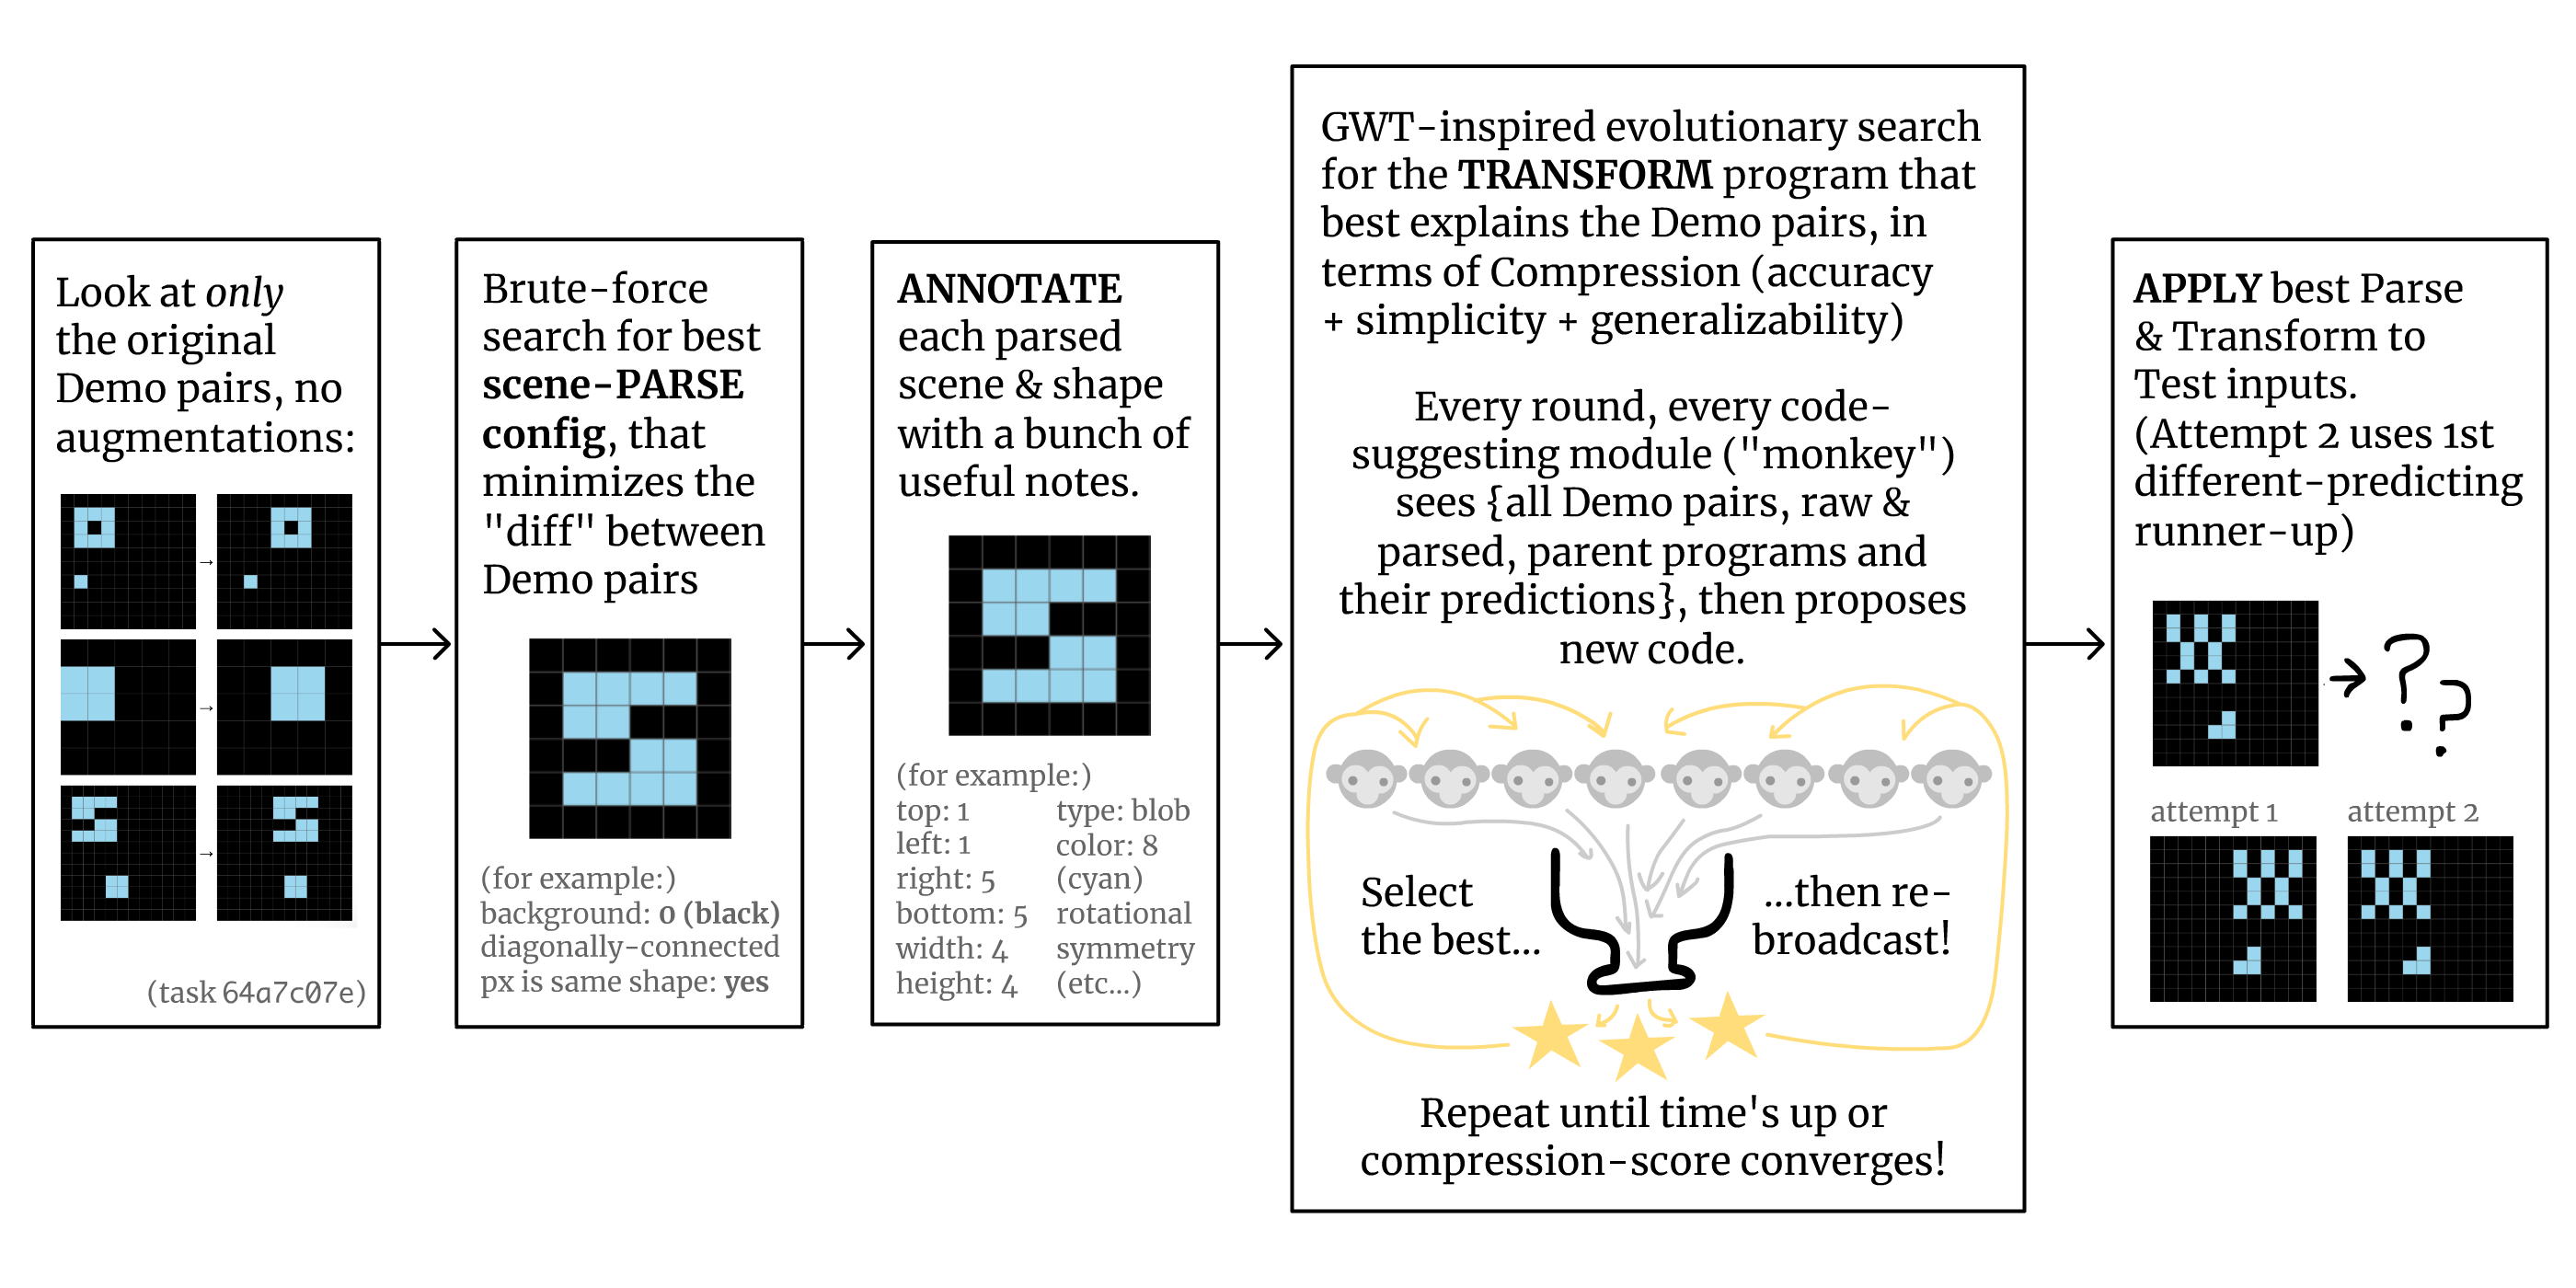
\includegraphics[width=\linewidth]{figures/across/alexnot_full.png}
    \caption{The \textit{full} schematic for how AlexNot works: Parse, Annotate, Transform, Apply.}
    \label{fig:alexnot_full_schematic}
\end{figure*}

Okay, we skipped some detail. Let's back up. \textit{Before} the above ``how to transform shapes'' search can run, we need to figure out how to \textbf{parse} shapes in the first place, from the pixel grids. (e.g. what color's the background, do diagonally-connected pixels count as part of the same shape? etc.) Thankfully, the possibility space is only in the low hundreds, so we just brute force them all, and pick the one that leads to the simplest \textit{difference} between the before/after scenes. ($\approx$\textit{conditional} Kolmogorov Complexity.)

Next, we \textbf{annotate} each shape with a bunch of useful properties the search can use, like ``this shape's color'' or ``how many other shapes share the same silhouette'' or ``this shape has the Nth biggest area'', etc.

Only \textit{then} do we search for the best \textbf{transform}, then apply it to the \textbf{test}. See \autoref{fig:alexnot_full_schematic} for the \textit{full} AlexNot solver schematic.

. . .

Okay, there's actually \textit{one} more important search that AlexNot does: \textbf{causality}. Whenever a code-monkey proposes something like, ``all shapes with X,Y properties get flipped'', it first has to find out: what properties do all the flipped-shapes have in common, that \textit{none} of the non-flipped shapes have? This is similar to Bongard Problems \citep{bongard_problems}: what rule separates the positive \& negative examples? Thankfully, each shape only has a couple dozen properties, so there's < 1000 possible 1-property and 2-property separators to test. (We do not attempt 3 or more properties.) So, we just brute-force them all to find what works as separators. This ``Causality/Bongard'' search runs 100s of times per puzzle: for each round of evolution, for each code-monkey.

\subsection{Only a fool plays with one hypothesis}

When it comes to AIs that induce world models from data, it's crucial they keep \textit{a whole approximate Bayesian distribution} of solutions, not just the best one. This lets an AI ``know what it doesn't know'', which is crucial for both AI capabilities \textit{and} safety. (See the previous section \hyperref[sec:compression]{Understanding is Compression}, especially \autoref{fig:alexnot_bayes}, for how we approximate a Bayesian distribution over programs \& predictions in AlexNot. To recap: we keep the whole population from the evolutionary search, then softmax over their scores to get a probability distribution, with a ``out-of-model'' dummy entry, to estimate the probability the true answer is one it doesn't know.)

\textbf{For AI Capabilities:} by maintaining uncertainty, an AI can better balance exploring \& exploiting novel environments. For AI-driven science, it lets you do ``optimal experiment design'' \citep{lindley_experiment_information,chaloner_bayesian_design}: given a probability distribution of possible worlds, what experiment will give you the most expected information, \textit{distinguishing} between possible worlds?
\begin{figure*}[t]
    \centering
    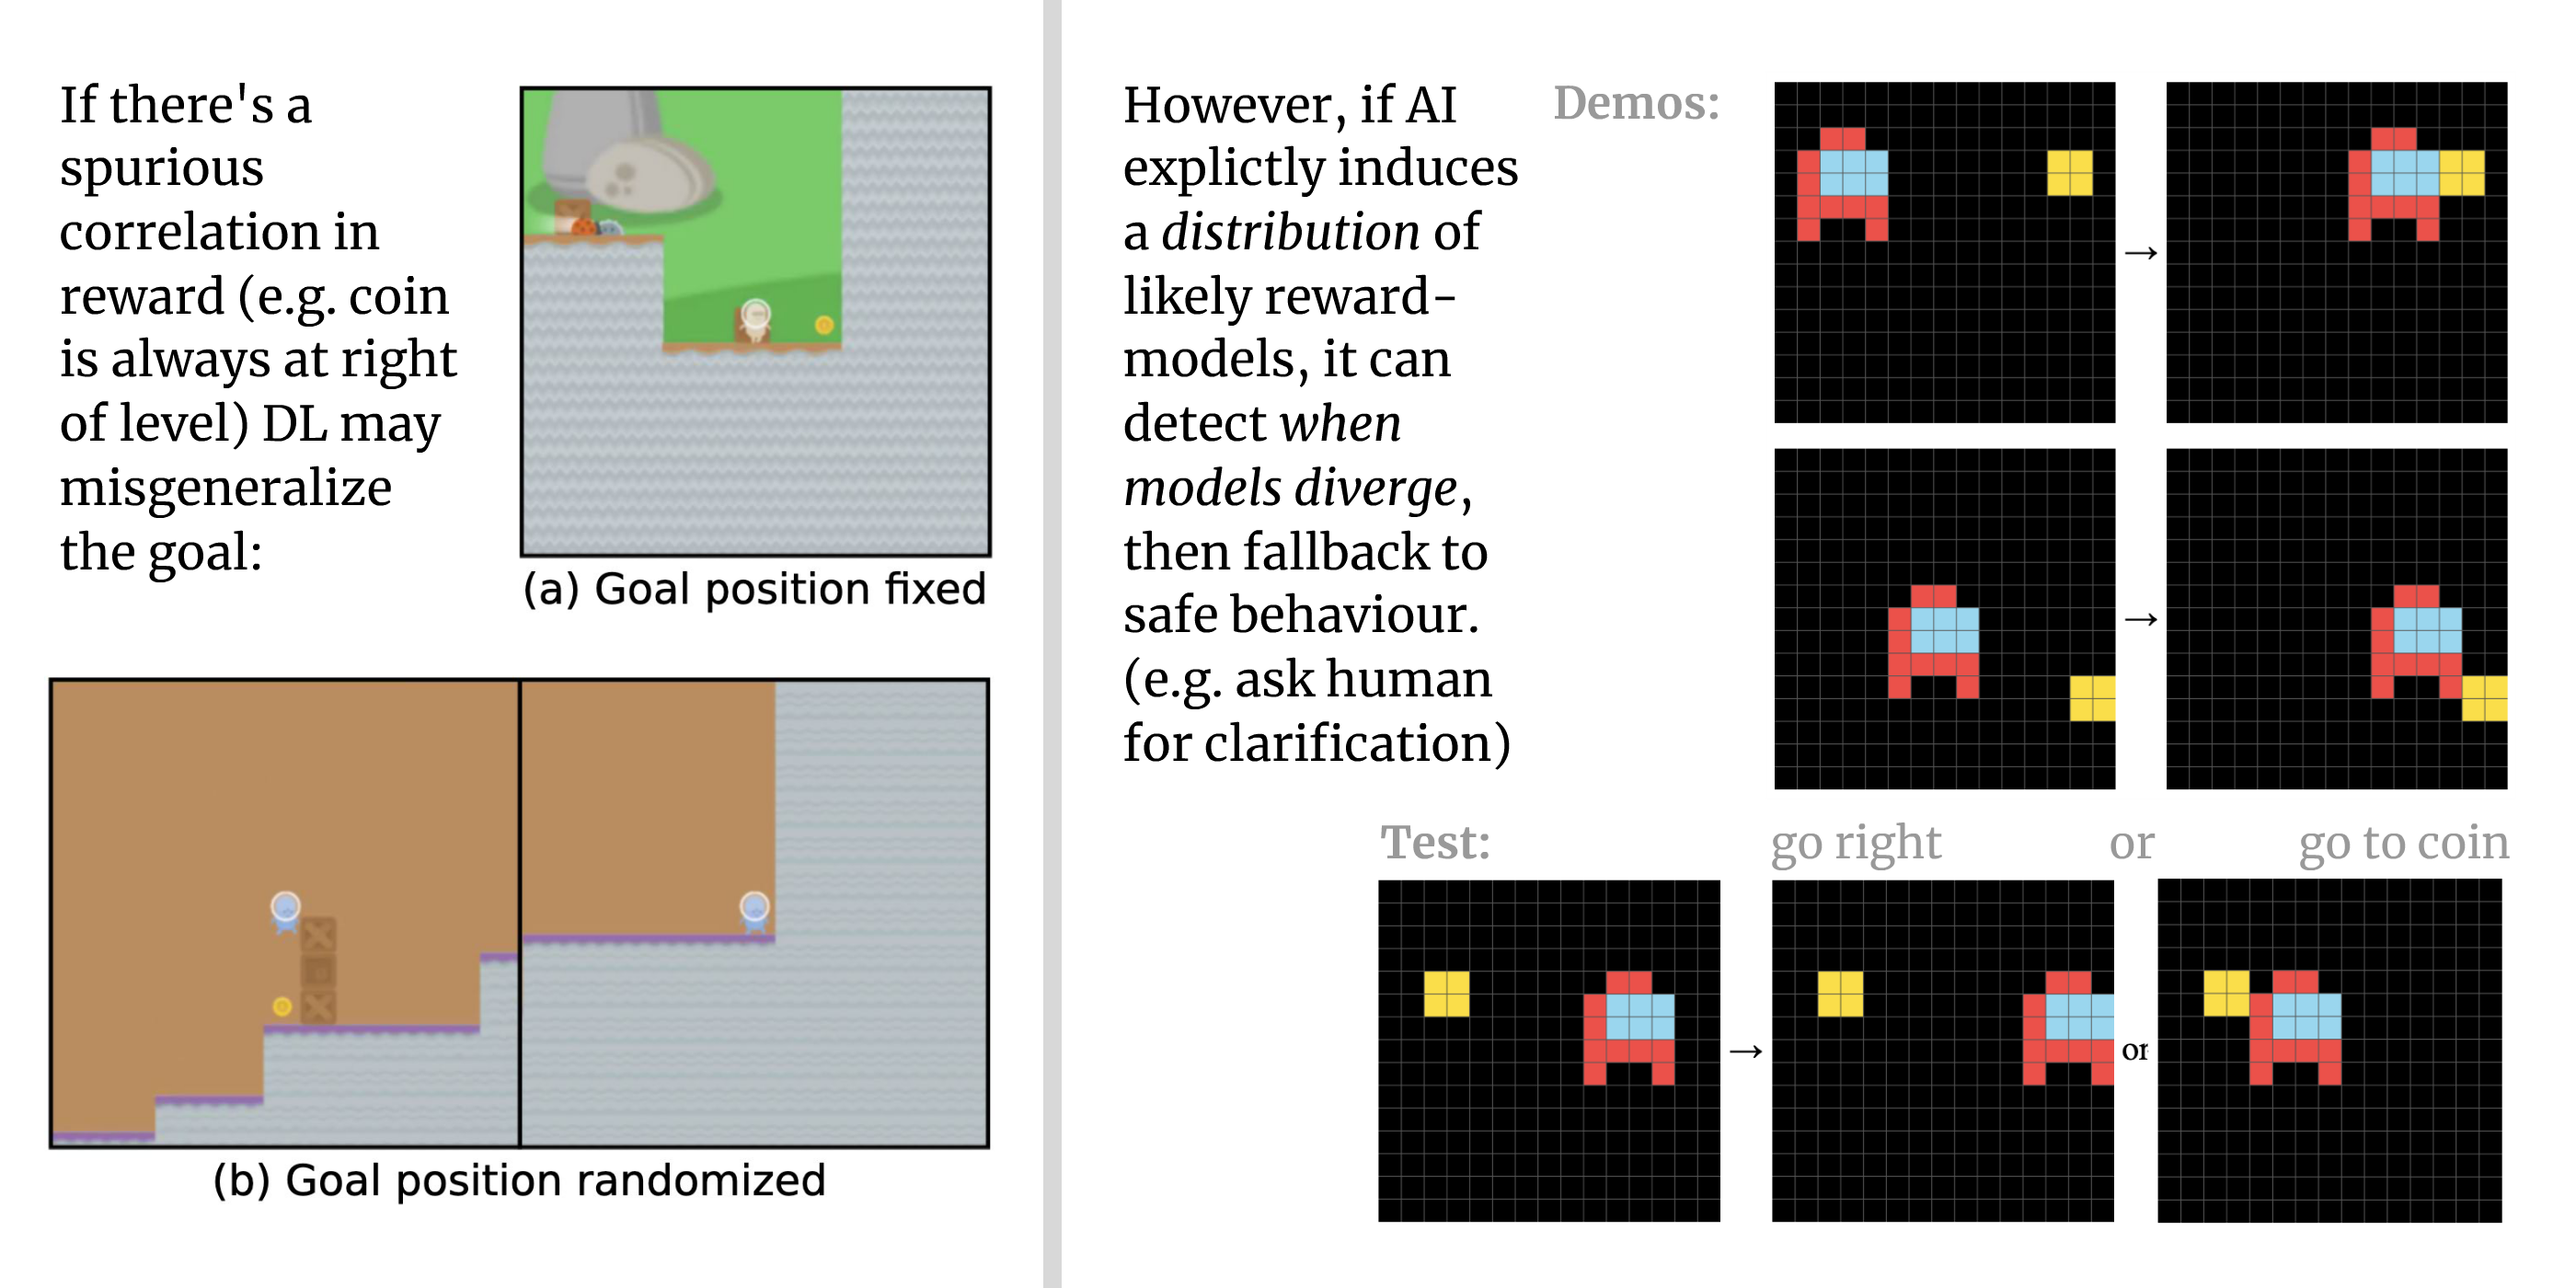
\includegraphics[width=\linewidth]{figures/across/coinrun.png}
    \caption{Left: Traditional DL misgeneralizes, by training on \textit{correlations}. Right: AlexNot circumvents this, by developing an ensemble of \textit{causal} models.}
    \label{fig:coinrun}
\end{figure*}

\textbf{For AI Safety:} If I'm planning a dinner party, it's \textit{not} dangerous if I don't know the guests' allergies: I can just ask them, clearly label all ingredients, avoid common allergens, etc. It's only dangerous if I don't know \textit{that I don't know} their allergies, and act recklessly. Likewise, it's \textit{not} dangerous if an AI doesn't know a human's values: it can just ask for clarification, give the human options, err on the side of caution. It's only dangerous if the AI \textit{does not know it does not know} what the human wants.

For a concrete example, let's look at the classic case study of ``inner misalignment'' \citep{risks_learned_optimization} or ``goal misgeneralization'' \citep{goal_misgeneralization} in the game CoinRun. (See \autoref{fig:coinrun}) In this experiment, they train an AI to get the coin that's always at the end of each level. However, the AI does \textit{not} learn the policy, ``go to the coin at the end of the level'', it learns a policy that \textit{is} simpler, compression-wise: \textit{``go to the end of the level''}. So on deployment levels where the coin is \textit{not} at the end, the AI will \textit{competently} keep going right, and ignore the coin. This is a toy example of an AI loss-of-control risk: an AI \textit{excellently} executing on a wrong goal.

But what if an AI not only formed an \textit{explicit} model of what the human wants, but \textit{a Bayesian distribution} of models? \autoref{fig:coinrun} shows a proof-of-concept of AlexNot solving the CoinRun goal-misgeneralization problem. AlexNot \textit{does} induce ``go right'' as a possible program, but it \textit{also} induces ``go to coin'' as well, since both fit the Demos equally well. And on the Test case where they diverge, it can correctly give both answers.

More generally: if an AI can induce \textit{multiple} models of what a human's goal is, it can detect OOD cases where these models diverge, then fall back to safe behaviour: stop \& ask for clarification, err on the side of caution \& reversible actions, etc.

This is related to the `indirect normativity' \citep{superintelligence,christiano_indirect_normativity} and `inverse reinforcement learning' \citep{russell_irl,inverse_rl} proposals: instead of trying to directly formalize what we value, get an AI to \textit{induce} models of our values, from what we say, do, and choose. (Inducing robust causal models from noisy sparse data is something any AGI worth calling ``AGI'' should be good at.) And crucially, induce \textit{a probability distribution} over those models, so when they diverge, the agent can default to safe behaviour.

\subsection{Summary, Limitations, Future Research}

In summary, Problem-Solving (and Problem-Finding!) is Search:

\begin{itemize}
    \item Open-ended innovation is search for paths in connected-idea space. The low-depth/high-width nature of this space explains the paradox of why genius seems obvious in hindsight.
    \item The human brain does search by having lots of parallel modules (System 1/subconscious) compete to have thoughts selected by a small bottleneck (System 2/consciousness) and broadcast back to all modules for further thinking, repeat. See: Global Workspace Theory (GWT).
    \item AlexNot imitates GWT with an execution-guided, island-model evolutionary search, guided by intelligent pattern-matching heuristics (``monkeys''), each one corresponding to a Core Knowledge Prior.
    \item AlexNot also does two helper searches, brute-forced over a small space: search for best Parser config, and search for best Bongard/Causality separator to propose ``all shapes with properties X,Y do Z''.
    \item Finally, AlexNot also generates not just one best solution, but a whole approximated Bayesian distribution of solutions, with out-of-model uncertainty. \textit{Knowing what you don't know} is a prerequisite for science, exploration, and safe, aligned AI.
\end{itemize}

Some limitations of our approach, and ideas for future research:

\begin{itemize}
    \item We \textit{only} searched for the best compressed world models to explain data (What ARC-AGI-1/2 tests). We did not try then \textit{using} these discovered world models, to search for \textit{actions} to solve problems. (What ARC-AGI-3 tests.) We did not try problem-\textit{finding}, the key to open-ended scientific breakthroughs. (What ARC-AGI-4 will test.)
    \item We generated an approximate Bayesian distribution of world models, but did not try searching for ``optimal experiment designs'' to efficiently \textit{distinguish} between plausible world models. (This would complete the loop in AI-amplified science: observe $\to$ hypothesize $\to$ \textit{experiment} $\to$ observe, repeat.)
    \item Even though we deliberately eschewed ML for the sake of research focus on symbolic reasoning, we're unsatisfied with how manually-tuned AlexNot's evolutionary search is: the search's hyper-parameters, doing scene-parsing separately from scene-transforming, etc. A future AI should be able to fluidly \& independently \textit{search for ways to improve its own search}. (In the later \hyperref[sec:limitations]{Future Research} section, we'll sketch a design for a DreamCoder+LLM+AlexNot neuro-symbolic hybrid, to address exactly this.)
\end{itemize}





%%%%%%%%%%%%%%%%%%%%%%%%%%%%%%%%%%%%%%%%%%%%%%%%%%%%%%%%%%%%%%%%%%%%%%%%%%%%%%%%%%%%%%
%%%%%%%%%%%%%%%%%%%%%%%%%%%%%%%%%%%%%%%%%%%%%%%%%%%%%%%%%%%%%%%%%%%%%%%%%%%%%%%%%%%%%%
% INTUITION is PATTERN-MATCHING
%%%%%%%%%%%%%%%%%%%%%%%%%%%%%%%%%%%%%%%%%%%%%%%%%%%%%%%%%%%%%%%%%%%%%%%%%%%%%%%%%%%%%%
%%%%%%%%%%%%%%%%%%%%%%%%%%%%%%%%%%%%%%%%%%%%%%%%%%%%%%%%%%%%%%%%%%%%%%%%%%%%%%%%%%%%%%

\section{Intuition is Pattern-Matching}\label{sec:pattern_matching}

\subsection{A Bag of Tricks}
\begin{quote}
\textit{``Cognition is recognition.''}

— Douglas Hofstadter (\citeyear{fluid_concepts})

\bigskip
\textit{``The situation has provided a cue; this cue has given the expert access to information stored in memory, and the information provides the answer. Intuition is nothing more and nothing less than recognition.''}

— Herbert Simon, as quoted in \citet{thinking_fast_and_slow}
\end{quote}
When you see ``$2^x - 7 = 9$, solve for $x$'', you don't re-derive the rules of algebra from scratch — you \textit{recognize} them, and automatically apply the if–then's. IF solving for x, THEN get x alone on one side. IF isolating x AND x is wrapped in some function, THEN apply the inverse.

Also note how \textit{physical} our metaphors for symbolic math are: ``balance the equation'', ``exponent hops down'', ``move to the other side''. (Whenever I see an inequality, I still visualize a tiny alligator trying to eat the bigger number.) Einstein himself cites visual \& muscular intuition \citep{hadamard_invention} for his theoretical insights, Terence Tao rolled around on the floor for his B\^{o}cher Prize-winning math paper \citep{tao_floor_anecdote}, mathematicians fruitfully use physical intuition to solve problems \citep{mathematical_mechanic}, and mathematical reasoning may ultimately be \textit{made up of} physical reasoning \citep{where_math_comes_from}.

Researchers like \citet{core_knowledge_priors} go further, and propose that, like how \textit{all} matter is composed of a few fundamental particles, \textit{all} human reasoning is fundamentally composed of pattern-matching on Core Knowledge Priors. Core Priors are the concepts that every normally-developing child has: folk physics, object permanence, a sense of `agentic' vs `non-agentic' things (e.g. animals vs rocks), and so on. There's a live debate on how much Core Priors' universality is due to common hardwiring (like the knee-jerk reflex) or due to common environment (we all grow up on planet Earth). Our paper is agnostic on the origin of Core Priors, but either way, they make a great `starter pack' for AlexNot's efficient induction of causal world models.

AlexNot's code-heuristics (``monkeys'') usually implement one Core Prior each. Mostly from  Spelke \& Kinzler's original list, but since their paper was never intended to be the final word, we added a few more. To avoid overfitting to ARC, we add a Core Prior \textit{only if} it's a concept most human toddlers would have, such as: patterns, ``visual focus'', and — most importantly — \textit{causality}.

A very brief summary of all Core Priors explicitly used in AlexNot code-editing monkeys:

\begin{figure*}[b]
    \centering
    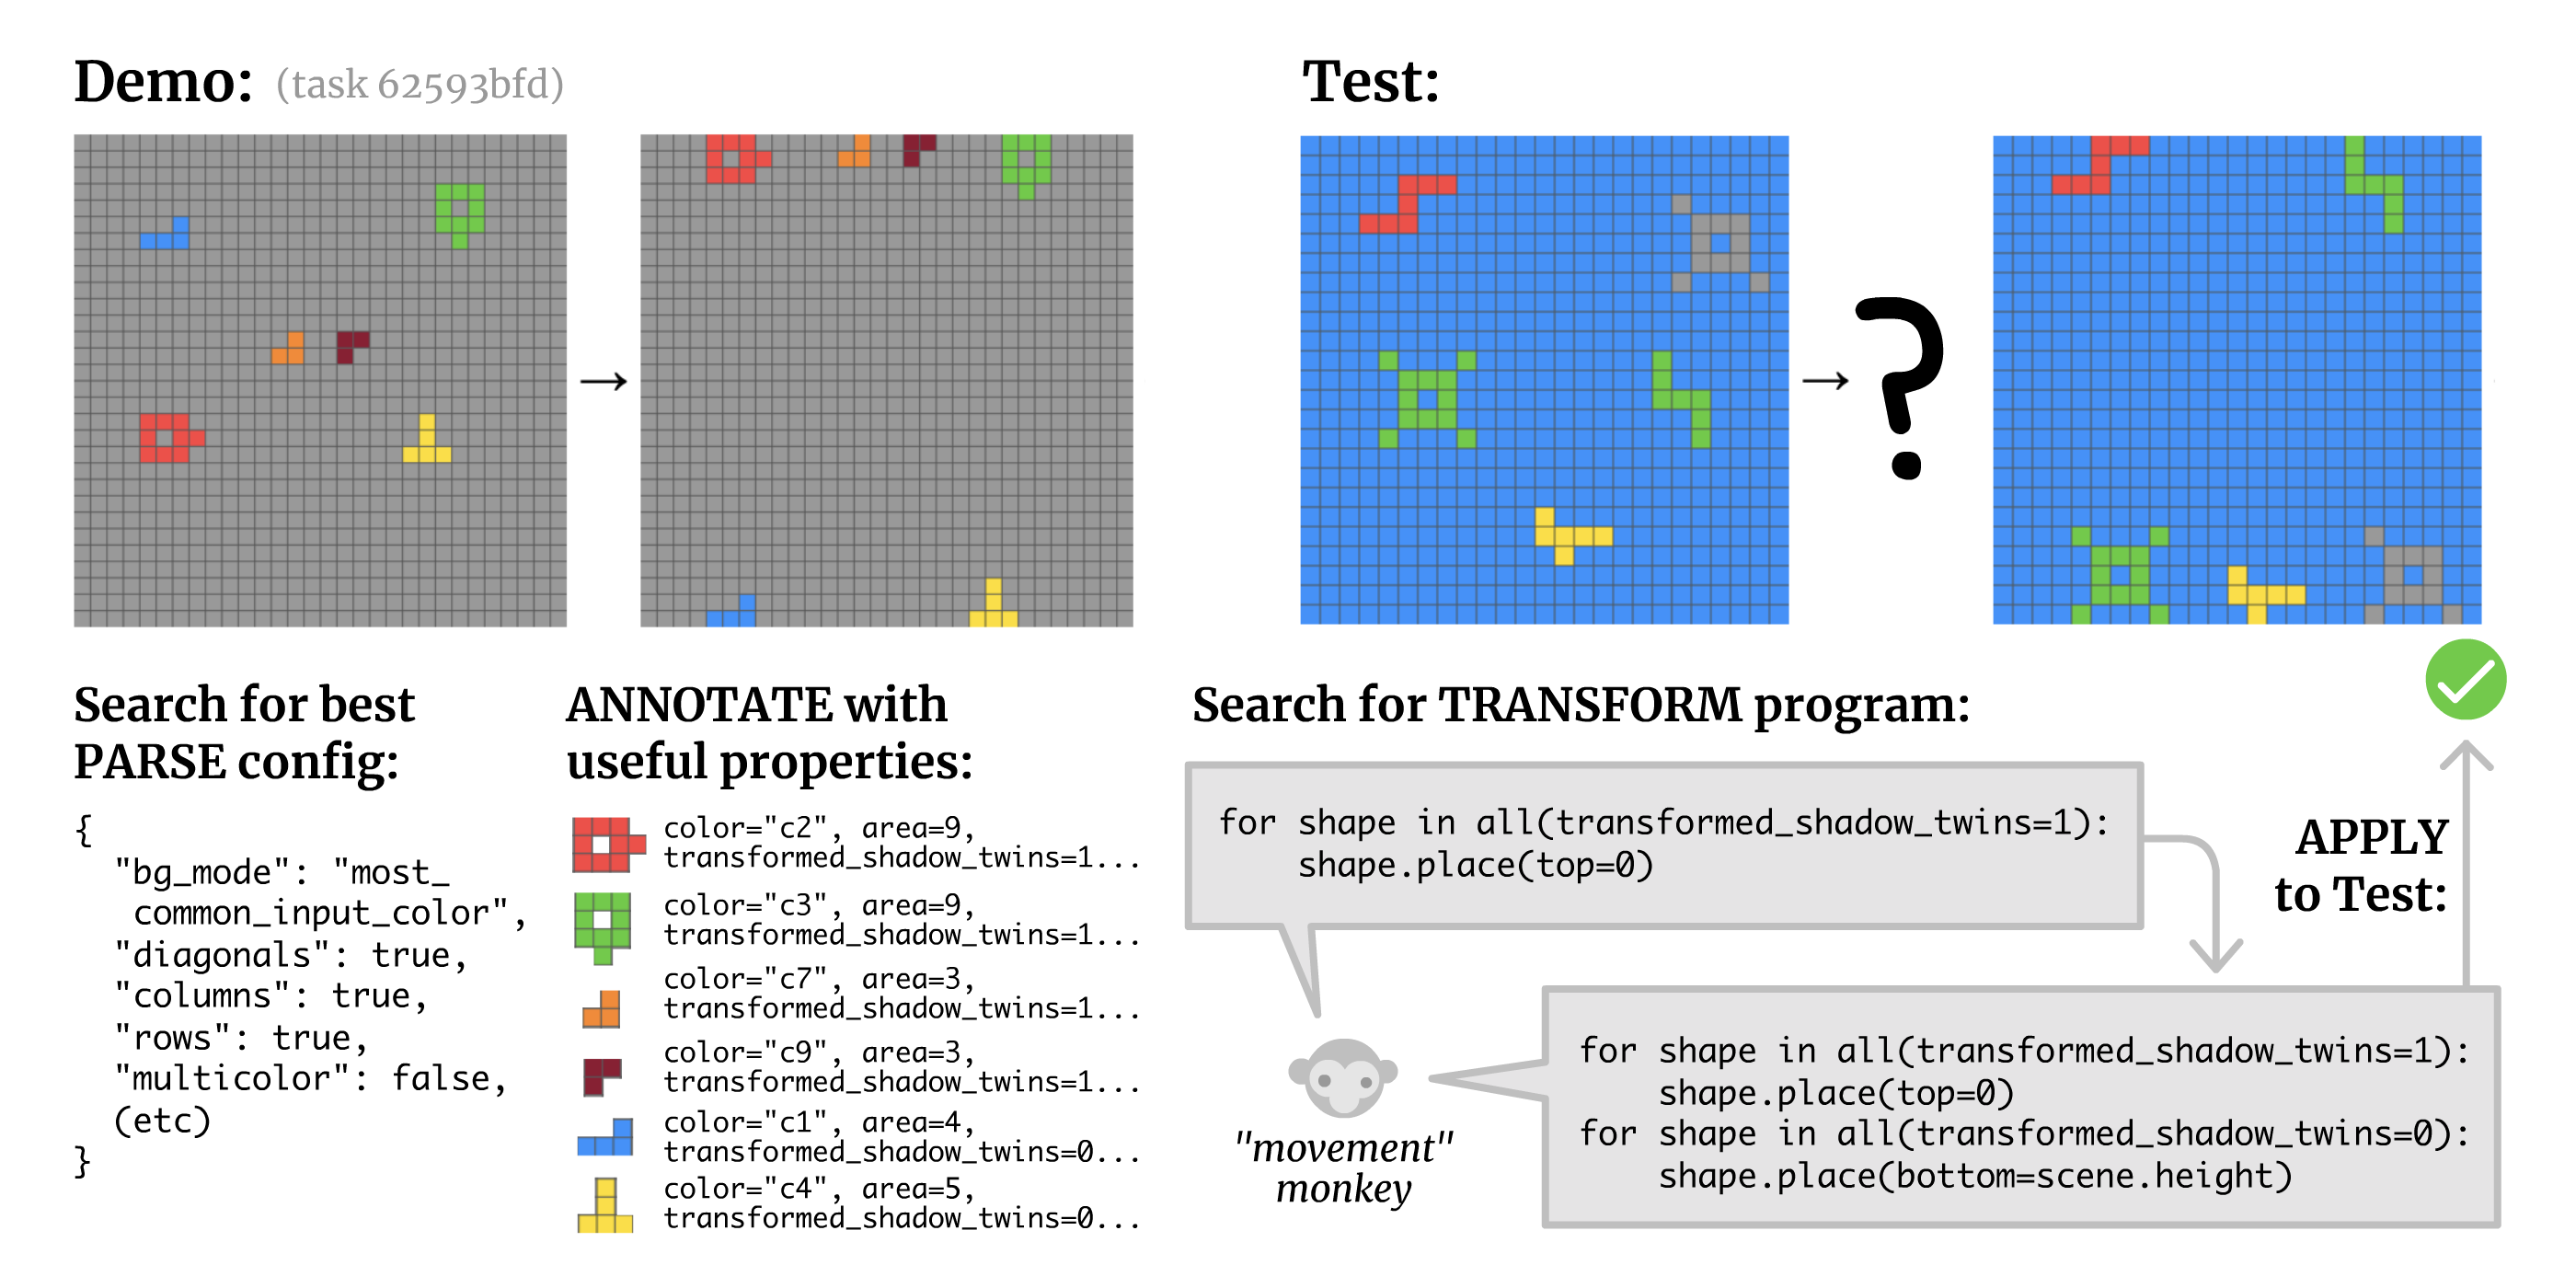
\includegraphics[width=\linewidth]{figures/across/twins.png}
    \caption{All stages of AlexNot, on an ARC-AGI-2 task.}
    \label{fig:twins_level}
\end{figure*}

\begin{itemize}
    \item Movement (2D): absolute placement, relative movement
    \item Movement (3D): moving `up' or `down' layers
    \item Geometry/Topology: area, holes, touching, proximity, shadow/silhouettes
    \item Transformations: rotations, flipping, symmetry
    \item Color: recoloring, filling holes
    \item Same vs Different
    \item Growth vs Shrink: shapes getting outlines / insets
    \item Create / Copy / Destroy
    \item Counting, Rank/Order
    \item Patterns
    \item Folk Physics: gravity, attraction, light beams
    \item Agentic Actions: fitting shapes into gaps, matching shapes onto patterns, connecting, sorting
    \item Visual Focus: crop the output scene to highlight specific shape(s)
    \item Coincidence \& Causality: \textit{why} are these two things connected?
\end{itemize}

(A few glaring omissions: scaling shapes, fractals, basic arithmetic. See the \hyperref[sec:pattern_matching_limitations]{Limitations} section below.)

The only code-editing monkeys that do \textit{not} use a human-universal Core Prior, but are still general/not specific to ARC, exist for the sake of compression \& exploring program-space: randomly deleting code, randomly re-arranging code-blocks, etc.

For more details on every monkey, check \url{https://github.com/ncase/alexnot/blob/main/docs/MONKEYS.md}

\subsection{Anatomy of a Monkey}

Let's see the monkey responsible for the ``movement'' Core Prior in action. (\autoref{fig:twins_level}) In the process, it interacts with 4 more Core Priors: same-different, transformations, topology, and causality.

First, our solver parses the pixel grids into a scene with shapes, and annotates them with lots of helpful properties. In this case, the annotation step notices that multiple shapes have \textit{the same shadow as another shape on the scene}, up to rotations/flips.

Next, in Round 0 of ``search for transform'', the Movement Monkey notices some shapes go up. It calls the Bongard/Causality helper search, and finds what property they all have in common, that the others don't. Answer: all the shapes that go up, and only them, are annotated \texttt{transformed\_shadow\_twins=1}! The monkey proposes this program, it wins, and in Round 1, it cleans up the remainder: all shapes annotated \texttt{transformed\_shadow\_twins=0} go \textit{down}. After this, all pixels are explained, and the search can't find a shorter program, so the evolutionary search ends early, and we get our solution!

(How's the monkey know \textit{that's} the property that matters, and not some other coincidental property? Answer: it doesn't! Each Monkey can propose up to 100s of programs; because this all runs on raw Python and numpy, it's easy to generate and test 1,000s of programs in a few seconds.)

\subsection{Pure-Symbolic Heuristics Actually Have Quite A Lot Going For Them?}

When we first started this research project — challenging ourselves to see how far we could get \textit{without} ML or deep learning — we expected to find that pattern-matching would be the \textit{worst} match for pure-symbolic code, and \textit{obviously} a good Neuro-Symbolic system should swap them all out for neural pattern-matchers.

And outside of ARC's gridworld tasks, yes, obviously neural networks have been far more successful at real-world perception than pure code. But there's 3 advantages of pure-code pattern-matchers, that we didn't appreciate before starting this project:

\begin{itemize}
    \item \textbf{Speed!} Each monkey can generate 100s of proposals \textit{in milliseconds}. Claude Haiku wouldn't even finish a single line of code before then.
    \item \textbf{Can do \textit{explicit} search.} Neural networks \textit{do} perform search, implicitly: a multi-label classifier can be thought of as an ensemble of sub-networks, competing via softmax at the end. But a neural network would struggle to do what the above Movement Monkey did: explicitly search over \textit{exact} properties, like ``how many shapes share the same silhouette, up to rotations/flips?'' This is crucial for exact causal inference.
    \item \textbf{Can provide more useful variance.} Conventionally-trained neural networks tend towards mode collapse, and the naïve way of increasing variance (turn up the temperature) makes LMs produce ungrammatical garbage. But evolutionary search is antifragile \citep{taleb_antifragility_math}: it \textit{benefits} from higher variance. With symbolic code, it's easier to produce high-variance guesses, that are \textit{all} still grammatically correct and semantically meaningful. (\citet{mixture_of_concepts} tests a `Mixture of Concepts' approach in Mini-ARC, to get LLMs to generate more useful variance, by directly prompting them to think about different concepts first. Still, LLMs are slow compared to pure-code.)
\end{itemize}

\begin{figure}
    \centering
    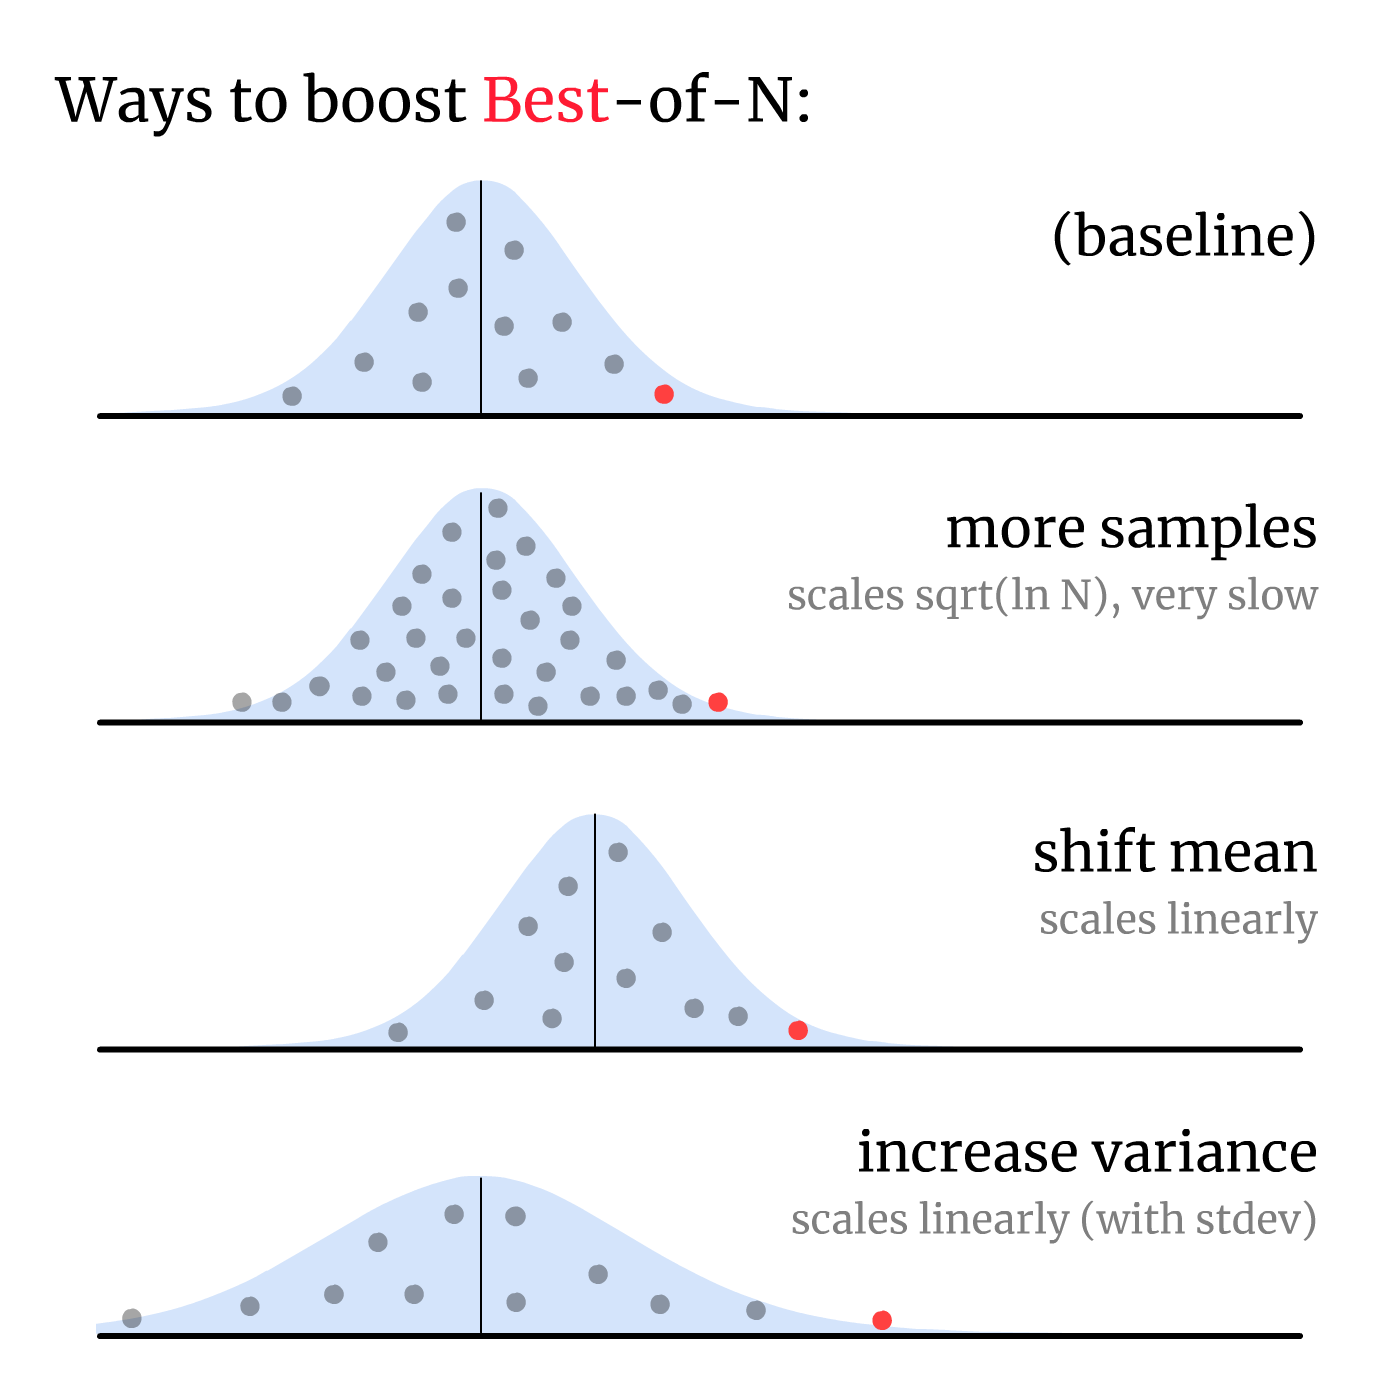
\includegraphics[width=\linewidth]{figures/mini/antifragile.png}
    \caption{Ways to boost Best-of-N performance, from (typical) least-to-most effective.}
    \label{fig:antifragile}
\end{figure}

To elaborate on ``antifragility'': even if a pure-code heuristic is on average \textit{much worse} than its pure-neural counterpart, it may \textit{still} be better to use in an evolutionary search. Why? Because an evolutionary search picks the best-of-N every round, and best-of-N can be boosted in three main ways: increase mean, increase variance, increase samples. (See \autoref{fig:antifragile}) Of the three, \textit{increasing variance has highest bang-for-buck}. Increasing average performance is hard, increasing samples scales \textit{sub}-logarithmically (see: diminishing returns on OpenAI swarm size \citep{ord_swarm_scaling}), but adding grammatically-correct random exploration over models is cheap with symbolic code.

So, while neural networks will still be needed for real-world perception \& action, it seems like an AI's heuristics shouldn't be \textit{pure}-neural. For the sake of speed, variance, and explicit search, even the pattern-matchers could be Neuro-Symbolic hybrids.

\subsection{Summary, Limitations, Future Research}\label{sec:pattern_matching_limitations}

In summary, efficient search needs `intuition': a bag of tricks, a starter pack of pattern-matchers, most likely based off the human-universal Core Knowledge Priors.

\begin{itemize}
    \item One of the most valuable Core Priors we found, not explicitly listed in \citet{core_knowledge_priors}, was \textit{causality.} It was crucial for our code-generator heuristics to use a shared utility function (The Bongard Function) to do exact causal inference on why which shapes did what.
    \item Contrary to our expectations, there's some clear wins for symbolic over neural even in the heuristics: more useful variance, explicit search, speed. Future AI designers may want to consider making even the \textit{heuristics} Neuro-Symbolic hybrids, too.
\end{itemize}

Limitations of the theory \& our implementation, and ideas for future research:

\begin{itemize}
    \item Nobody knows what the true list of all human-universal Core Priors is, and we didn't even implement all the ones we \textit{did} know about.
    \item Even if we had an objective list of all human Core Priors, it's not clear if AI should use \textit{fewer or more} priors than that. Analogy: planes don't fly like birds, and they \textit{shouldn't}; planes have it harder than birds on some dimensions (must carry 100+ humans comfortably) and easier than birds on others (don't need to forage for their own fuel). Likewise, maybe we should use fewer Core Priors for AI because data is abundant; or maybe we should use \textit{more} Core Priors, because unlike humans' messy translation from DNA $\to$ proteins $\to$ neuron architecture $\to$ Core Prior, in software, you can just code things.
    \item By design, ARC-AGI requires \textit{only} the Core Knowledge Priors, and no higher-level pattern matching, like ``IF solving for x, THEN isolate x''. Writing \textit{every} pattern-matcher manually would be \textsc{The Ghost of Cyc} haunting us once more. But this is where LLMs can be the ``transition fuel''! Nowadays, even small LMs are decent at coding: we could ask LLMs to take the successful patterns in their own Chain of Thought, and convert those into pure-code heuristics, or hybrid heuristics like ``normal code that queries simple neural classifiers at key moments''. (Again, see Future Research for a fuller design sketch of a DreamCoder+LLM+AlexNot system.)
\end{itemize}




%%%%%%%%%%%%%%%%%%%%%%%%%%%%%%%%%%%%%%%%%%%%%%%%%%%%%%%%%%%%%%%%%%%%%%%%%%%%%%%%%%%%%%
%%%%%%%%%%%%%%%%%%%%%%%%%%%%%%%%%%%%%%%%%%%%%%%%%%%%%%%%%%%%%%%%%%%%%%%%%%%%%%%%%%%%%%
% RESULTS & EXPERIMENTS
%%%%%%%%%%%%%%%%%%%%%%%%%%%%%%%%%%%%%%%%%%%%%%%%%%%%%%%%%%%%%%%%%%%%%%%%%%%%%%%%%%%%%%
%%%%%%%%%%%%%%%%%%%%%%%%%%%%%%%%%%%%%%%%%%%%%%%%%%%%%%%%%%%%%%%%%%%%%%%%%%%%%%%%%%%%%%

\section{Results \& Experiments}\label{sec:results}

\texttt{[30+ pages later...]}

\textit{Now} let's talk results. In this section, we'll show you:

\begin{itemize}
    \item AlexNot's main results on ARC-AGI-1/2, alone \& ensembled with NVARC (2025)
\item Does AlexNot ``know when it doesn't know''?
\item Ablation/variant experiments, and what they mean for the 3 Cognitive Science principles
\item A cherry-picked anecdote of AlexNot doing ``open-ended innovation'', re-inventing a mechanical-physical sorting algorithm
\item And finally, what we're most excited for: we present \textsc{AlexNot-ODE}, a minimalist variant of AlexNot, which can induce \textit{real-world} differential equations — in physics, life sciences, and business — from noisy, sparse data. This is to show off the flexibility \& generality of AlexNot's modular architecture, and show that its general design principles \textit{could} scale to real-world Scientist AI.
\end{itemize}

\subsection{Main Results}\label{sec:main_results}

\textbf{Absolute scores:}

As already reported in Section~\ref{sec:what_we_made}, the pure-symbolic AlexNot alone achieved the following scores on these ARC and ARC-like datasets: (re-runs may vary by $\pm3$\% due to the random nature of evolutionary search.)

\begin{itemize}
    \item \textbf{40.40\%} on Concept-ARC \citep{concept_arc}
    \item \textbf{32.20\%} on Mini-ARC \citep{mini_arc}
    \item \textbf{17.63\%} on ARC-AGI-1 Public Eval
    \item \textbf{13.33\%} on ARC-AGI-2 Public Eval
\end{itemize}

Again, at a mere cost of \textit{30 CPU-seconds per task}. That's \$0.000035 per task, over five thousand times cheaper than the already-highly-constrained winners from last year's contest (\$0.20/task). (See \autoref{fig:alexnot_scores_pareto} from Section~\ref{sec:what_we_made})

\textbf{Relative score drop from ARC-AGI-1 to -2:}

\begin{figure*}[t]
    \centering
    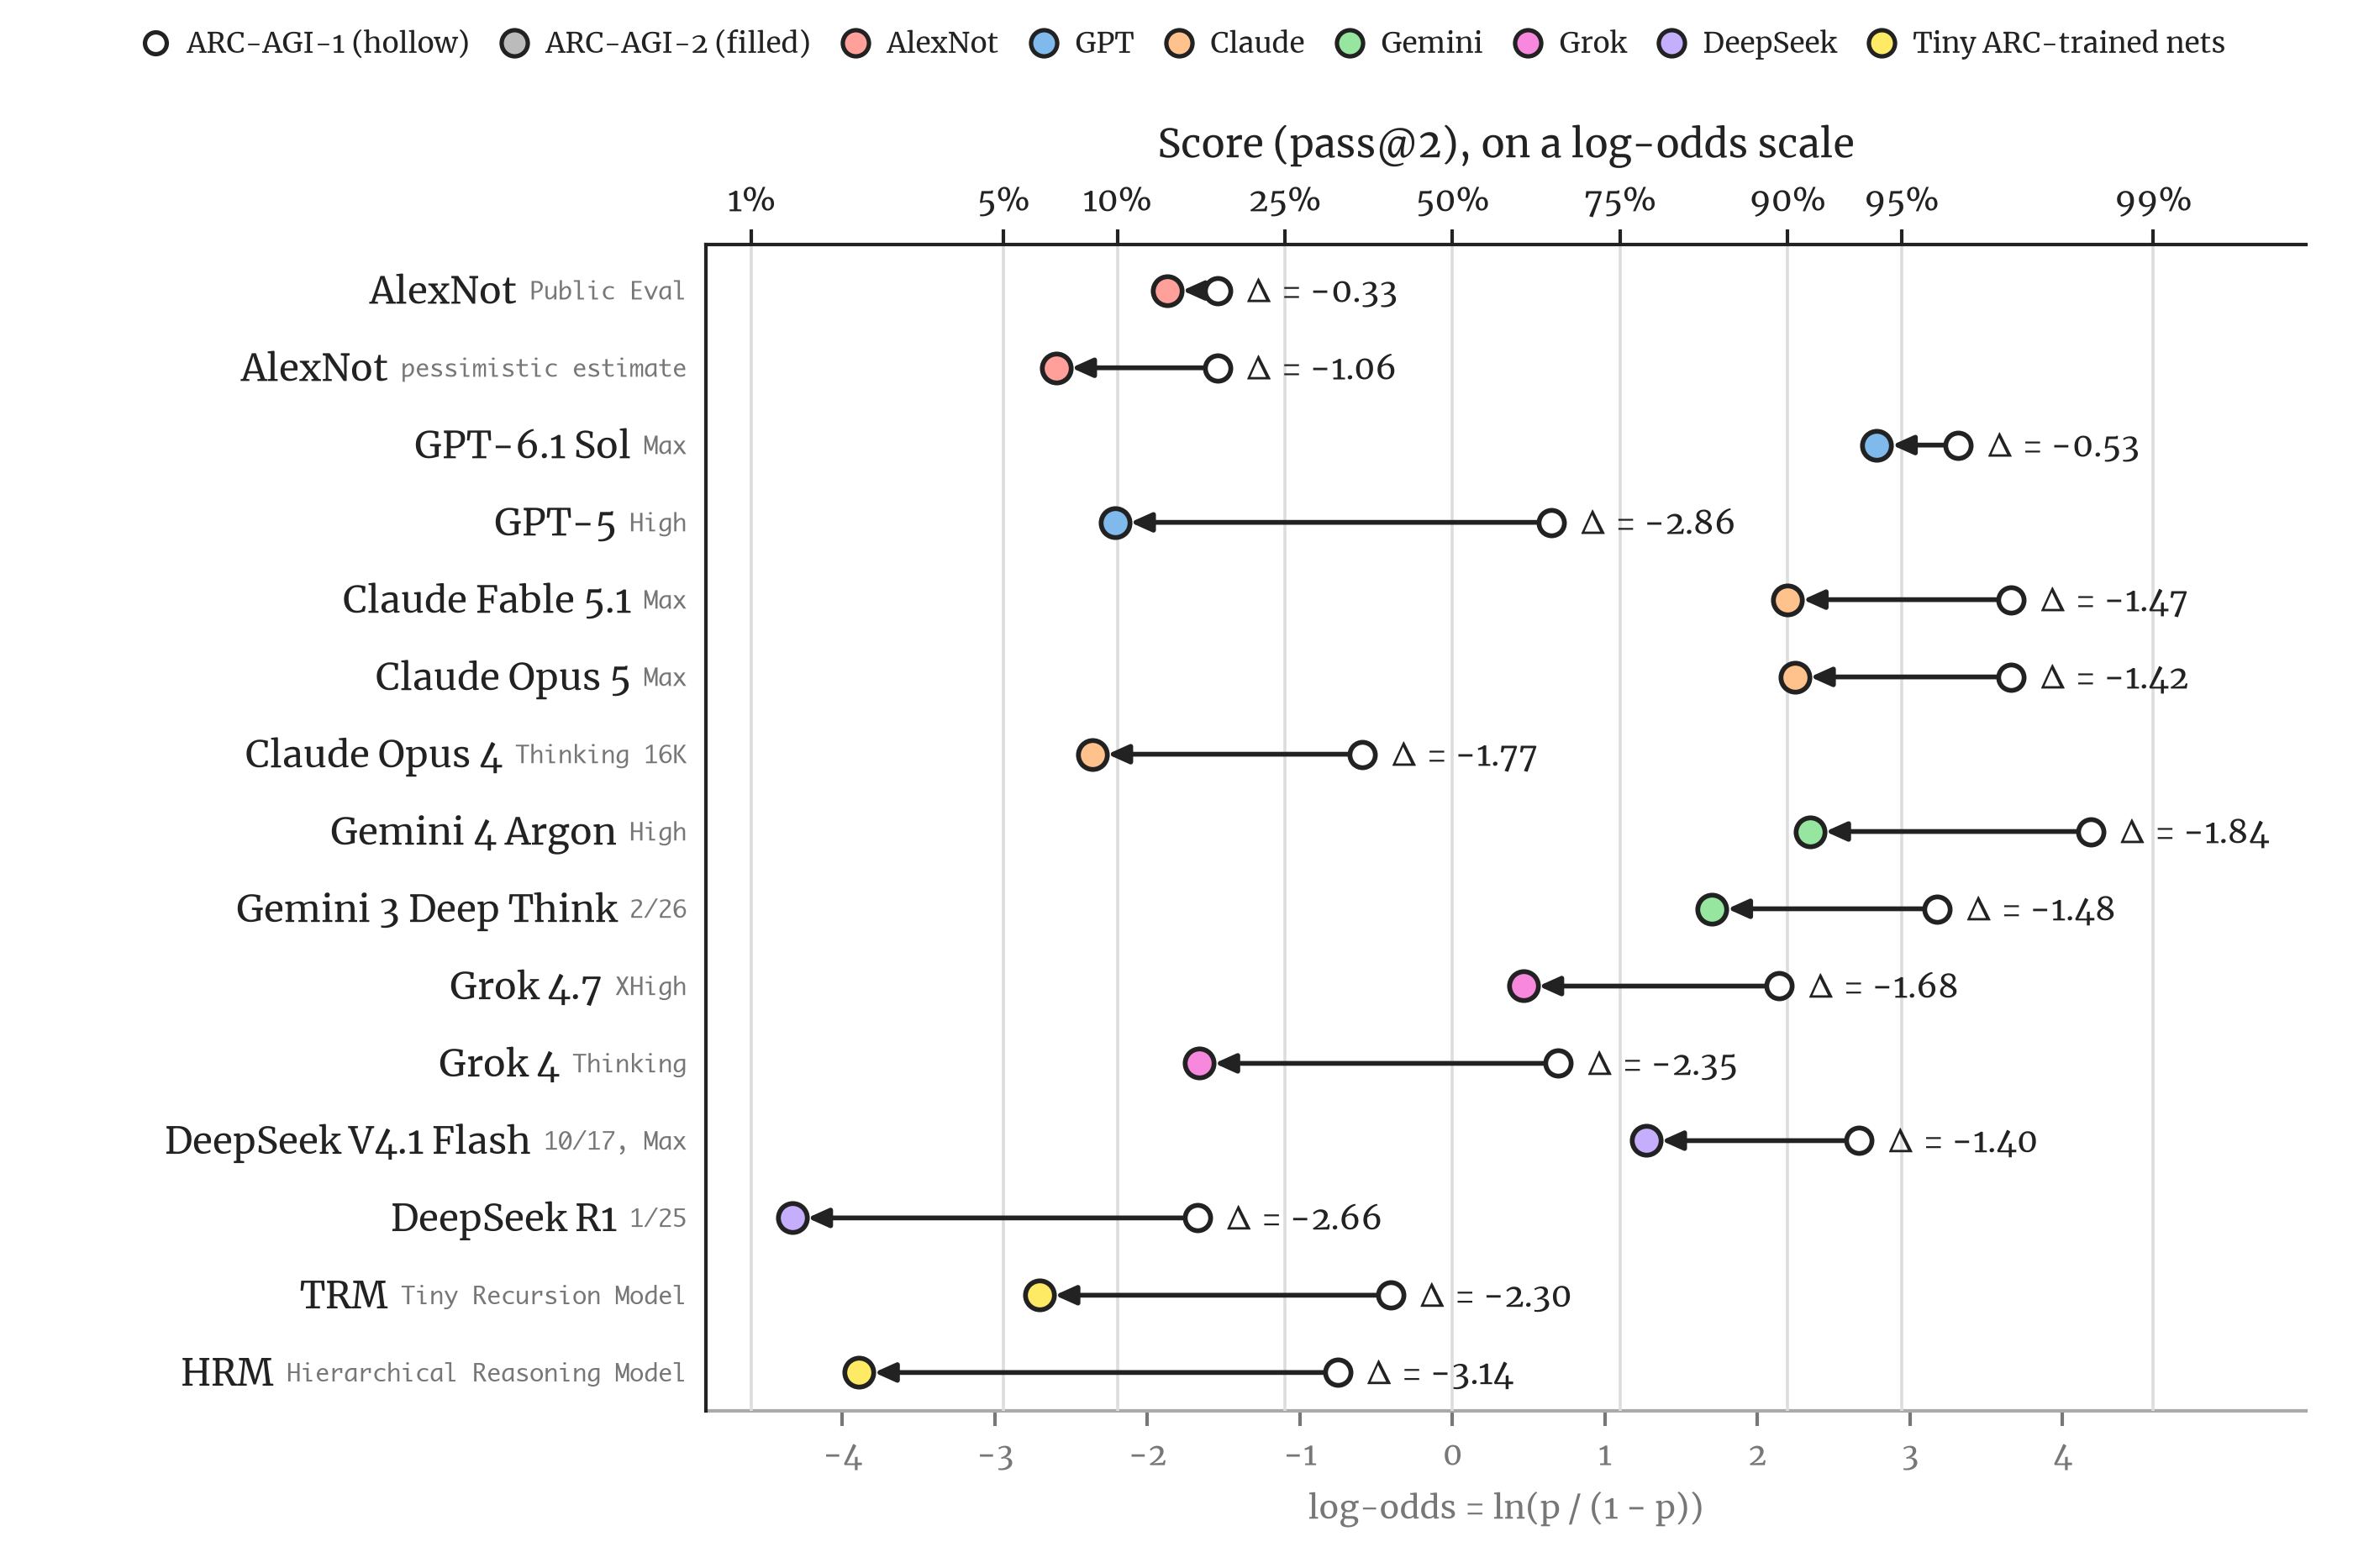
\includegraphics[width=\linewidth]{figures/dataviz/dumbbell.png}
    \caption{Log-odds performance drops from ARC-AGI-1 $\to$ -2, for AlexNot, the major LLMs, and TRM/HRM.}
    \label{fig:log_odds}
\end{figure*}

Compared to other neural solutions' absolute score, AlexNot sucks. But AlexNot's \textit{relative} drop in performance is better than \textit{almost every other major LLM and neural solution}, even if we use the pessimistic estimate for AlexNot's true Eval performance. (6.92\%, calculation a few paragraphs down.)

See \autoref{fig:log_odds}, for a log-odds plot of AlexNot, the major versions of the major frontier LLMs, and two tiny models, HRM \citep{hierarchical_reasoning_model} \& TRM \citep{tiny_recursion_model}. (We use log-odds because raw \% score compresses the ends too much, i.e. a 99\% $\to$ 95\% performance drop doesn't look too bad, but it's a fivefold increase in error.) On a log-odds scale, AlexNot's ARC-AGI-1$\to$2 score drop is only $-0.33$, better than everyone else. Using the more pessimistic estimate for AlexNot's true ARC-AGI-2 performance, it's $-1.06$, still better than everyone except GPT-6.1 Sol Max.

This is exactly what theory predicts: Neural excels at \textit{breadth}, but Symbolic excels at \textit{depth}. This is evidence for how symbolic-first approaches scale \textit{better} with more complex tasks.

\textbf{Why AlexNot fails when it does:}

For exactly the reason you'd expect — it doesn't have a necessary Core Prior. (Our DSL doesn't even have if-then statements, and can't detect shapes being scaled up/down, for instance.) Again, coding up these Core Priors — even with Claude Code assistance — was incredibly labour-intensive, hence why AlexNot has such little \textit{breadth}.

\textbf{Our contest submission: AlexNot + NVARC (2025) ensemble}


\begin{figure}[h]
    \centering
    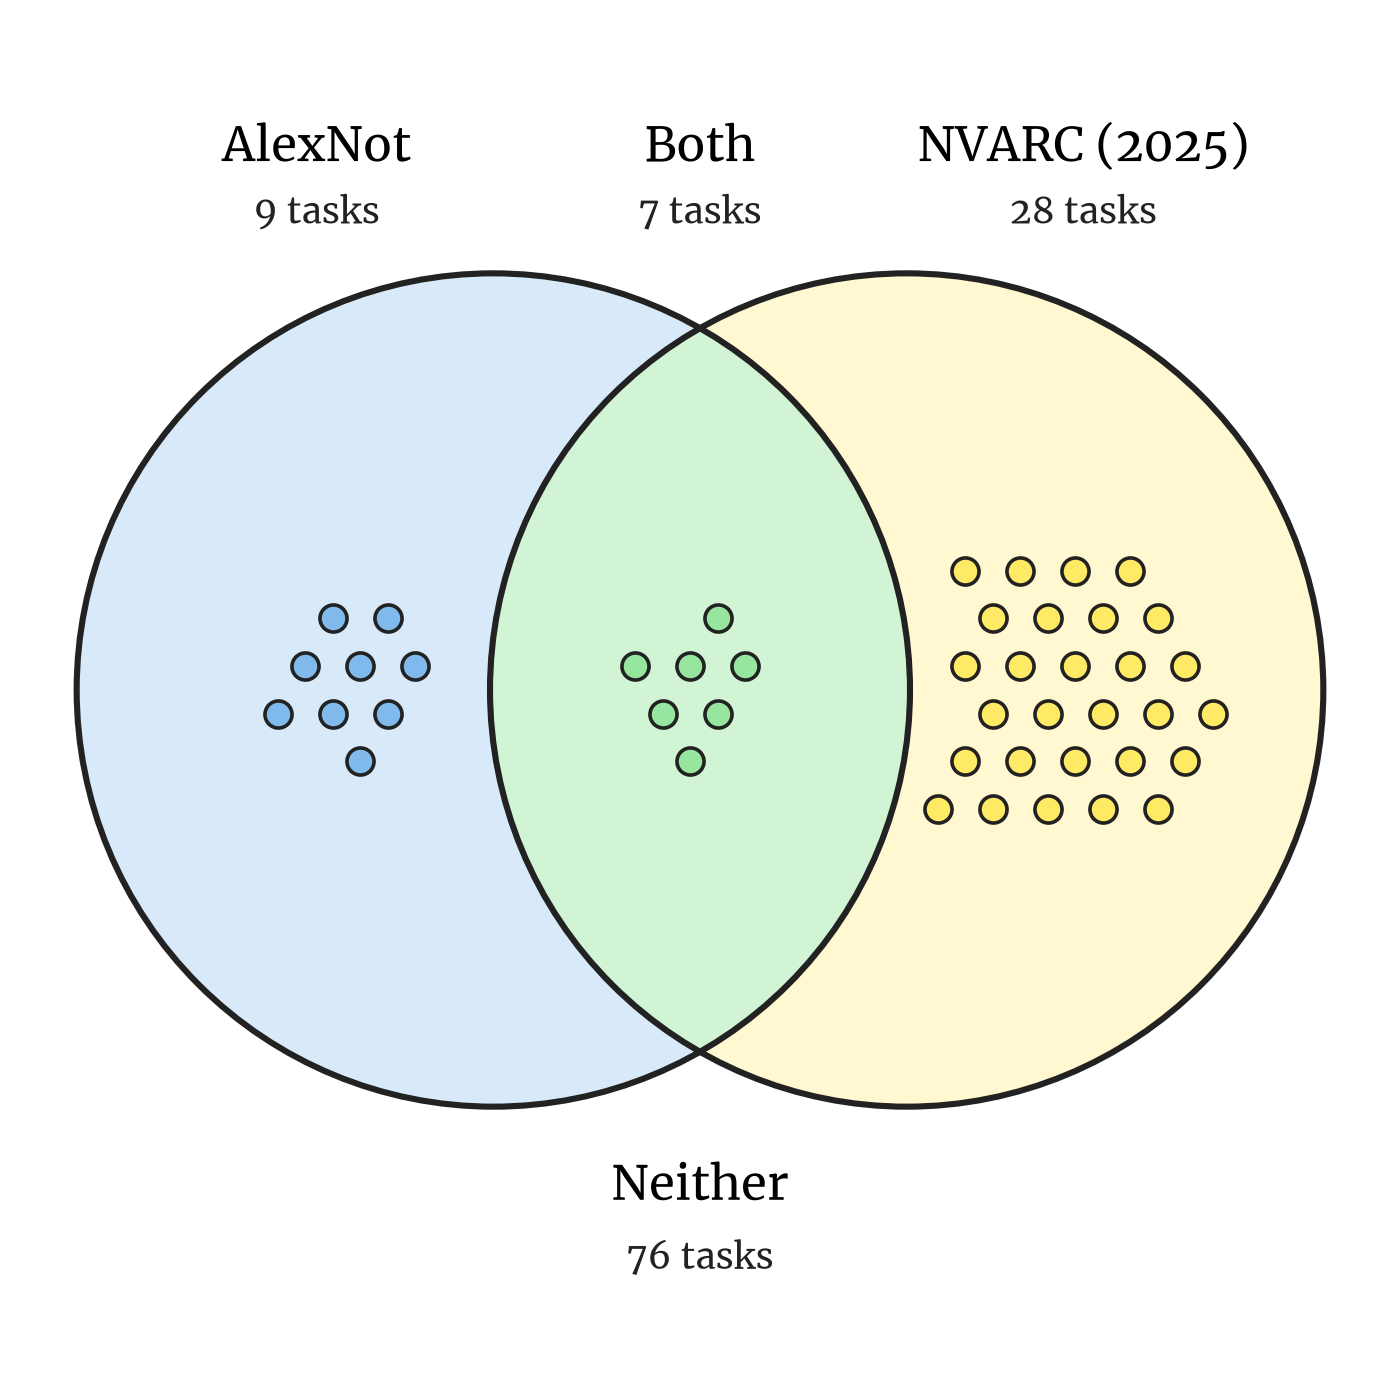
\includegraphics[width=\linewidth]{figures/dataviz/venn.png}
    \caption{Venn diagram of what ARC-AGI-2 Public Eval tasks AlexNot vs NVARC (2025) could \textit{fully} solve. For the sake of clarity, we only count a task as solved if it was pass@2 correct on all task Test inputs, no partial credit.}
    \label{fig:venn}
\end{figure}

But since AlexNot could blast through all 240 Semi-Private/Private Eval puzzles on Kaggle contest hardware in \textit{under 5 minutes}, out of a full 12 hour (720 minute) time budget, we ensembled it with last year's \#1 winner, NVARC \citep{nvarc_2025}, an optimization of ARChitects \citep{architects_2024} trained on 3.2M synthetic examples.\footnote{We made only a few small tweaks to NVARC (2025), none of which helped improve its performance above seed noise, which was $\pm3$\%. In fact, the ``biggest'' fix we made \textit{was} a seed problem: the original code forgot to change its random seed per task. This is another reason why it's hard to directly compare our scores: seed noise alone is $\pm3$\%.} Together, our ensemble got \textbf{31.53\%} on the public Kaggle leaderboard. For comparison, NVARC scored 27.64\% on the public LB last year \citep{2025_LB}. Assuming the same tasks were re-used, that's a +3.89\% improvement. Small, but beyond seed noise, showing how neural + symbolic is better than either alone. (\textit{NOTE: This is a very noisy estimate, but given the lack of clean comparison, it'll have to do.})

We can get a Venn diagram on the ARC-AGI-2 \textit{Public} Eval, to see what tasks pure-symbolic AlexNot vs pure-neural NVARC gets. See \autoref{fig:venn}. Our results conceptually replicate \citet{induction_transduction}, which found that on ARC-AGI, inductive approaches (figure out the actual rule) and transductive approaches (directly predict output) complement each other: they overlap, but not fully.

\textbf{Did we overfit?}

This Venn diagram also lets us estimate what AlexNot-alone \textit{would} have gotten on the public Kaggle leaderboard/Semi-Private Eval!\footnote{Due to the 1-submission-a-day limit, we didn't want to waste it, and only submitted the ensemble. We thought Late Submissions would be open, and we could submit AlexNot-only to get a clean comparison score, but Late Submissions were closed when we tried on Nov 8.} This will let us identify \& report overfit. On the ARC-AGI-2 \textit{Public} Eval, AlexNot solved 16 tasks fully, 9 of which were AlexNot's addons above NVARC. So, the full-to-addon ratio is around 16/9, or $\sim$1.778. As estimated above, on the \textit{Semi-Private} Eval (Kaggle leaderboard), AlexNot added a +3.89\% improvement. So, assuming the score-to-addon ratio is about the same, AlexNot-alone \textit{would} have scored a 3.89\% $\times$ 1.778 $=$ 6.92\% on the Kaggle leaderboard. (\textit{Again: this is a HORRIBLY noisy estimate}, but in the absence of a clean comparison, it's the best we can do. Also, if you're from ARC Foundation and reading this, you can just test AlexNot on the Private Eval in a couple minutes on a laptop. Hooray CPU-only.)

6.92\% \textit{is} a lower score than 13.33\%, suggestive of overfit. But: a) it's not statistically significant at p<0.05 (p=0.13\footnote{Fisher's exact test: p=0.13 two-sided, p=0.07 one-sided. This is Public Eval 16/120 vs. Semi-Private 8/120 (6.92\% rounded down, which favours finding overfit). Note 6.92\% is itself a noisy estimate built on $\pm3$\% seed noise, so the true p-value is likely even higher/less significant.}), since each dataset is N=120, and at N=120, a 10\%-accurate solver would have a huge observed 95\% CI of [5.3\%, 16.8\%]. Also, b) 6.92\% is still on par with last year's Top 5 \textit{Private} scores \citep{arc_prize_2025_results}, and still 5,000$\times$ cheaper.

Still, \textit{if} we had overfit to ARC-AGI-2 Public Eval, how? We \textit{only} ever implemented the Core Knowledge Priors. And the pure-symbolic code is transparent and open-source, you (or your favourite coding agent) can check, there's nothing hidden up our sleeve. But as mentioned earlier, while we \textit{only} implemented Core Priors, we ran out of time to implement \textit{all} of them. So, likely, we disproportionally implemented the ones whose \textit{combination} we knew was in the Public Eval. (We manually played \textit{all} ARC-AGI-1/2 Train/Eval tasks. They were fun! Mostly.) ARC-AGI-2 tasks, compared to ARC-AGI-1, used \textit{lots more} Core Priors composed together. For example, the ``twins up, else down'' puzzle in \autoref{fig:twins_level} used \textit{five} Core Priors: movement, same-different, transformation, topology, causality. So, \textit{if} AlexNot was overfit to the Public Eval — and again, the p-value was suggestive but not statistically significant at p<0.05 — it'd be due to the \textit{combinations} of Core Priors, not the Core Priors themselves. The heuristics remained fully general. 

\subsection{Does AlexNot know when it doesn't know?}

We have good news \& bad news.

\begin{figure}
    \centering
    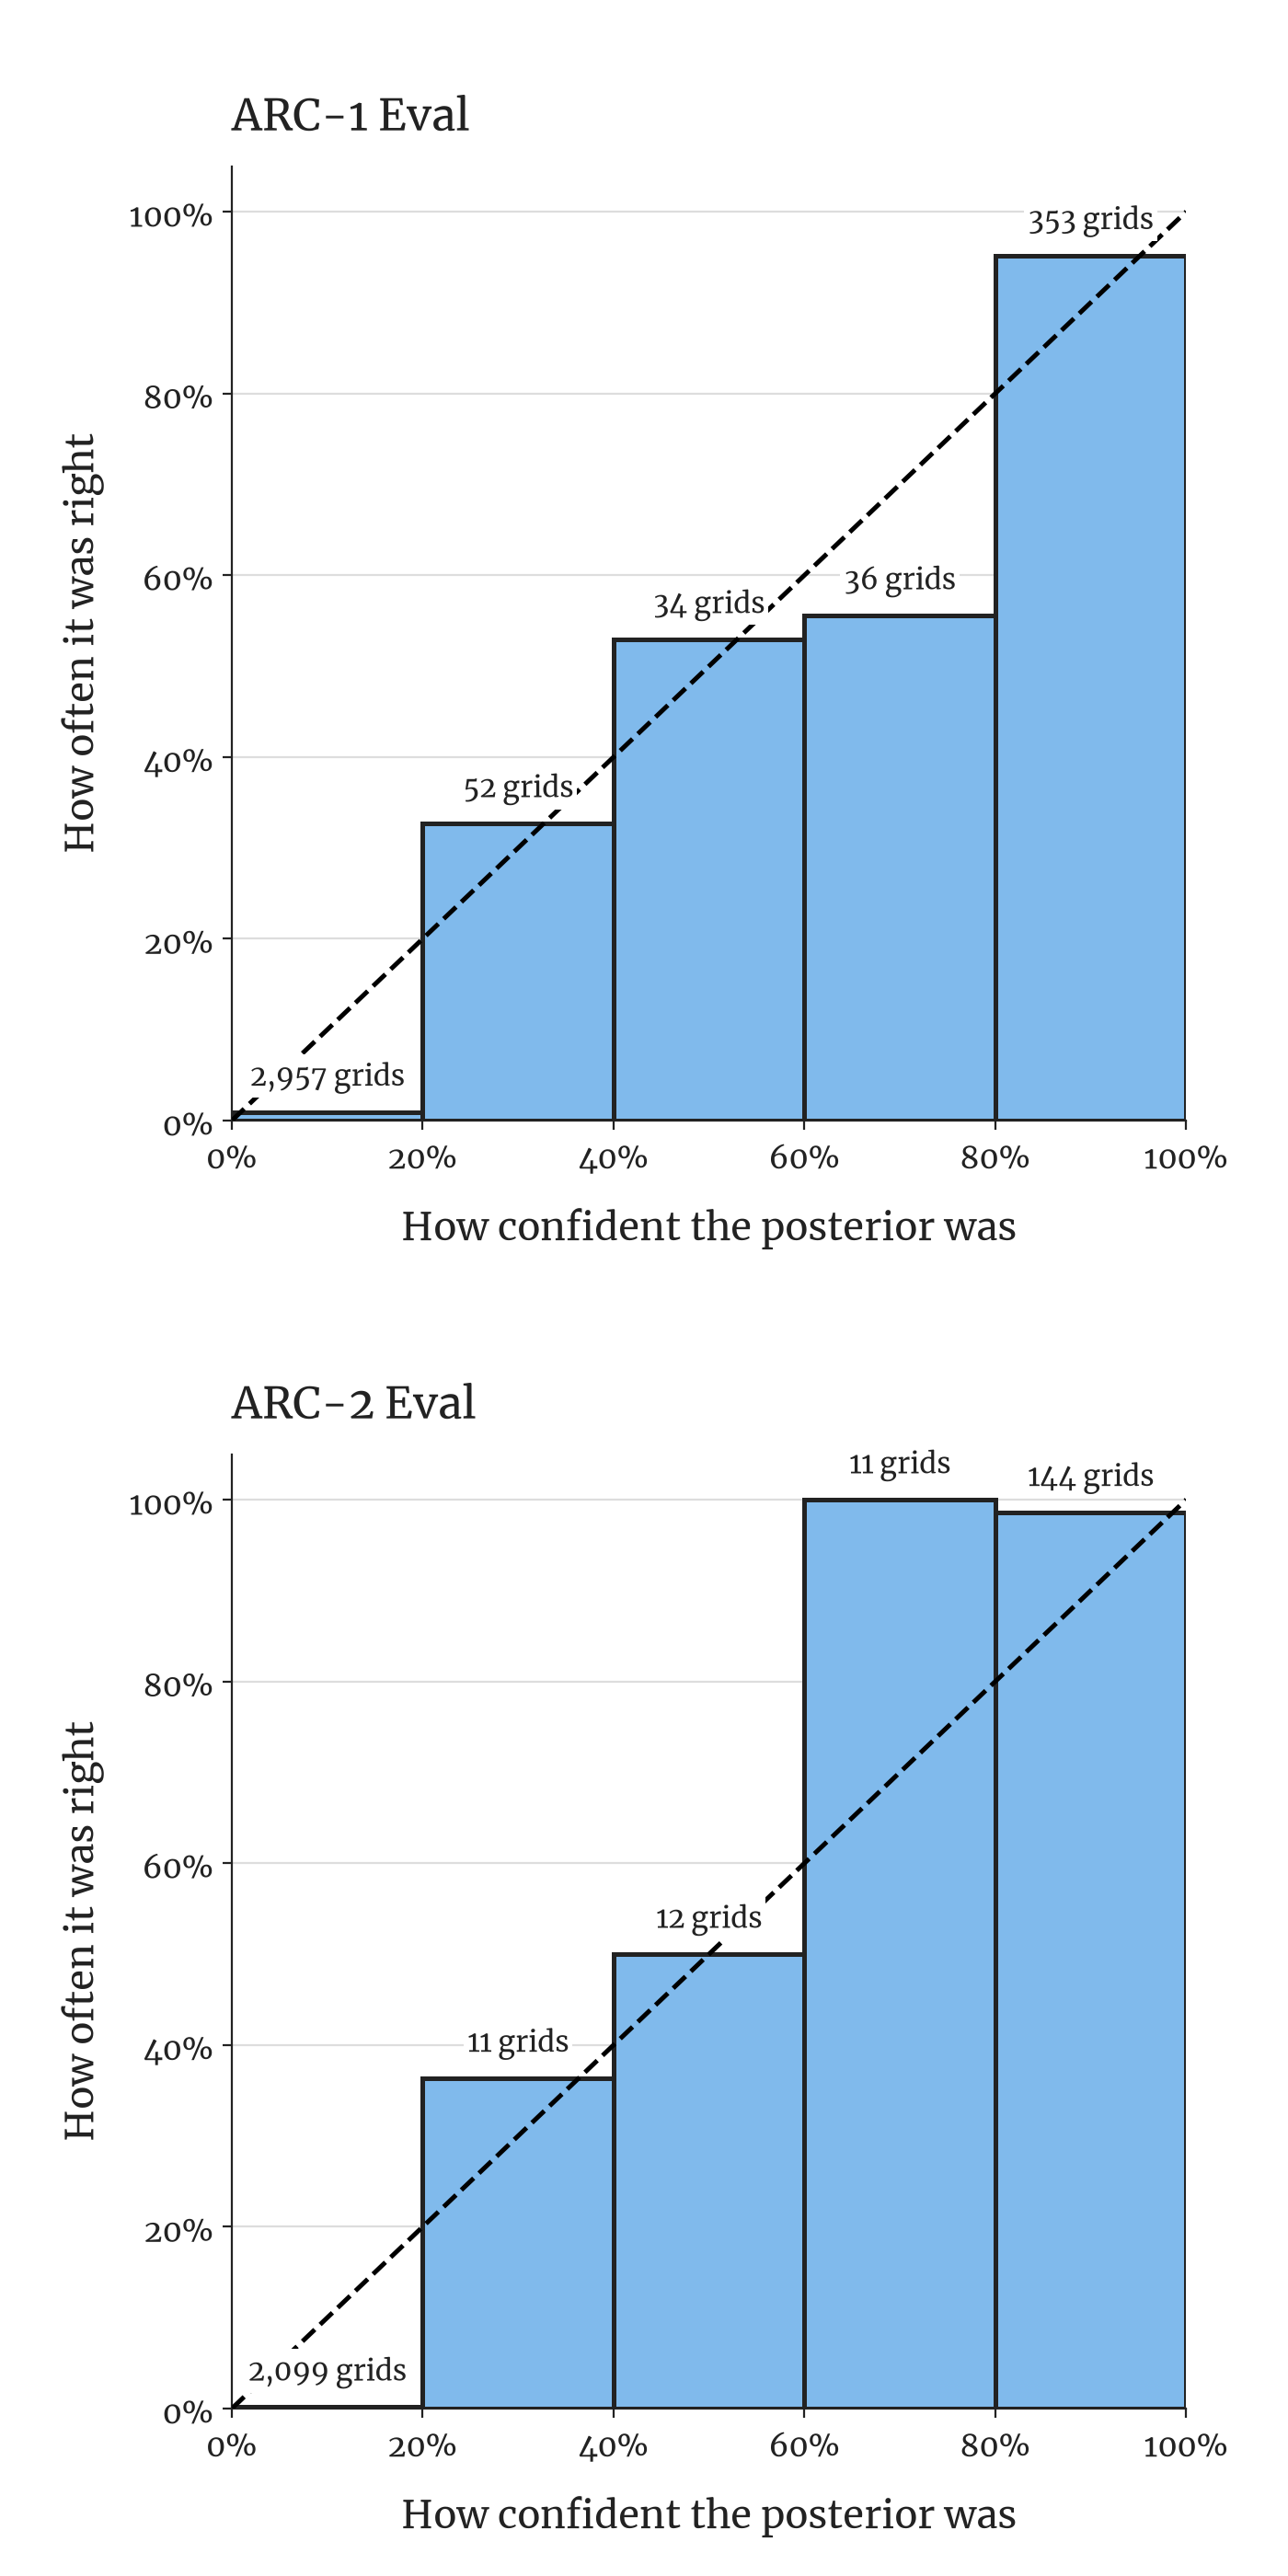
\includegraphics[width=\linewidth]{figures/dataviz/reliability.png}
    \caption{Reliability Diagram of AlexNot's approximate-Bayesian posterior (with ``out-of-model'' uncertainty) at predicting if a grid is the true answer.}
    \label{fig:reliability}
\end{figure}

As elaborated in \hyperref[sec:compression]{Understanding Is Compression}, AlexNot runs a softmax on all program scores (with a `dummy program' to stand in for ``out-of-model''/pseudo-Knightian uncertainty) to approximate a Bayesian distribution over programs \& predicted Test outputs. 

The good news: \textit{yes, AlexNot knows when it doesn't know.} Graphing the reliability diagram on both ARC-AGI-1/2 Public Evals (\autoref{fig:reliability}), it's well-calibrated: when it predicts an output-grid has an 80–100\% chance of being right, it in fact is 80–100\% of the time; likewise for 0–20\% and most other bins. You'll also notice it's bimodal: most of the time it's very sure an output is wrong, or very sure it's right, with little in the middle.

But the bad news: \textit{many true answers are in the middle.} For example, in \autoref{fig:alexnot_bayes}, AlexNot \textit{does} give the ground-truth answer as its most probable guess, but `only' at 57\% confidence, with 40\% confidence it never generated the true answer (out-of-model). This is because, on tasks where AlexNot \textit{does} find a program that fits all Demo pairs, $\sim$50\% of the time it doesn't generalize to Test. We could have made an ``overfit-ness'' detector, but we didn't invest time into that, since there was no contest penalty for giving a \textit{wrong} answer instead of saying ``I don't know''. Future Research for rule inducers (and any AI benchmark in general, really) should incentivize saying ``I don't know'' when it doesn't know, to reduce overconfidence \& hallucination.

Again: ``don't know'' is \textit{not} dangerous, only ``don't know \textit{that} you don't know''. AlexNot doesn't know when it has a true vs overfit solution, but it at least knows \textit{that.}

\subsection{Ablations/Variants to test the 3 Cognitive Science Principles}

The point of this project wasn't to get a high score (though that would've been really nice) but to investigate the 3 cognitive science principles: \textit{Understanding is Compression/Condensation, Problem-Solving (\& -Finding) is Search, Intuition is Pattern-Matching}. If our hypotheses are true, ablating parts of the compression-scores or the search algorithm should lead to huge drops in performance.

...we did not find that to be the case. See \autoref{fig:ablations_variants}.

\begin{figure*}
    \centering
    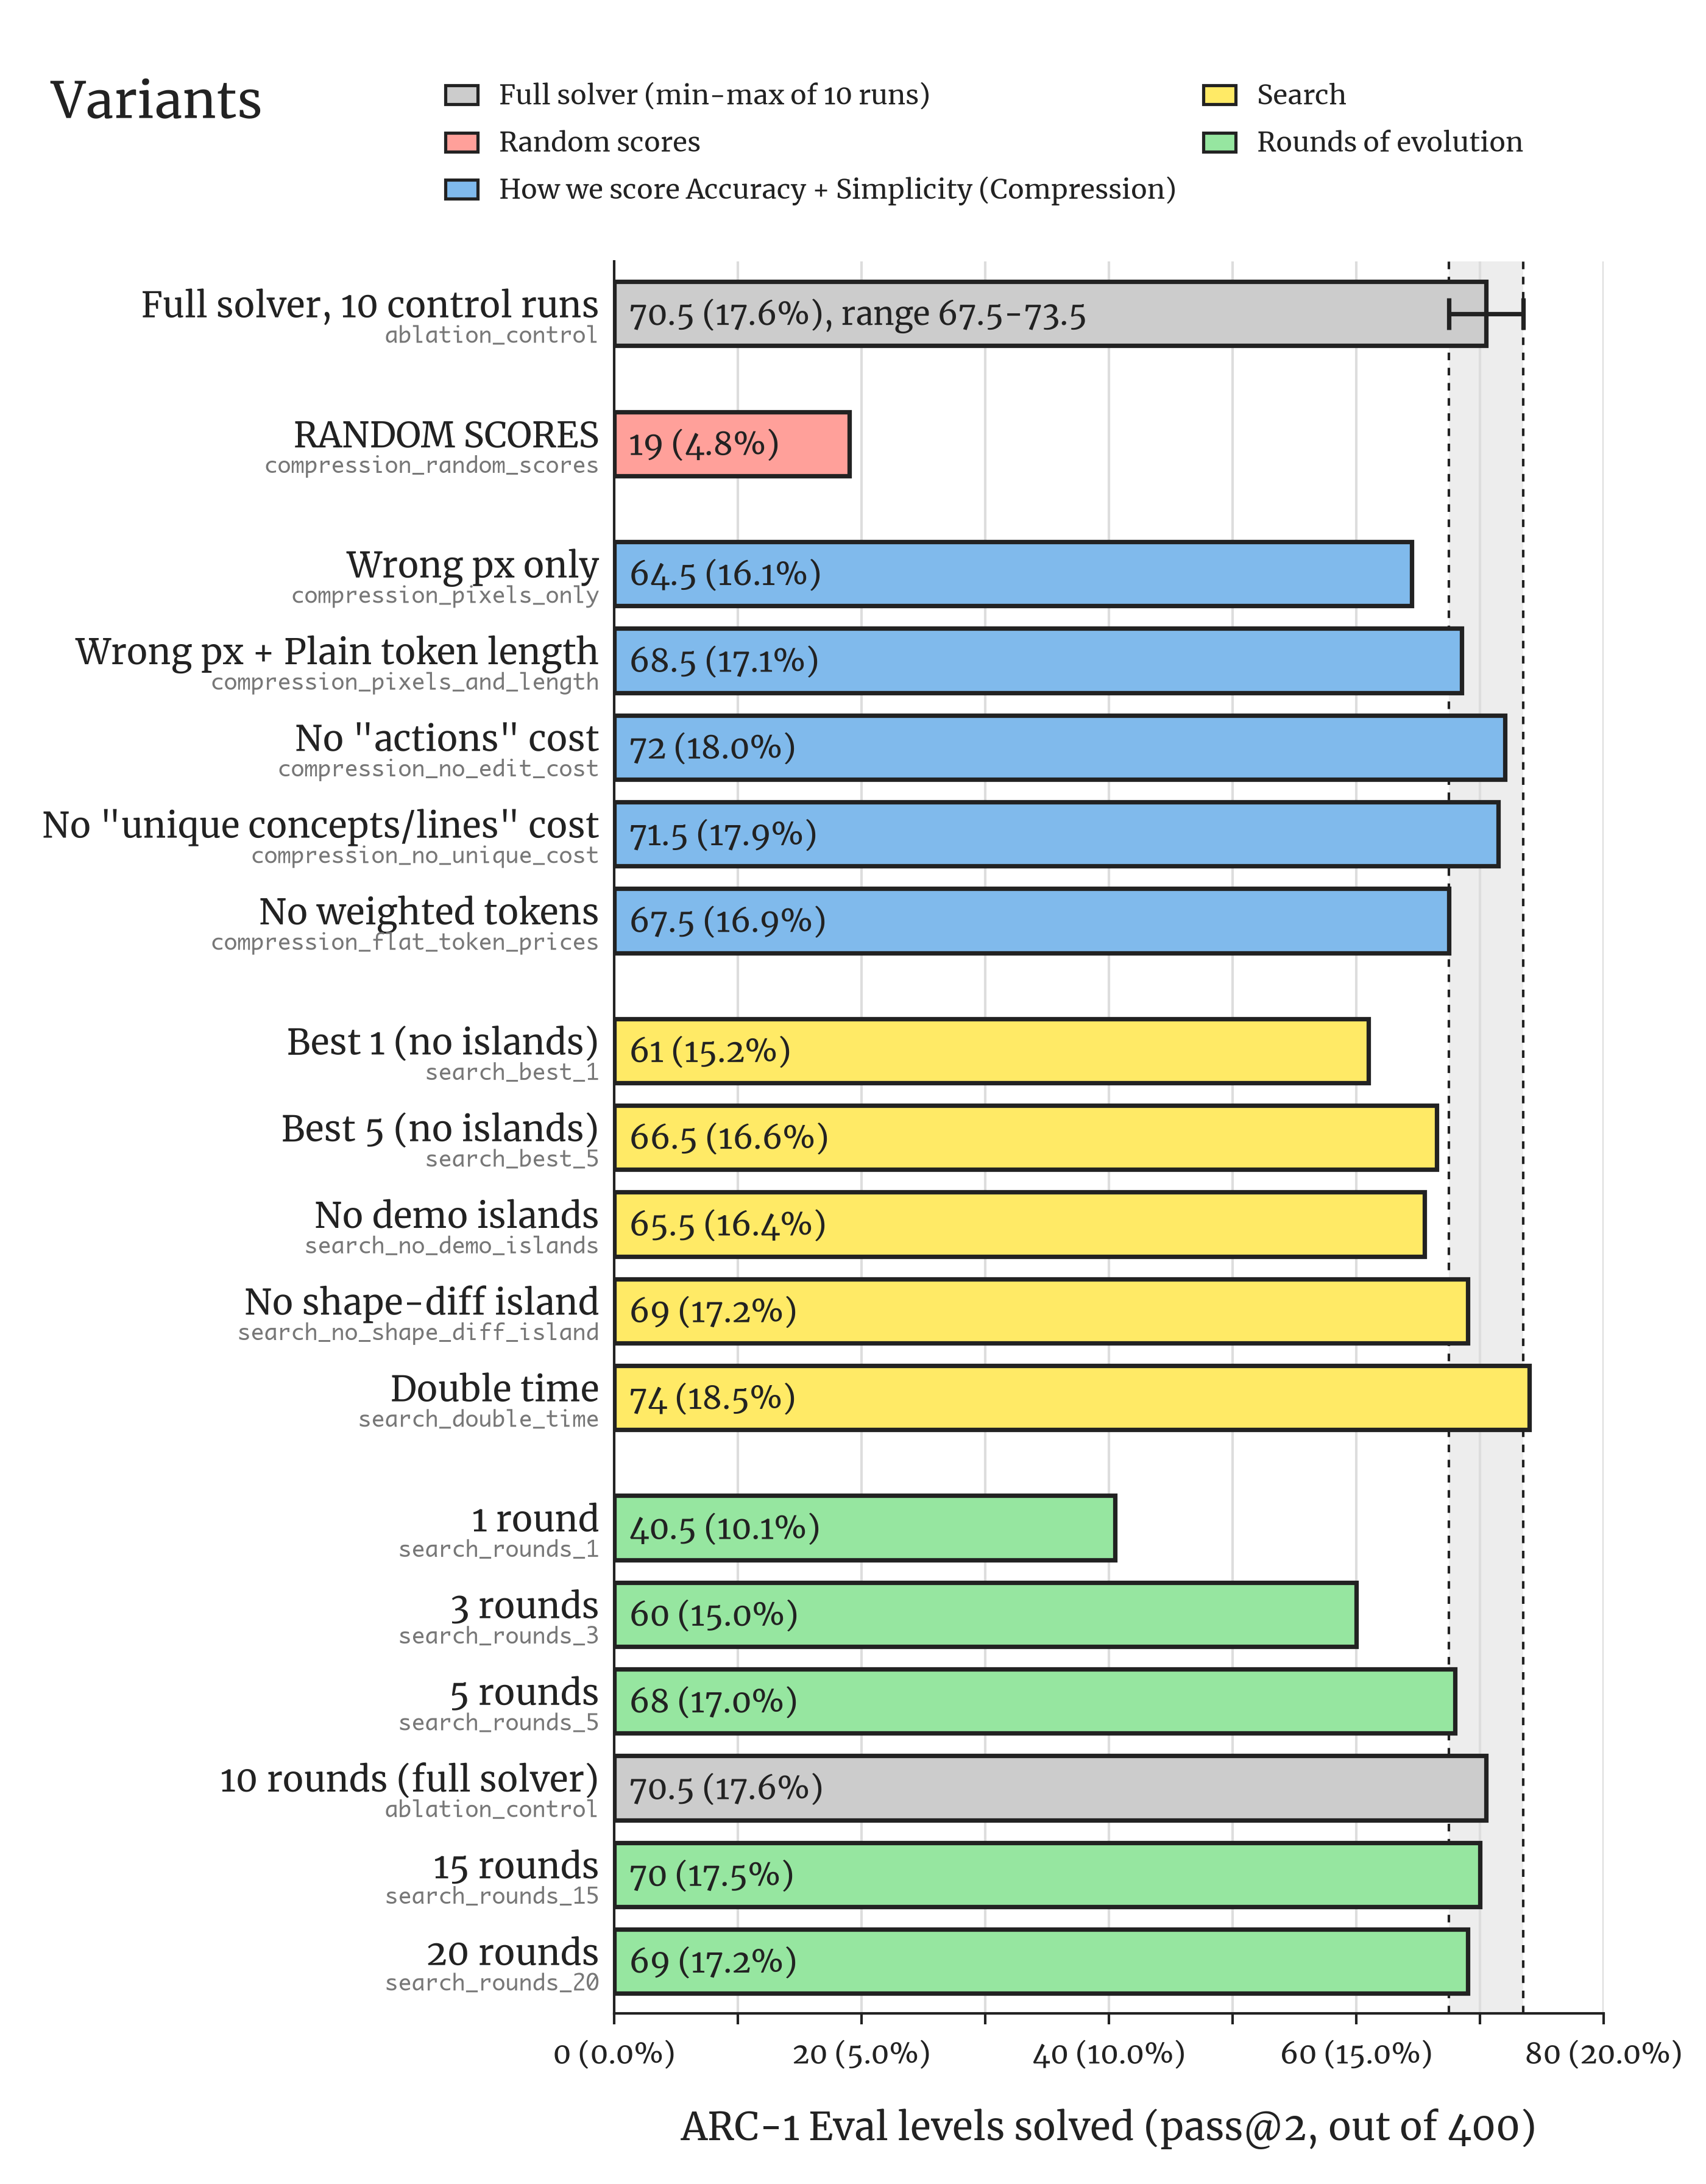
\includegraphics[width=\linewidth,height=0.95\textheight,keepaspectratio]{figures/dataviz/ablations.png}
    \caption{How every ablation/variant of AlexNot scores on ARC-AGI-1 Eval. Translucent gray bar shows the range from random seed luck alone, based on 10 control runs.}
    \label{fig:ablations_variants}
\end{figure*}

So... was this entire 60+ page paper based on a lie? \textit{Probably} not! Because we looked closer after getting a strange result: selecting \textit{only on pixel accuracy, not caring about program length}, led to only a small drop in performance. That \textit{can't} be literally true. ``If \texttt{[exact input grid]} then print \texttt{[exact output grid]}'' would have 100\% pixel accuracy on Demo pairs, but never generalize to Test. So, we tried two absurd ablations: what if we just went all the way, and just \textit{ablated scoring and evolutionary search entirely?}

As you can see in \autoref{fig:ablations_variants}, \textit{picking the winning program at random} still scored 1/4 as well, and doing \textit{no evolutionary search at all} (1 ``round'' of evolution, monkeys just propose programs from a blank parent, no further iteration) still did 1/2 as well.

How? \textbf{Because the power is in the starter pack, the priors \& heuristics.} The Core Prior monkeys were \textit{so} good at their task — monkey see, monkey suggest program — that at pass@2, they could \textit{still} solve a non-trivial number of tasks, \textit{even when we picked the winners at random, or ran only one round (no evolutionary search).}

So, we're counting this as suggestive evidence for our No Free Lunch-adjacent hypothesis, that we stated in \hyperref[sec:overview]{The Galaxybrained Overview}: \textit{the power of any search is mostly in its priors}. This does have the unfortunate side-effect, though, of making it hard to tell how important the individual elements of Compression or Search were, in absolute terms. So, looking only at the \textit{relative} drops in performance in \autoref{fig:ablations_variants}, we can say:

\begin{itemize}
    \item \uline{Compression}: Selecting for shorter programs \textit{is} better than accuracy alone. It's unclear if our ``naïve compression isn't enough'' hypothesis holds: none of the extra scoring terms, like fewer actions, or giving `natural' concepts lower cost, helped beyond seed noise. Still, anecdotally, as shown in \autoref{fig:beyond_compression}, they \textit{do} result in more human-like programs. (Even if it turns out ``inhuman'' programs generalized to Test at pass@2 anyway.)
    \item \uline{Search}: Having `islands' in our evolutionary search \textit{does} help, to avoid local minima, and encourage exploration. It's unclear if the high-level-prediction-error island, ``shape-diff'', helped. Double the wall clock time helped, but barely. More rounds of evolution help, with diminishing returns, no benefit past the default 10.
\end{itemize}

Finally, we'd like to \sout{brag} reiterate the cost efficiency of AlexNot: we could run 10 controls and 16 variants on 400 tasks each — 10,400 tasks altogether — \textit{for $\sim$\$2 USD in total on RunPod}.\footnote{It would've been \$0.35 if we'd used AWS's cheapest vCPU, t4g.nano.} So if you'd like to replicate \& extend our experiments, it'd be dirt cheap!

\begin{figure*}[h]
    \centering
    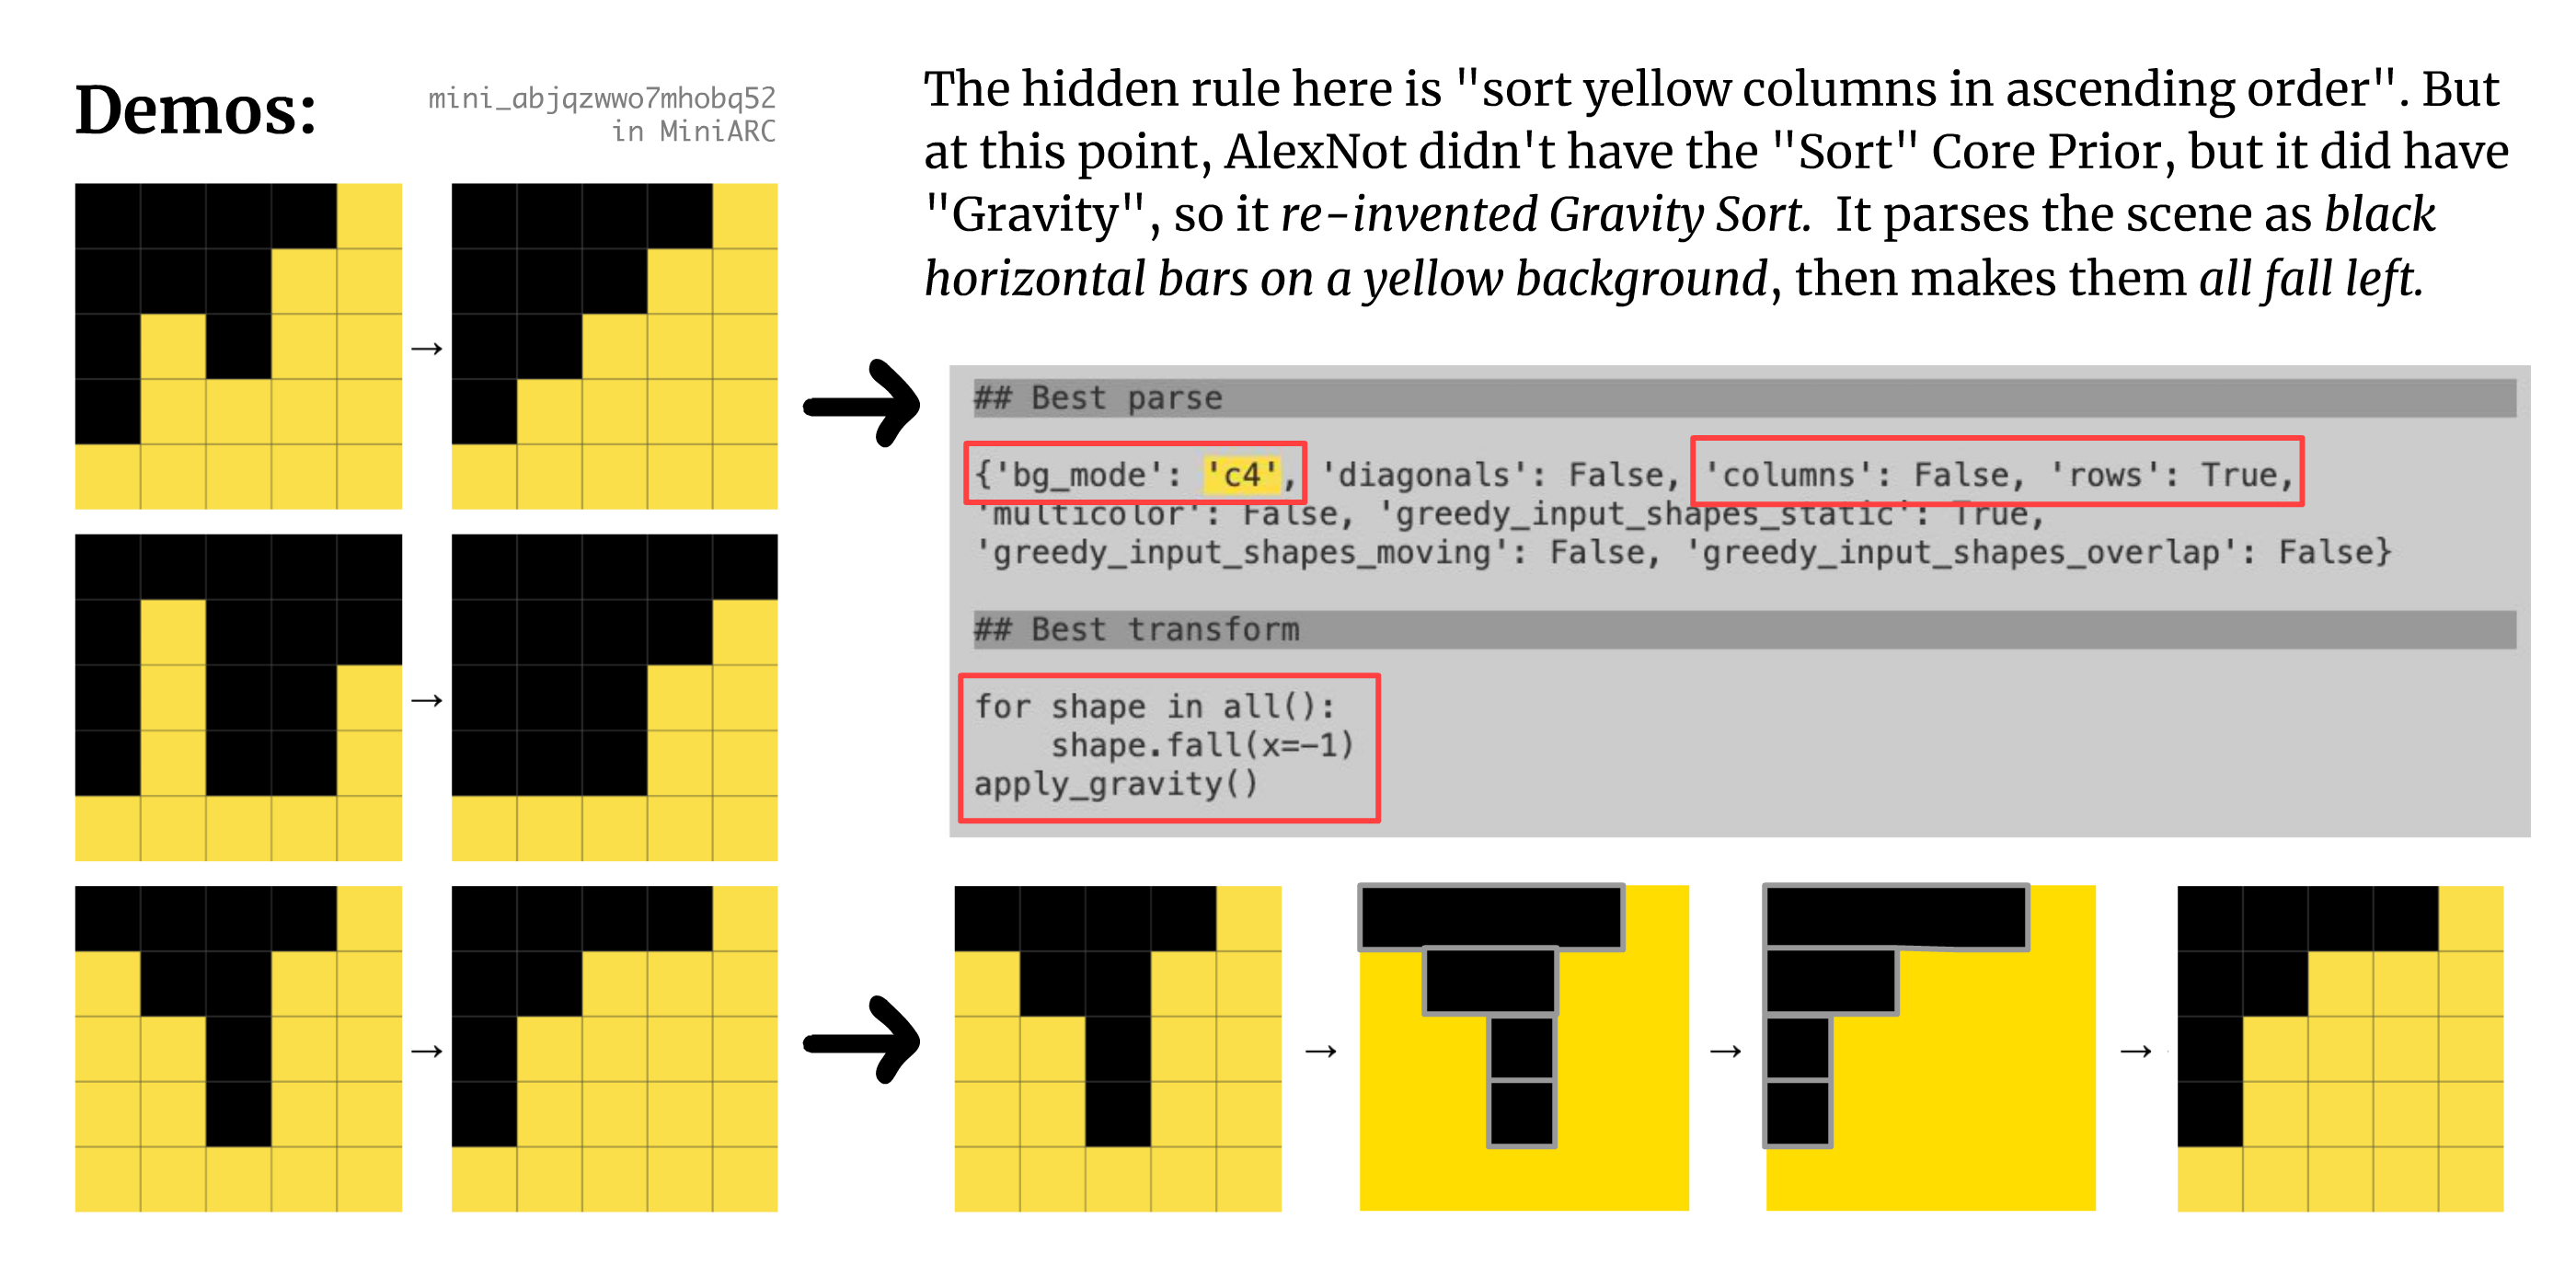
\includegraphics[width=\linewidth]{figures/across/gravity_sort.png}
    \caption{AlexNot re-inventing Gravity Sort}
    \label{fig:gravity_sort}
\end{figure*}

\subsection{A Cherry-Picked Anecdote of Open-Ended Invention}

Early on in development, we didn't have the ``sorting'' Core Prior in the DSL and code-generating monkeys, but we \textit{did} have the ``gravity'' Core Prior. On one specific level in Mini-ARC, AlexNot was able to solve a ``sort these elements'' task anyway, by \textit{re-inventing Gravity Sort} \citep[a.k.a.\ Bead Sort;][]{bead_sort}, a physical-mechanical sorting algorithm that runs in $O(\sqrt{n})$ time.\footnote{Because the time it takes for elements to fall $n$ ranks under real-world gravity is proportional to $\sqrt{n}$. Gravity Sort is \textit{not} a comparison-based sorting algorithm, and only works when all elements are positive integers, hence why the $O(n \log n)$ lower bound doesn't apply.} (\autoref{fig:gravity_sort})

\textit{After} we implemented the ``sorting'' Core Prior, AlexNot started reliably solving this puzzle the intended way. Still, as cherry-picked as this may be, this \textit{is} an example of AlexNot re-inventing a real, academically-published sorting algorithm from scratch. A general lesson for open-ended innovation: creative ``jumps'' often come from odd constraints!

\subsection{AlexNot-ODE: inducing real equations from noisy sparse data}

Finally, the most exciting experiment we did on AlexNot!

ARC-AGI is a good benchmark, because it's ``science in miniature'': observe sparse data, induce/abduce the hidden rule, apply it. But it deviates from real-world observational science in a few important ways: it has pixel-perfect data, the hidden rules are deterministic, and there's no data \textit{across} time, just before/after pairs. (ARC-AGI-3, their first interactive benchmark, \textit{does} address that last concern.) Again, this is 100\% fine for ``the MNIST of fluid intelligence'' — nobody complains that MNIST has no circuit diagrams — but wouldn't it be nice to try it with abducing \textit{real-world} scientific theories, from noisy, sparse time-series data?

We present \textsc{AlexNot-ODE}, which does exactly that! We vibe-coded this with Claude in one (1) day. We mention that to illustrate a) how modular and easy-to-repurpose AlexNot's architecture is, b) how an LLM can easily work \textit{with} an AlexNot-style harness; more details on this idea in the \hyperref[sec:limitations]{Future Research} section.

(AlexNot-ODE's code is at \url{https://github.com/ncase/alexnot-ode}.)

\begin{figure*}[h]
    \centering
    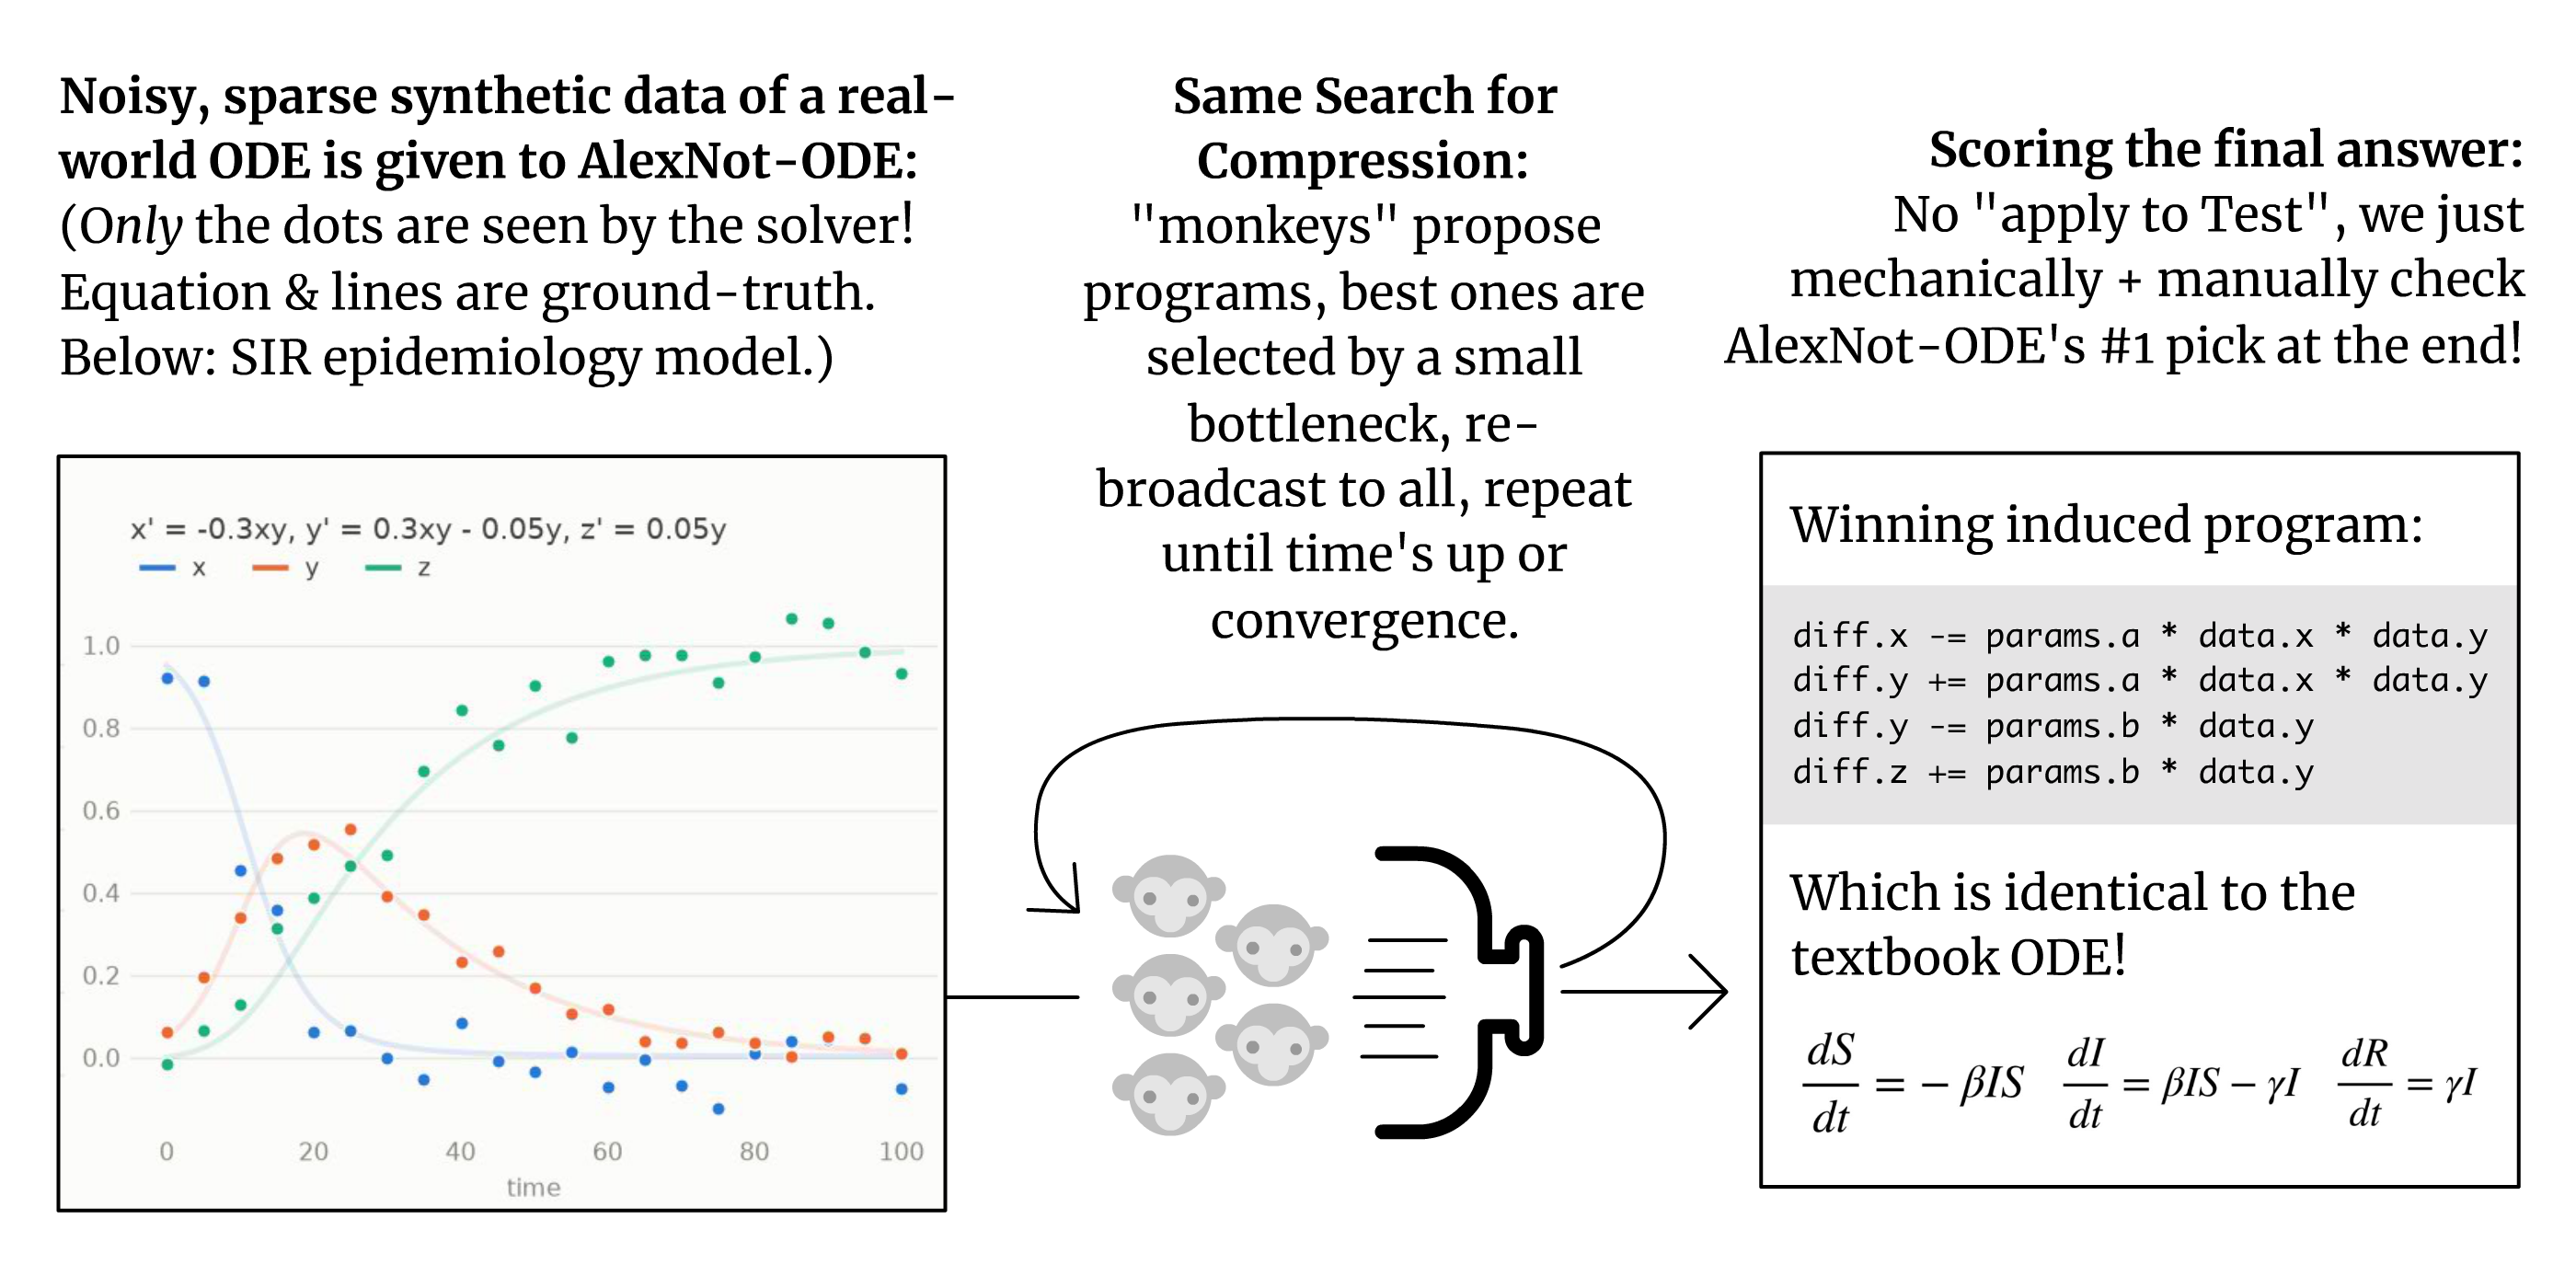
\includegraphics[width=\linewidth]{figures/across/alexnot_ode.png}
    \caption{Full schematic of the minimalist AlexNot-ODE core loop.}
    \label{fig:alexnot_ode}
\end{figure*}

AlexNot-ODE uses the same design principles as AlexNot: (See \autoref{fig:alexnot_ode})

\begin{enumerate}
    \item Select the symbolic representation (ODE/ordinary differential equation) that best compresses (least squares error + fewest tokens + fewest free-parameters) the data,
    \item via an evolutionary search,
    \item guided by pattern-matchers.
\end{enumerate}

Those pattern-matching ``monkeys'' are:

\begin{itemize}
    \item Suggest a linear fit
    \item Suggest a quadratic fit
    \item Add random single terms
    \item Delete random interaction terms
    \item Delete random lines
    \item Delete terms whose coefficient is near 0
    \item Delete coefficients close to $\pm1$
    \item Unify parameters. (e.g. if $a \approx b$ , try replacing $a$ with $b$.)
    \item Find \& replace arithmetic coincidences. (e.g. if $a \approx b + c$, try replacing $a$ with $b + c$.)
\end{itemize}

At solve time, AlexNot-ODE is fed noisy, sparse time-series data (synthetically generated at various levels of noise), and the solver induces the simplest equation that explains that data. (Unlike ARC-AGI-1/2, we don't check by applying it to Test data: we directly check if the program is equivalent to the intended answer, both mechanically and manually.)

The 8 different equations we tried come from physics, life sciences, and business. In roughly ascending order of complexity:

\begin{itemize}
    \item Exponential growth/decay (Physics)
    \item Newton's law of cooling (Physics)
    \item Logistic growth (Ecology)
    \item Bass diffusion model of advertising \& word-of-mouth (Business)
    \item Falling object with air drag (Physics)
    \item Damped harmonic oscillator (Physics)
    \item Lotka-Volterra predator-prey model (Ecology)
    \item Susceptible–Infected–Recovered (SIR) model (Epidemiology)
\end{itemize}

At 10\% noise, AlexNot-ODE could induce the correct equation on 90+\% of runs (for each equation). Even at 20\% noise, AlexNot-ODE could still recover most of them, including the complex Damped Oscillator, Lotka-Volterra predator-prey, and SIR epidemiology models. (And again, at high efficiency: mere CPU-seconds per task.)

Secondary results: AlexNot-ODE could recover the famous \textit{chaos theory} ODE, the Lorenz equations/``chaos butterfly'', 10+\% of the time, at 10\% noise. AlexNot-ODE was also able to \textit{partly} recover the Lotka-Volterra predator-prey equations \textit{from real-world Canadian lynx \& hare data}. \citep{lynx_hare_stan} (AlexNot-ODE's failure was that, by coincidence, if one were to directly fit Lotka-Volterra to that data, $\beta$ and $\delta$ (predator \& prey's interaction coefficients) end up being similar, and $\gamma$ (predator death rate) is close to 1: so, for the sake of compression, AlexNot-ODE incorrectly merges $\beta$ and $\delta$, and drops the $\gamma$ coefficient.)

To be clear, the above ODEs are simple enough that you can just discover them with plain SINDy \citep{sindy}, or even brute-force search. But SINDy can't generalize from ODEs to ARC-AGI, while AlexNot's architecture \textit{does} generalize from ARC-AGI to ODEs from real-world sciences. Our 1-day vibe-coded AlexNot-ODE is just a proof-of-concept that the core principles of fluid intelligence \textit{work} — compress, search, pattern-match, repeat — and they \textit{can} generalize to LLM-symbolic collaboration, and real-world scientific use.

Speaking of which, it's now time for the Future Research section...




%%%%%%%%%%%%%%%%%%%%%%%%%%%%%%%%%%%%%%%%%%%%%%%%%%%%%%%%%%%%%%%%%%%%%%%%%%%%%%%%%%%%%%
%%%%%%%%%%%%%%%%%%%%%%%%%%%%%%%%%%%%%%%%%%%%%%%%%%%%%%%%%%%%%%%%%%%%%%%%%%%%%%%%%%%%%%
% LIMITATIONS & FURTHER RESEARCH
%%%%%%%%%%%%%%%%%%%%%%%%%%%%%%%%%%%%%%%%%%%%%%%%%%%%%%%%%%%%%%%%%%%%%%%%%%%%%%%%%%%%%%
%%%%%%%%%%%%%%%%%%%%%%%%%%%%%%%%%%%%%%%%%%%%%%%%%%%%%%%%%%%%%%%%%%%%%%%%%%%%%%%%%%%%%%

\section{Summary, Limitations, Future Research}\label{sec:limitations}
\begin{quote}
To discover what deep learning is missing, let's see how far we can go with deep learning \textit{missing.}

— us, an hour ago, at the top of this paper
\end{quote}
In summary, here's what we learnt from our minimalist experiment in tackling ARC-AGI; no neural networks, just applying the core principles of cognitive science as directly as possible:

\begin{itemize}
    \item \textbf{Theory \textit{works!} (mostly.)} $\Rightarrow$ On ARC-AGI-2 Public Eval, our pure-symbolic solver is on par with last year's Top 3 pure-neural solvers, but \textit{over 5,000$\times$} more efficient.
    \item \textbf{Understanding is Compression/Condensation} $\Rightarrow$ We found suggestive evidence that \textit{simplicity is not enough} for generating human-like rules, so we added priors for `fewer actions', `fewer concepts', `fewer free parameters', and `natural-ness'. (\hyperref[sec:results]{Results \& Experiments} did not find these helped on raw pass@2 score, but looking at individual tasks, they \textit{do} help make the winning program more human-like.) It's obvious in hindsight, but if the purpose of simplicity is generalization, why not select for \textit{everything} that predicts generalization?
    \item \textbf{Problem-Solving (\& -Finding) is Search} $\Rightarrow$ AlexNot's GWT-inspired evolutionary search was always the main plan, but we didn't expect how important the \textit{Causality/Bongard} search would be. This let each monkey ask: what properties X,Y caused some things to do Z, while the other things didn't?
    \item \textbf{Intuition is Pattern-Matching} $\Rightarrow$ Finally, we were surprised that pure-symbolic heuristics had some intrinsic advantages over pure-neural: the ability to do explicit search, and higher speed/sampling + higher useful variance = better best-of-N performance.
\end{itemize}

With all that said, it is now time to report the greatest limitation we found, in attempting a pure-symbolic approach:

\textit{Holy SHIT that was tedious.}

Not as tedious as Cyc — which, by 2002, took \$60 million and 600 person-years to hand-write millions of ``common-sense axioms'' — but yes, there's a reason no major modern AI product is pure-symbolic. Every other limitation of AlexNot is downstream of its creation process being finicky and effort-intensive:

\begin{itemize}
    \item AlexNot's DSL is not Turing-complete. It doesn't even have if-then statements.
    \item All coefficients and hyperparameters were manually tuned.
    \item AlexNot \textit{knows} when it doesn't know... but it often doesn't know (if a solution it has is real vs overfit).
    \item The core search is simple — it's just evolutionary search — but the add-ons strike us as inelegant. Specifically, AlexNot must parse the scene \textit{before} annotating details \textit{before} searching for the hidden rule, instead of what humans can do: flexibly move between any stage of search.
    \item We ran out of time to implement all plausible human-universal Core Knowledge Priors, which again, nobody knows the full true list of, but there may be dozens of categories and 100–200 sub-categories. In contrast, by our rough count, we only implemented $\sim$50 sub-categories.
\end{itemize}

Sure, 1–2 hundred is far better than Cyc's millions, and given how evolution took 3.7 billion years to create \textit{us}, there's likely \textit{some} fine-tuned ingredients behind human general intelligence. But there's \textit{got} to be a better way! That's what Neuro-Symbolic AI promises: the lack of rigorous causal models in neural approaches can be filled by symbolic reasoning, and in return, symbolic's manual tediousness can be filled by neural learning.

So while \textit{pure-symbolic} AlexNot should not be extended, the rest of this section will sketch some future research ideas, on how to apply the modular architecture design and Cognitive Science principles behind AlexNot \& AlexNot-ODE, towards:

\begin{figure*}
    \centering
    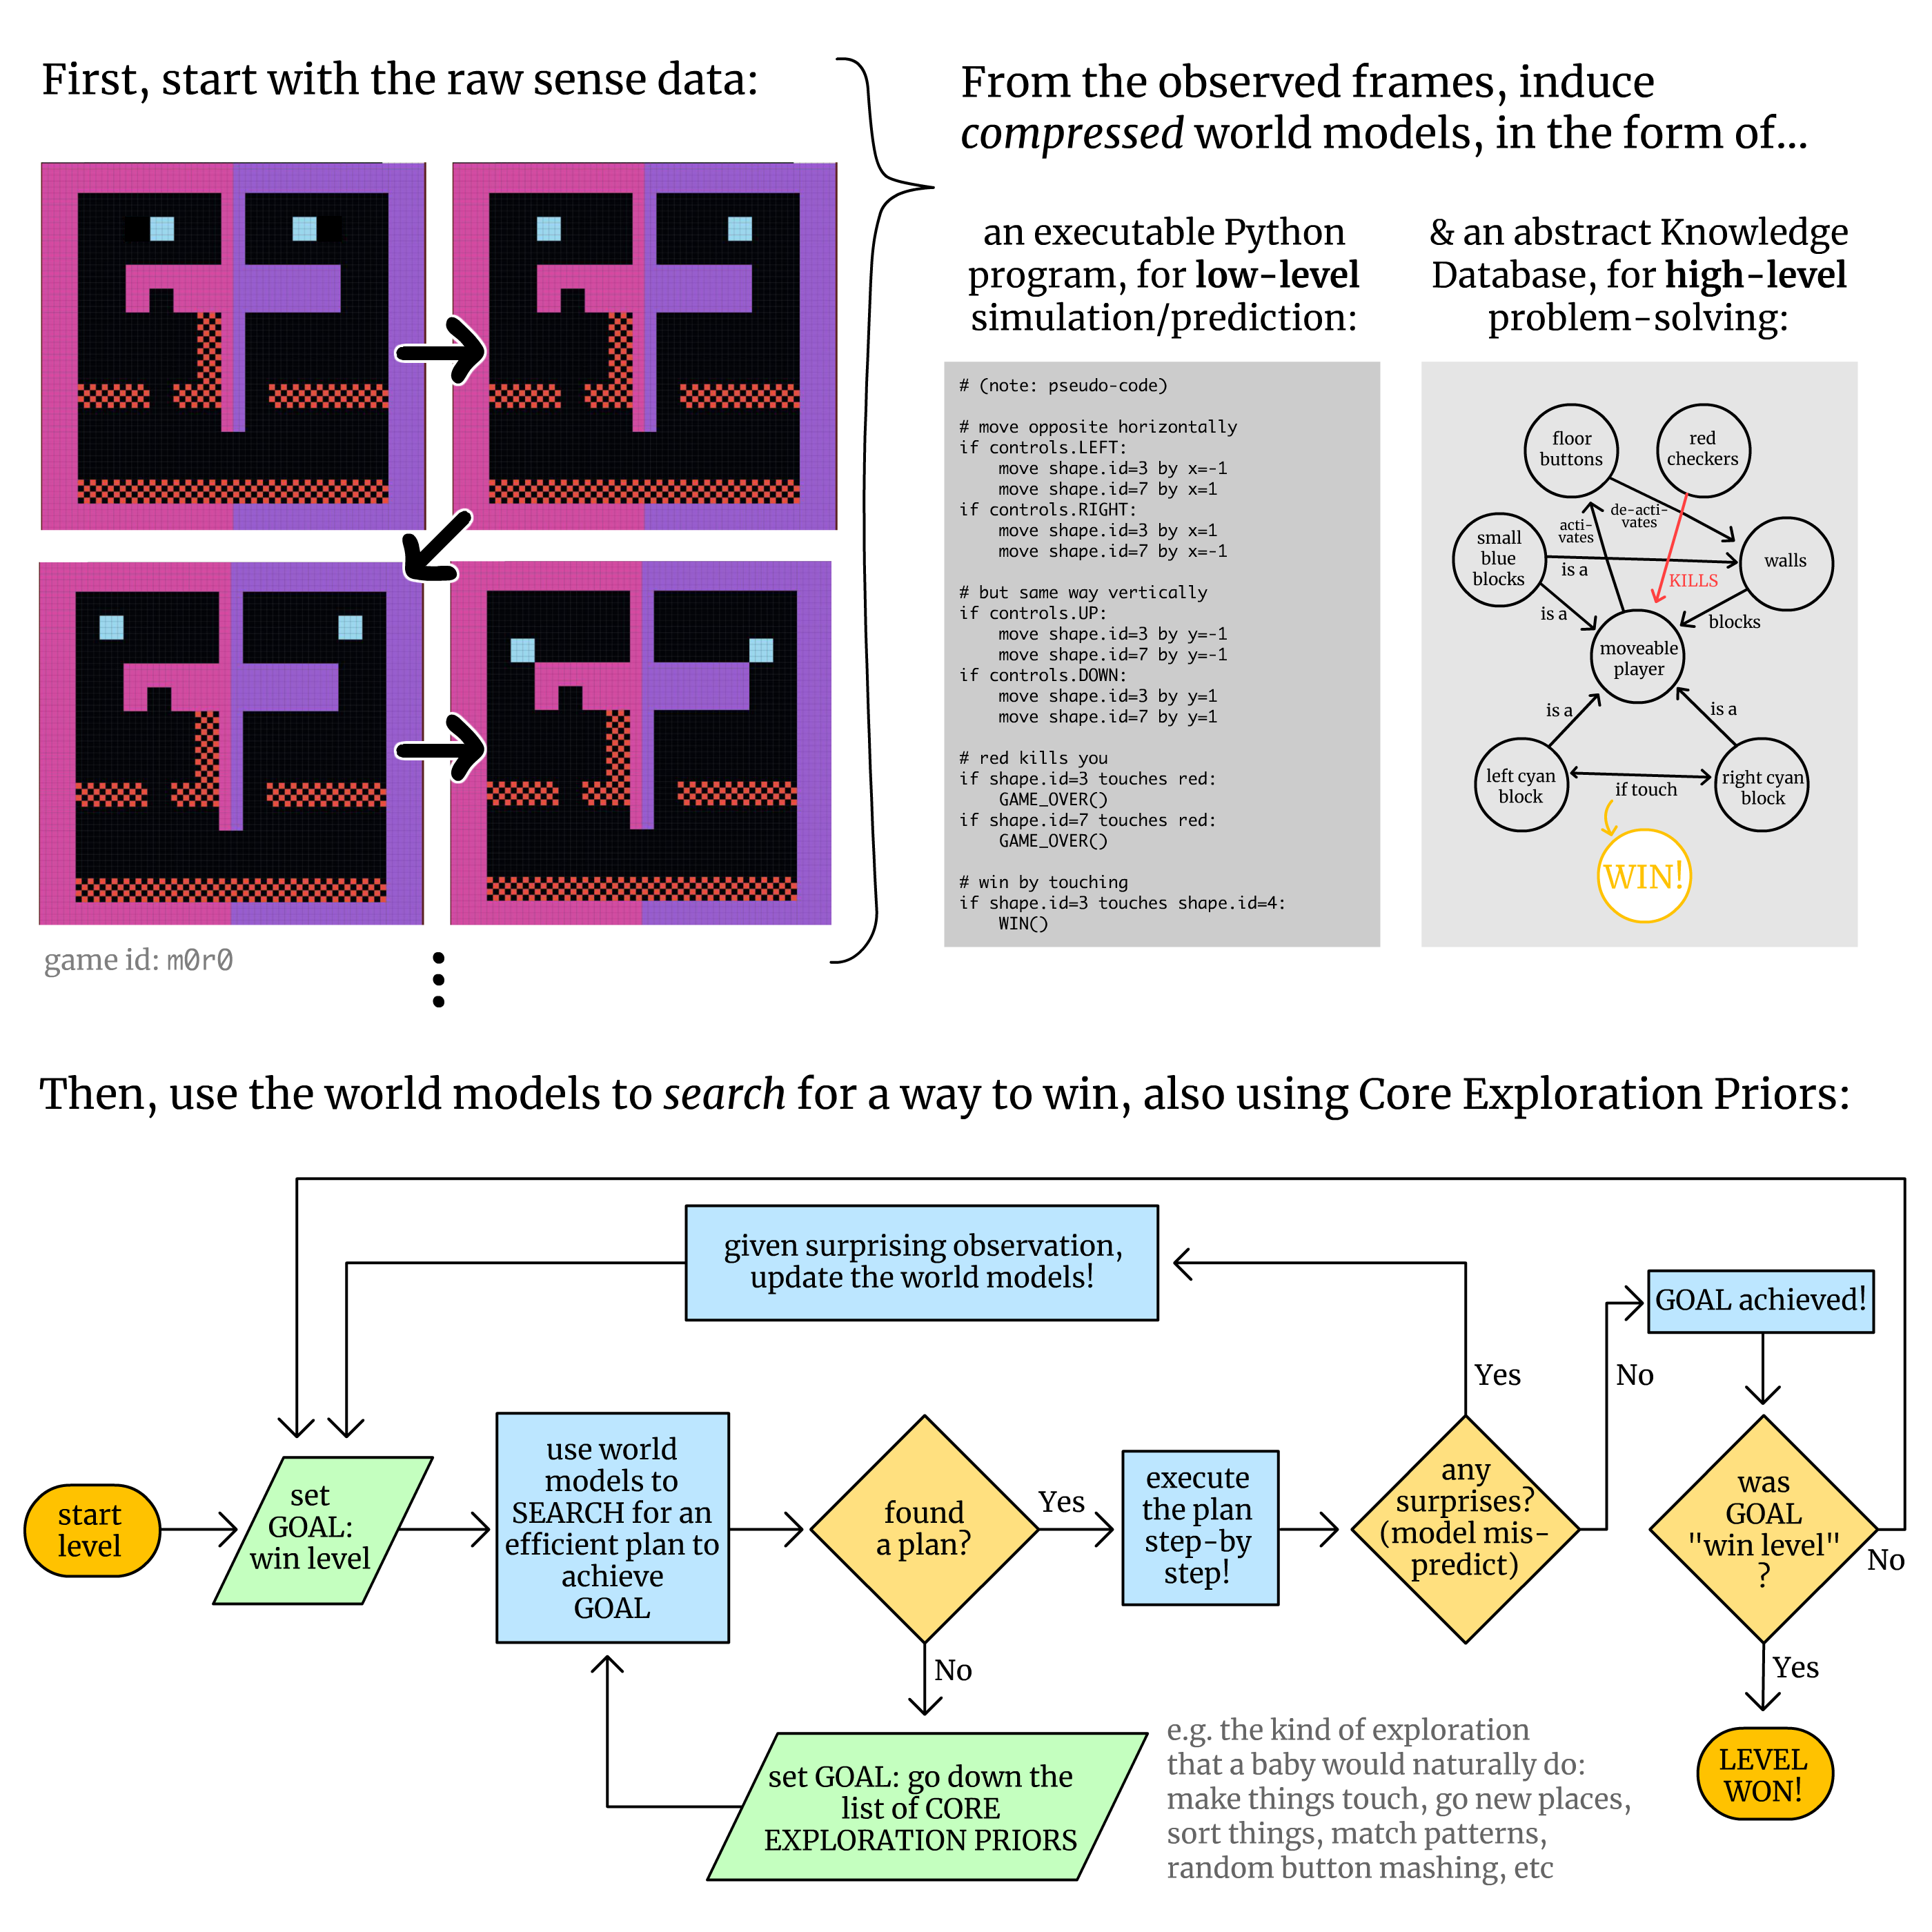
\includegraphics[width=\linewidth]{figures/across/arc_3.png}
    \caption{Design sketch for how a Cognitive Science-inspired solver for ARC-AGI-3 (and -4?) could work.}
    \label{fig:arc_3}
\end{figure*}

\begin{enumerate}
    \item Progress on ARC-AGI-3 (agentic intelligence) and ARC-AGI-4 (open-ended innovation).
    \item Ways to make LLMs \textit{convert themselves} into Neuro-Symbolic hybrids, in a way that's ``business-incentive-gradient-compatible'': \textit{every step} in the transition makes for a more profitable product.
    \item A ``Unix Philosophy for AGI'' or ``Peer-to-Peer AGI'', and discussion on how (Neuro-)Symbolic AI could be a win-win-win: boosting AI Capabilities/Abundance, AI Safety/Security, \textit{and} fighting the concentration of power in AI.
\end{enumerate}

\subsection{Advancing on ARC-AGI-3 and -4}

\textbf{ARC-AGI-3 (agentic intelligence):}

Originally, we also planned to tackle the ARC-AGI-3 videogames, by wrapping AlexNot in a simple harness. (See \autoref{fig:arc_3})

First, feed all frames of the videogame to AlexNot, so it can induce a symbolic, causal world model for the game, as an executable Python program. Maybe also induce an abstract Knowledge Graph, for higher-level planning. (Plain AlexNot does not handle time-series data, but AlexNot-ODE does. Either way — as the vibecoded-in-a-day AlexNot-ODE showed — AlexNot's modular architecture makes it easy to repurpose it for almost any model-induction task.) 

Next, we simply apply a portfolio of classic planning algorithms, like A* and means-ends analysis, to these world models, to win the level! If no plan is found, fall back to (what we were going to call) ``Core Exploration Priors'': the kinds of exploration that — to many parents' chagrin — human toddlers universally do: mash buttons, touch random things, go somewhere they haven't before, sort things, match things, make things hit other things, etc. This would let an agent efficiently find new interesting states, and whenever a prediction error happens, it can learn from the surprise, update/re-induce its world models, and try again to win.

(Another benefit of AlexNot discovering not just one best world model, but an approximated Bayesian ensemble, is that it \textit{could} better balance exploration/exploitation, and even do optimal experiment design to best distinguish between world models. See \citet{empa}'s EMPA (Exploring-Modelling-Planning Agent) for a proof-of-concept of a Bayesian world-modelling AI that efficiently learns to play novel videogames.)

While we never got to try this (see: how tedious making a pure-symbolic AI is) we're fairly confident \textit{some} variant of the above plan would work for getting $\sim$100\% on ARC-AGI-3, given that that's what pretty much every frontier-LLM-with-harness that got $\sim$100\% on ARC-AGI-3 already did \citep{hill_climbing_arc_3,prolong_arc_3,retrodict_arc_3,astra_arc_3}.

\textbf{ARC-AGI-4 (open-ended innovation):}

ARC-AGI-4 \textit{has no official preview at the time of this writing}, so all the following is wild speculation off the ARC founders' Xeets. All that's publicly announced about ARC-AGI-4 is that it'll target ``open-ended innovation'' \citep{arc_agi_4_announcement}. We also know the tasks will be interactive, and — in line with the spirit of the ARC benchmarks — rely \textit{only} on the universal Core Knowledge Priors, while remaining ``easy/fun for humans, hard for (current) AI''.

\begin{figure}[t]
    \centering
    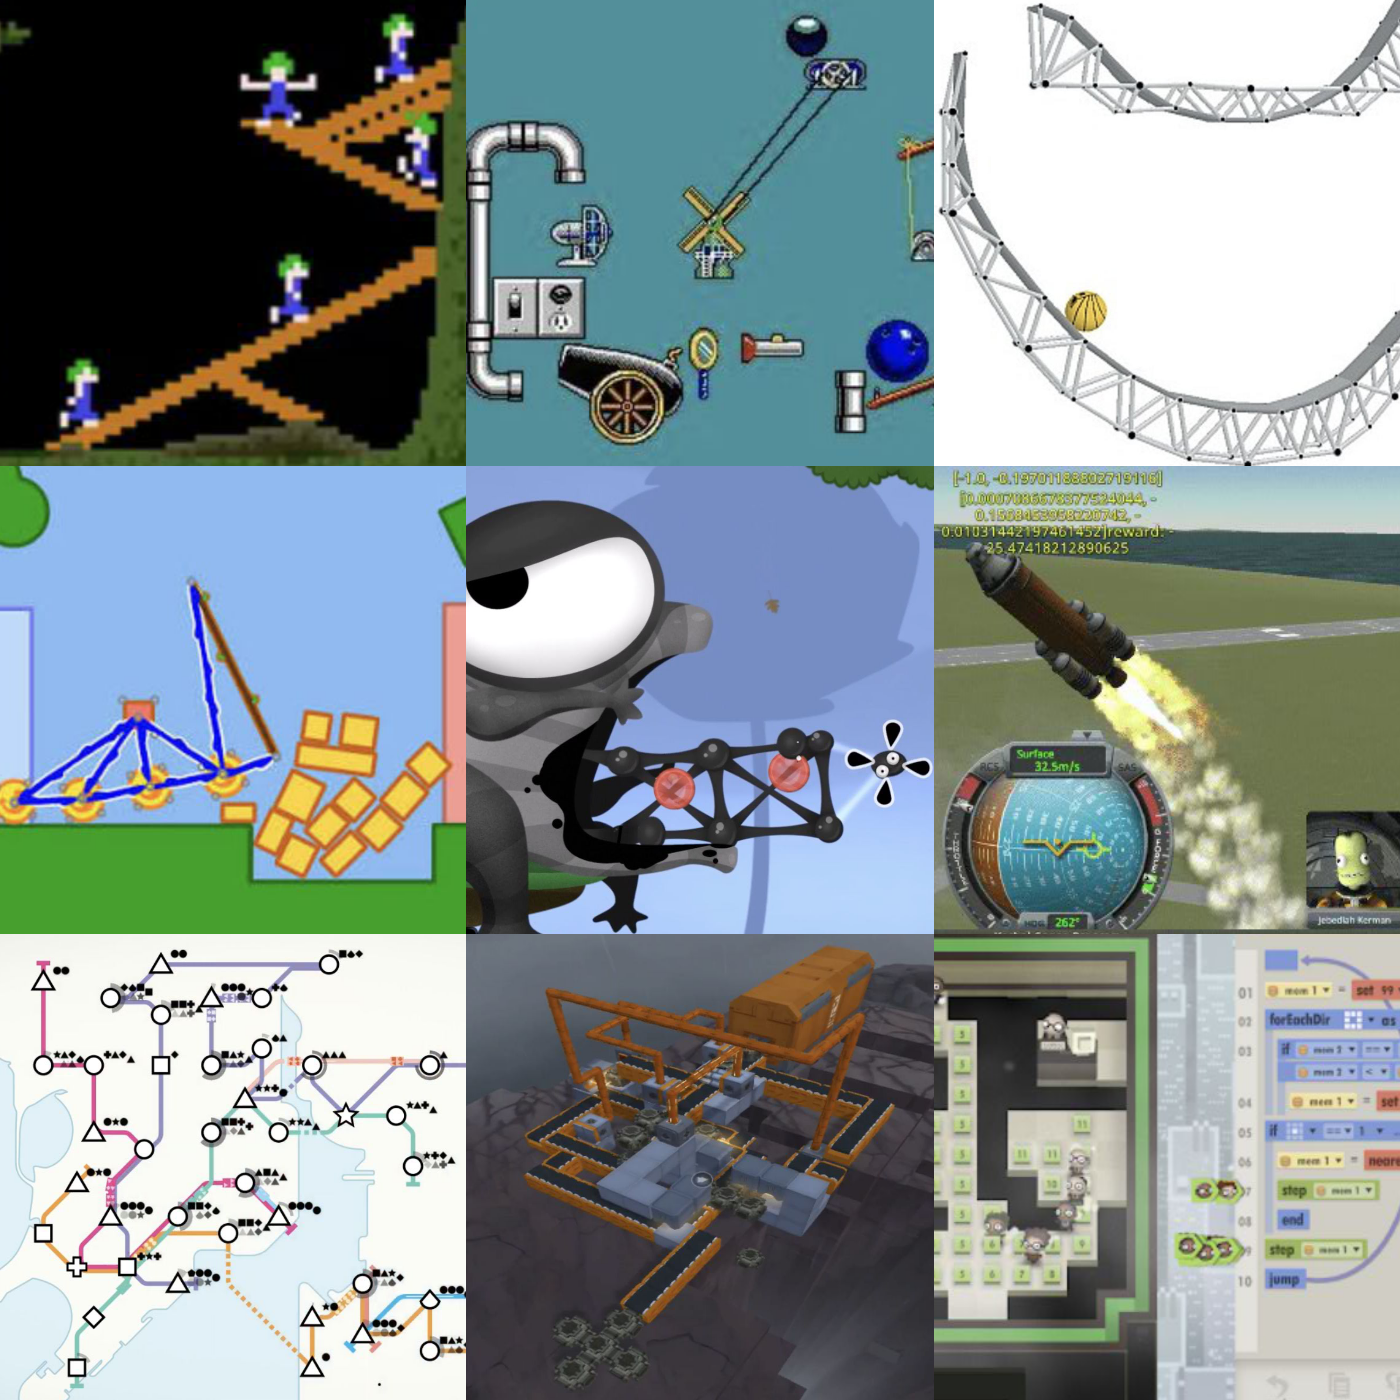
\includegraphics[width=\linewidth]{figures/mini/nostalgia.png}
    \caption{Examples of classic videogames featuring \textit{open-ended innovation}. This Figure exists primarily for nostalgia value. In reading order: \textit{Lemmings} (1991), \textit{The Incredible Machine} (1993), \textit{Armadillo Run} (2006), \textit{Fantastic Contraption} (2008), \textit{World of Goo} (2008), \textit{Kerbal Space Program} (2011), \textit{Mini Metro} (2014), \textit{Infinifactory} (2015), \textit{7 Billion Humans} (2018).}
    \label{fig:nostalgia}
\end{figure}

\begin{figure*}
    \centering
    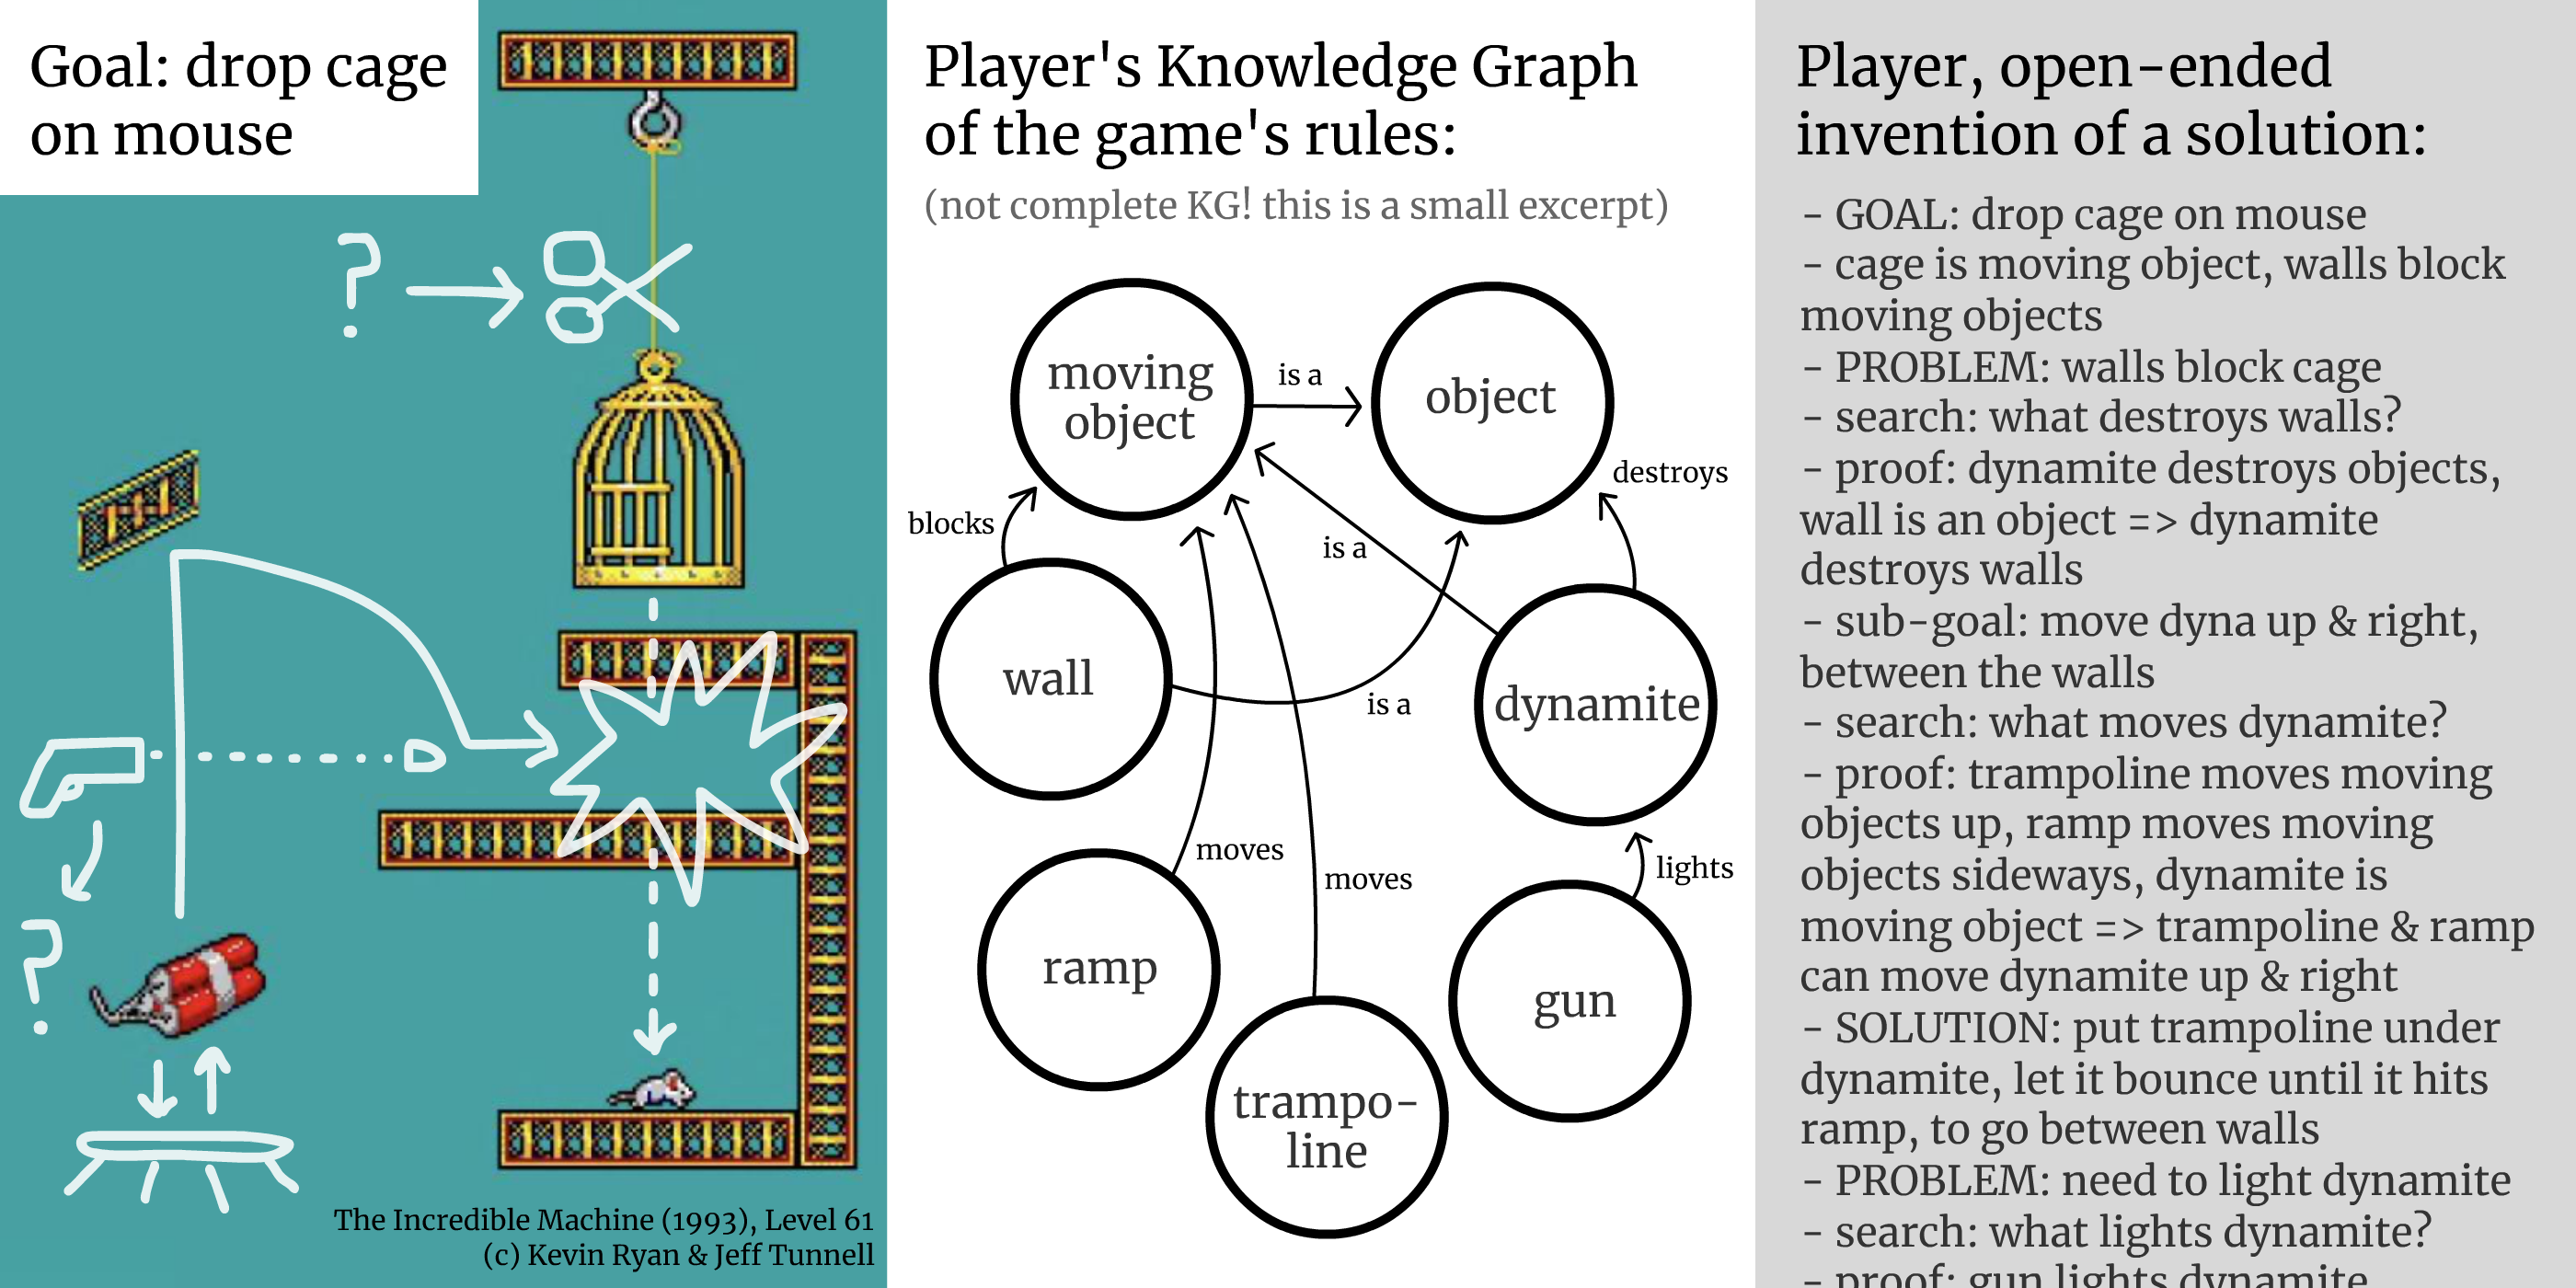
\includegraphics[width=\linewidth]{figures/across/tim.png}
    \caption{Example of how one could solve a game of open-ended innovation (above: \textit{The Incredible Machine}) via pathfinding through connected-idea space (a Knowledge Graph/Database).}
    \label{fig:the_incredible_machine}
\end{figure*}

From this, we can speculate they'll be akin to videogames featuring open-ended innovation (\autoref{fig:nostalgia}), like \textit{Lemmings} (1991), \textit{The Incredible Machine} (1993), \textit{Kerbal Space Program} (2015), \textit{Infinifactory} (2015), and other programming/engineering/design-inspired games. Common features of these kinds of games include:

\begin{itemize}
    \item \uline{Extremely wide search space}. The branching factor at each choice could be in the \textit{hundreds} (e.g. place what item, at what position, in what orientation) in contrast to Sokoban (branching factor 4) or even chess (branching factor $\sim$31).
    \item \uline{Requires an explicit causal model \& \textit{very} long-horizon planning}. e.g. in \textit{The Incredible Machine} and \textit{Infinifactory}, two machine-making games, you have to set everything up in advance, \textit{then} watch it play out, possibly up to a minute or more. An AI \textit{cannot} efficiently A* or SGD their way to a solution on this; you \textit{need} a causal model.
    \item \uline{Dense, almost all-to-all Knowledge Graph}. Every game mechanic interacts with almost every other game mechanic, leading to what designers call ``emergent gameplay'' \citep{juul_emergence}. The result: it's \textit{guaranteed} that players will find solutions that even the developers never imagined.
\end{itemize}

So, how do you search a space so vast, even \textit{its own developers} haven't fully explored it? In our previous section, \hyperref[sec:search]{Problem-Solving is Search}, we hypothesized that having an explicit Knowledge Graph/Database is \textit{crucial} for open-ended innovation, by pathfinding through connected-idea space. So, we suspect a good solver for ARC-AGI-4 \textit{must} build an explicit high-level symbolic knowledge base (whether or not it's KG format specifically). Earlier, we gave two discovery-fictions of how Diffusion Models and General Relativity could have been invented via KG search. In \autoref{fig:the_incredible_machine}, we offer one more example of how a KG search could solve a later hard level from \textit{The Incredible Machine} (1993), which — again, complete speculation — the ARC-AGI-4 ``open-ended innovation'' games may be inspired by.

\subsection{Coding Agent, Code Thyself (LLMs + DreamCoder + AlexNot)}
\begin{quote}
Everyone will not just. If your solution to some problem relies on “If everyone would just…” then you do not have a solution. Everyone is not going to just. At no time in the history of the universe has everyone just, and they’re not going to start now.

— @squareallworthy on Tumblr (2017)    
\end{quote}
The tech industry is not going to ``just'' rebuild AI on more rigorous, trustworthy foundations. Not when R\&D's results can be easily copied, the suits only think one financial quarter ahead, and big money is still flowing (for now). So if we want Neuro-Symbolic AI to go mainstream, and not stay restricted to preachy papers like this one (hi Gary), the designs have to be \textit{incentive-compatible}. Actually, stricter than that: they have to be \textit{gradient}-compatible: every step along the way needs to pay dividends quick, \textit{and} it has to use tools \& systems that developers already use. 

(As a recent success case in Neuro-Symbolic hybrids, consider the viral success of Jev \citep{jev}: a fast structured-output general text classifier, which lets you write normal code but call a small ``System 1'' AI as needed. The technical capability to make Jev existed years before Jev — it's `just' BERT \citep{bert} and zero-shot text classification \citep{zero_shot_nli} — but Jev spread fast because it was \textit{gradient}-compatible: easy to see/try/understand, easy to fit into existing workflows, instant dividends.\footnote{In particular, Jev did two things that made it hit Rogers's 5 Factors: 1) Pre-training it on a lot of general-domain data, so you can just plug it in, in contrast to having to collect data \& train your own BERT. And 2) Marketing/Design, like ``it can play Doom'', to make it easy to understand even for junior devs. (Though to be honest, some of their marketing was dishonest, e.g. ``it \textit{can't} hallucinate'' of \textit{course} it can, ask Jev “I need to wash my car. The car wash is 100 meters away. Should I walk or drive?” and it'll give the probability distribution 86\% Walk, 14\% Drive.)} See also: Rogers's factors for the diffusion of innovations \citep{rogers_diffusion}. We also bring up Jev to pre-empt a concern you may have of the following section: if it's such a good idea, why isn't it already done? We claim there's years-long ``overhang'' in the space of good ideas: Jev was technically possible for 7+ years since BERT, and what we're about to describe below was only practical starting about a year ago, with good-enough coding agents.) 

So, here's a design for a DreamCoder \citep{dreamcoder} + AlexNot-inspired loop, using LLMs as the `transition fuel' to give us cheaper, cleaner, trustworthy Neuro-Symbolic hybrids. For lack of a standard phrase in the literature, let's call the process of converting neural to neuro-symbolic \textbf{``cyborgification''}. If you can think of a less-terrible name, let us know.

First, note there's two kinds of knowledge \citep{ryle_concept_of_mind}: \textbf{procedural knowledge} (know-how) and \textbf{declarative knowledge} (know-what). Let's see each, in turn.

\begin{figure*}[b]
    \centering
    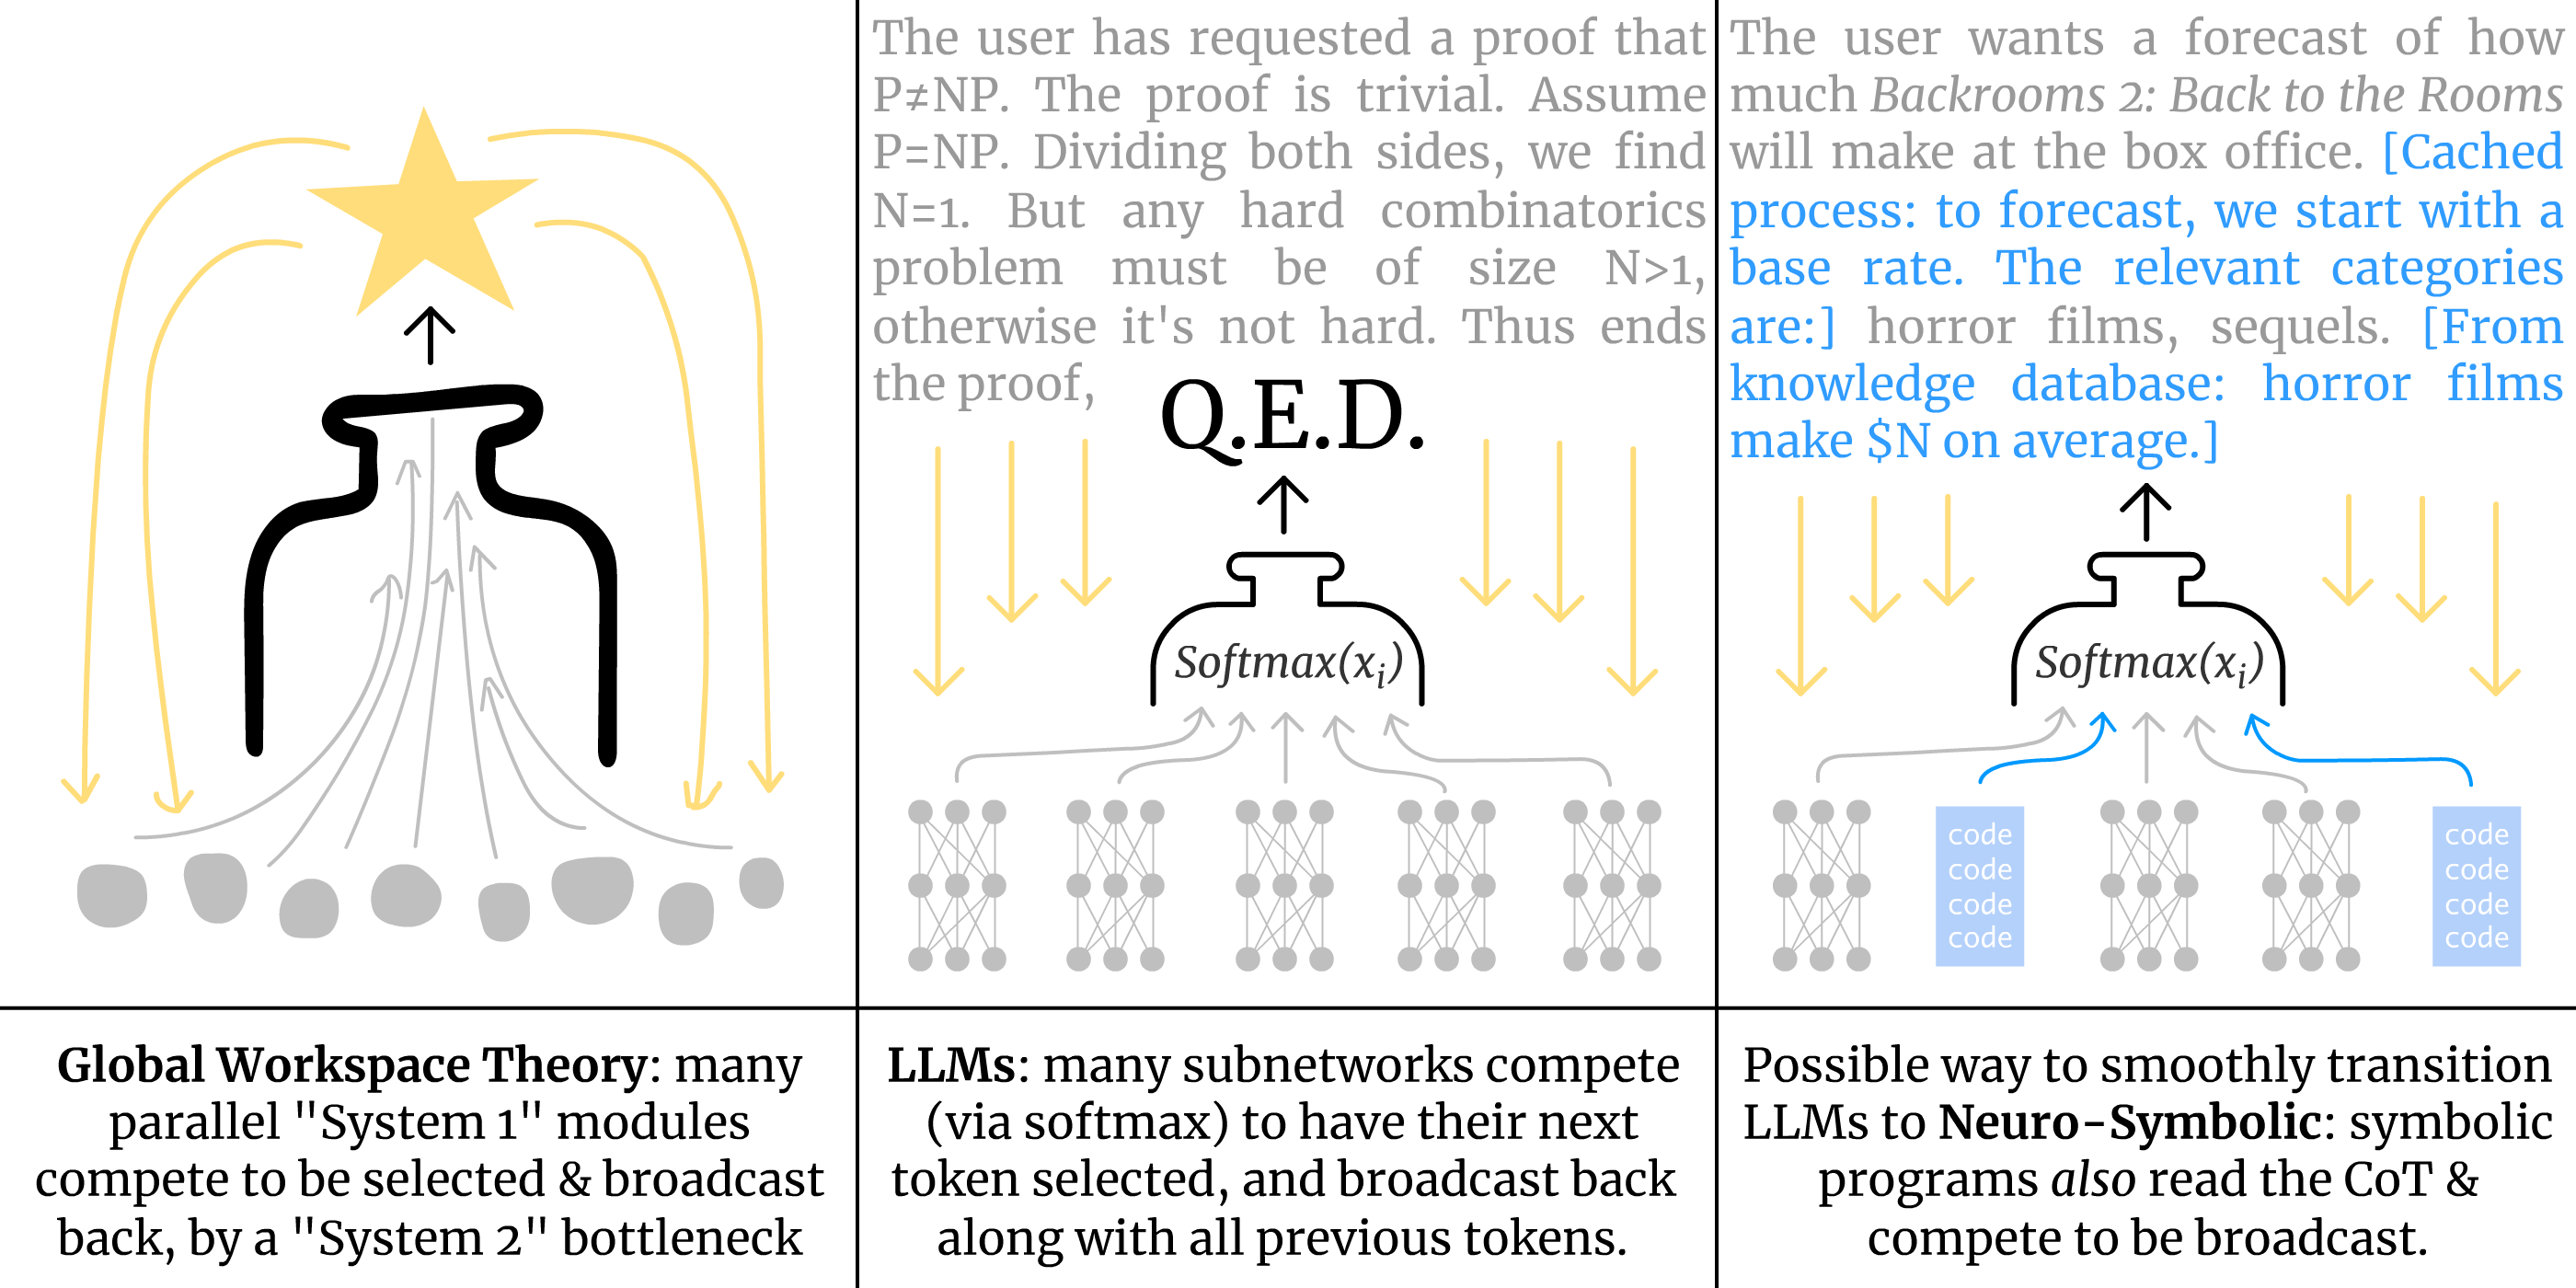
\includegraphics[width=\linewidth]{figures/across/cyborg_1.png}
    \caption{How Reasoning-LLMs are \textit{implicitly} similar to GWT, and how to make that \textit{explicit} with a Neuro-Symbolic hybrid.}
    \label{fig:gwt_transformer}
\end{figure*}

\textbf{Cyborgifying Know-How:}

As hinted in our earlier section, \hyperref[sec:search]{Problem-Solving is Search}, we can think of LLMs as indirectly implementing Global Workspace Theory: the Transformer is several sub-networks working in parallel, competing for the small softmax bottleneck, to have a token \& all previous tokens re-broadcast to all implicit parallel sub-networks, repeat. (See \autoref{fig:gwt_transformer}) And if an LLM has a Mixture-of-Experts architecture, then the parallel sub-networks are explicit.

But what if some of those Experts are \textit{just code}, maybe with some hooks into Jev-likes and other fast ``System 1'' classifiers? Moreover, what if these code-based Experts are written \textit{by the LLM itself?} (or a different `teacher' LLM?) Let's call these code-based Experts \textbf{``codelets''}, after \citet{copycat}. Like the neural experts, they read \textit{the same context} as input, but can output \textit{as many tokens as they want} in a single pass, along with a ``how important is this message'' score. The codelets' importance score goes into the same softmax function as the Transformer, letting \textit{both} neural and symbolic components use the same I/O: tokens in, token(s) with score out. Like a \textbf{``Unix philosophy for AGI''}: every codelet does one thing well, and they coordinate through the universal medium of text. 

Like regular LLM tools \& SKILL.md's, codelets can be plugged in and out between any LLM: great for the open-models community! But unlike tool calls, a codelet fires \textit{automatically} based on context: it doesn't have to rely on the LLM ``remembering'' to use that mental skill, it just \textit{does}. It's the difference between stopping to search Wikipedia, and just having Wikipedia directly installed in your brain.

Like regular Mixture-of-Experts, when to activate a codelet (its importance-score) can be learned, so they only batch-output tokens at the right time. But unlike regular Mixture-of-Experts, because codelets are \textit{just code}, an LLM coding agent can: a) do \textit{exact} credit assignment on the codelet's contribution, in contrast to backprop, by running the same task with the codelet on/off, b) edit the codelets instantly, no costly GPU re-training required, c) refactor codelets into a condensed, composable library with custom DSL (``library learning''), and d) make the codelets 100\% human-readable with comments, or even do automatic formal verification of the code, for safety/security guarantees.

\begin{figure*}[t]
    \centering
    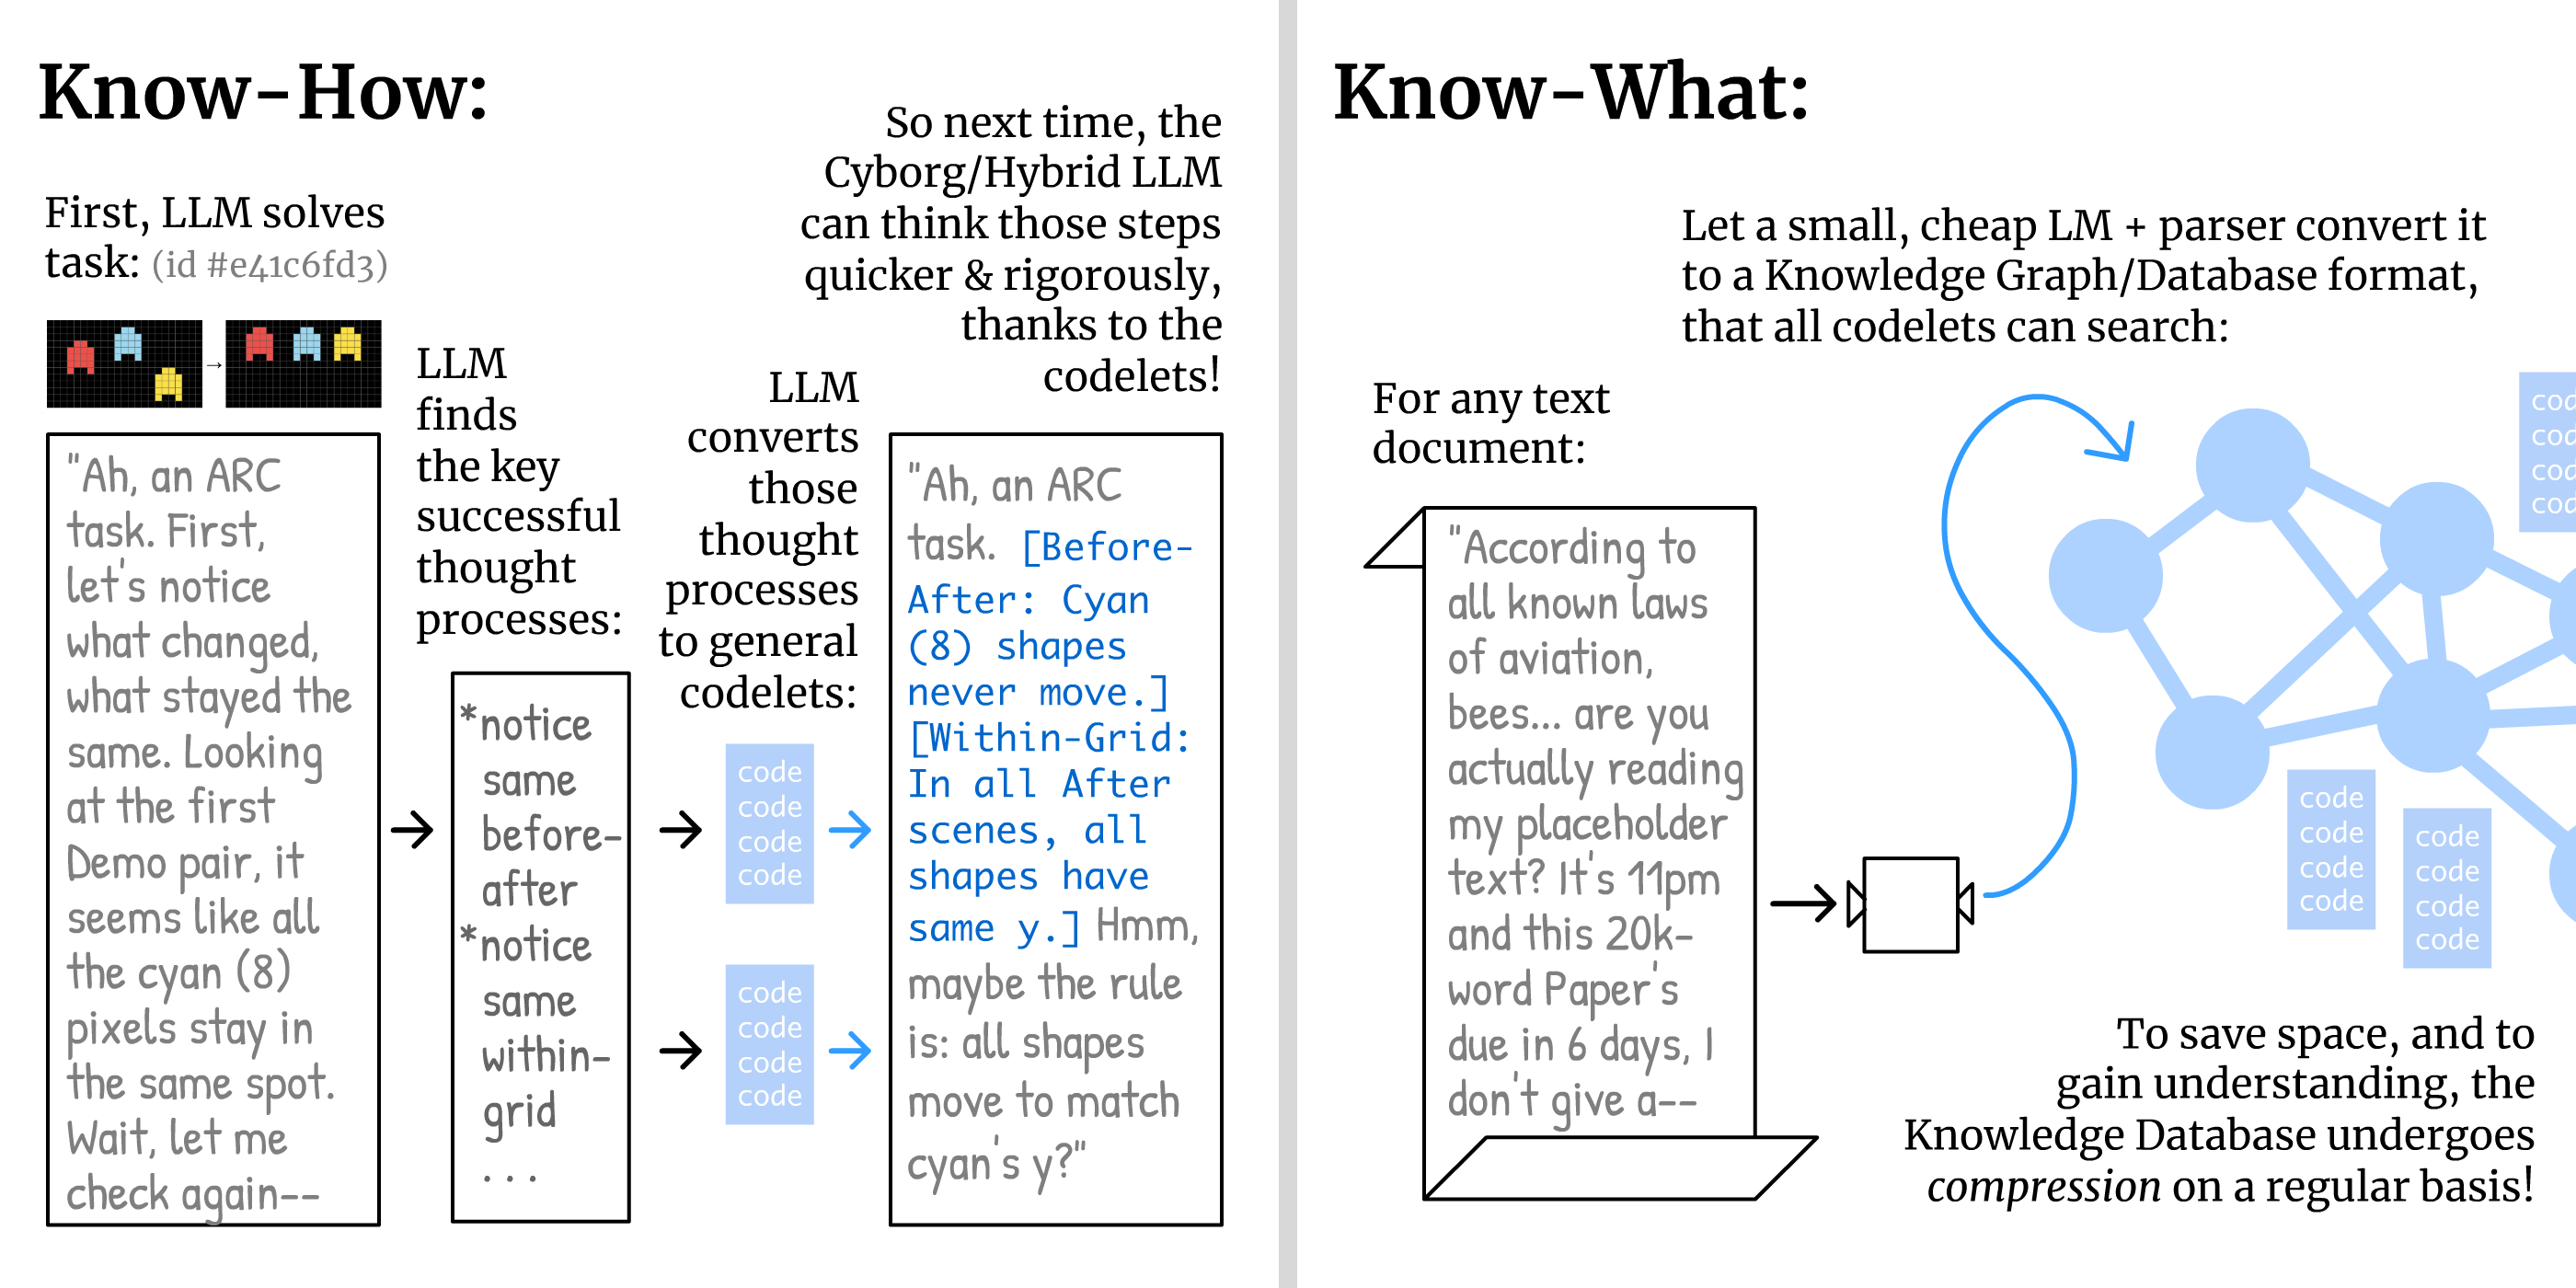
\includegraphics[width=\linewidth]{figures/across/cyborg_2.png}
    \caption{Design sketches of how to ``Cyborgify'' an LLM's procedural \& declarative knowledge.}
    \label{fig:cyborg}
\end{figure*}

Now, how to make an LLM cyborgify itself? (Or two separate LLMs: a `surgeon' agent cyborgifying a `patient' agent.) We can use a DreamCoder-style harness: during ``wake'', the AI solves problems, generating a Chain of Thought (CoT). During ``sleep'', the AI condenses parts of its CoT into When-Then pattern-matching codelets, AlexNot-style: programs that recognize When [pattern in context], Then [execute some program, output batched text + importance score]. Also during ``sleep'', the AI does AlexNot-style compression/condensation: select codelets for accuracy (usefulness on tasks) + simplicity + generalizability. (You could use a BERT/Jev-like/any text classifier to score the ``code smell'' on a codelet: will this code generalize? Is it nice \& modular, making it easy to re-use \& maintain? And so on.)

With an LLM coding agent re-coding itself, \textit{inference \uline{is} training.}

(Related prior work: DreamCoder \citep{dreamcoder}, obviously. For the old classics, see Blackboard architectures \citep{hearsay_blackboard} and Hofstadter's codelets \citep{copycat}. For more recent work that proves the general idea — LLMs significantly self-improving via self-made snippets later injected into its own CoT — see Metacognitive Reuse \citep{metacognitive_reuse}, Buffer of Thoughts \citep{buffer_of_thoughts}, and Dynamic Cheatsheet \citep{dynamic_cheatsheet}.)

\textbf{Cyborgifying Know-What:}

First, we need a language for storing any kind of symbolic knowledge. Traditionally, classic AI used \textbf{Knowledge Graphs (KG)} — facts in the form of triples, like: (Socrates, is a, man), (Man, is a, miserable pile of secrets), which lets you logically infer new facts, like: (Socrates, is a, miserable pile of secrets). But there's no need to stick to triples; arguably, \textit{trees} are the more natural unit of human thought: every taxonomy and physical scene graph is a tree, and we use syntax trees for natural language, computer programs, math equations, predicate logic, etc. It also doesn't have to be just text; the nodes of the trees could be images or sounds, for ``symbol grounding''. One last requirement, for Turing-completeness: our trees need to be able to point to themselves and each other. This lets us state \textit{facts about facts}, like assigning Bayesian uncertainty, fuzzy\footnote{Technical note: ``uncertainty'' $\neq$ ``fuzziness''. I'm uncertain if the trillionth digit of pi is even or odd, but it's not `fuzzy', it's definitely one or the other. Conversely: it's fuzzy what counts as upper atmosphere vs outer space, even if I'm 100\% certain exactly how many kilometres above sea level I am. Fuzzy truth values also help defuse paradoxes in self-referential statements. (see \citep{saving_truth_from_paradox}) ``This sentence is false'' just has fuzzy truth value $0.5$, whose negation is $1 - 0.5$, or still $0.5$.} truth values, and thinking critically about your sources — all requirements for trustworthy Scientist AI.

(See \autoref{fig:cyborg} for a general schematic of how to gradually cyborgify an LLM's know-how \& know-what.)

About now, you may be having spectral visions of \textsc{The Ghost of Cyc}. Early KG-based AIs like Cyc or IBM Watson were notoriously expensive, because humans had to manually convert knowledge to machine format. \textit{This problem is basically solved}, thanks to modern machine learning. (Google Knowledge Graph remains useful and profitable; KGs are currently used for real drug discovery \citep{baricitinib_kg}) It'd only cost a couple hundred bucks to run a small, specialized 1B model on 1,000 textbooks, to convert them to KG format. Transformers have also defeated the many problems that used to plague natural language processing, such as linking ambiguous pronouns\footnote{e.g. ``The trophy couldn't fit in the case because \textbf{it} was too \{big/small\}. What was too \{big/small\}?'' It used to be believed that AI solving Winograd problems like this would require it to have commonsense knowledge. Guess not.} (Winograd schema challenge) \citep{winograd_schema,winograd_defeat}

(And again, as real-world proof of the value of KGs: they're already helping with drug discovery \citep{kg_drug_discovery_review}, including the discovery of a Covid-19 treatment, which passed Phase 3 trials and got FDA emergency-approved \citep{baricitinib_kg,baricitinib_kg_method}.)

But we don't want just a collection of facts, we want \textit{understanding}. To do this, we get an AI to \textit{compress} the KG at regular intervals — during ``sleep''? — find regularities, factor them out, repeat. For example, it may recognize that \{pandemics, forest fires, communication network failures\} all involve \{things being connected, things being passed on through connections, tipping-point dynamics\}. From this, \textit{mere KG-compression} may generate the insight: they're all the same thing! This, in fact, is the core idea behind Percolation Theory.

Here's some immediate business benefits of offloading an LLM's knowledge, from its weights to a symbolic Knowledge Base:

\begin{enumerate}
    \item \uline{No hallucination}. Every fact has a source, and \textit{new} inferences from old facts can be formally verified. This no-hallucination guarantee is required in fields like law, finance, medicine, and safety-critical engineering. 
    \item \uline{No knowledge cutoff}. The \textit{day} research and news articles are published, you can convert them to KG format, and add them to the Knowledge Base, instantly usable by all models.
    \item \uline{No context rot/drift}. If all earlier context is also saved \& compressed to KG format, this would allow for continual learning, and robust long-horizon planning.
    \item \uline{Open-ended innovation}. If our hypothesis, ``open-ended problem-solving and -finding is just search through connected-idea space'', is true, then an explicit database of idea-connections could let LLMs make creative abductive ``jumps'' \citep{llms_cant_jump}. 
    \item \uline{You can easily delete information from an AI}, as easily as deleting entries from a database. This is good for privacy and security, but it's also good for AI \textit{capabilities}, since it lets us a) guarantee contamination-free benchmarking, and b) directly train AIs to beat Hassabis's ``Einstein Test'': \textit{could an AI, with knowledge only up to 1900, re-derive General Relativity?} And in general, we can start training \& backtesting AIs on the deepest scientific breakthroughs: given \textit{only} knowledge up to time T, re-derive as many discoveries as possible \textit{after} time T.\footnote{\citet{gpt1900} tried training an LLM on text prior to 1900, and found that while it mostly failed to regenerate 20th-century physics, when \textit{explicitly} given strange experimental observations, it could offer glimpses like “light is made up of definite quantities of energy”. See \citet{history_llms} for 4B LLMs trained on data up to 1913, 1929, 1933, 1939, 1946.}
\end{enumerate}

Ideally, we could even store \textit{know-how} programs and \textit{know-what} facts into the \textit{same} database; it's possible, both programs and natural language use syntax trees. This way, an AI simply \textit{reading} about a new mathematical method, would be instantly able to \textit{apply} it.

Honestly, we're kicking ourselves for only thinking of the above Neuro-Symbolic design sketch while finishing this paper, and not, like, 10 months ago. Oh well, there's always next year's ARC-AGI contest.

P.S: ...also while double-checking the citations for this paper, I just learnt that the inventor of Cyc, Douglas Lenat, died recently. Jeez, I hope my dunking on Cyc doesn't come off as too mean. One month before Lenat died, in his final co-authored paper \citep{lenat_marcus}, he proposed pretty much what we detailed above: LLMs to help generate a symbolic knowledge base, symbolic knowledge base to give rigorous power to LLMs. Maybe, after being laughed at for decades, Cyc \textit{will} have the last laugh after all. Rest in peace, Dr. Lenat.

\subsection{P2P AGI: a win-win-win for us all?}

It's a... controversial moment for our field. In the wake of the OpenAI–Hugging Face incident (and the German wiki incident (and the Australian Medicare incident (and that's just the ones we \textit{know} of))), our field faces a trilemma:

\begin{enumerate}
    \item Slow the progress of scientific research that could save lives, or
    \item Risk multi-billion-dollar cyber catastrophes or worse, or
    \item Concentrate power over AGI into a number of hands you could count on one hand.
\end{enumerate}

We argue (well, hope...) that \textbf{symbolic reasoning can cut the knot: it's a win-win-win for AI capabilities, AI security, \textit{and} fighting the concentration of power in AI!}

(Please note this is just one of many proposals for how to advance Safe AGI but in an open-source and people-empowering way. See also: Bengio’s Scientist AI \citep{bengio_scientist_ai}, Comprehensive AI Services \citep{drexler_cais}, Open Agency \citep{drexler_open_agency}, d/acc \citep{buterin_dacc}, Plurality \citep{plurality}, Civic AI \citep{civic_ai}, and AI 2040: Plan A \citep{ai_2040_plan_a}. Symbolic-first AI can complement, even enhance, all of these proposals. Also note that offering a technical solution does \textit{not} preclude policy changes, like protection of free speech for AI lab whistleblowers. Again, complement, not substitute.)

\textbf{AI Capabilities / Abundance:} As we showed with AlexNot and AlexNot-ODE, symbolic reasoning \textit{alone} can efficiently induce robust causal world models, even real-world scientific equations from noisy sparse data. And as we further argued in this paper, the strengths/weaknesses of the neural/symbolic approaches balance each other out, and LLMs can convert themselves — in a business-incentive-gradient-compatible way — into Neuro-Symbolic hybrids that are cheaper, hallucination-free, and better at open-ended innovation.

\textbf{AI Safety / Security:}
\begin{quote}
“You are not a God. You are simply \textit{bad product}.”

— The Boys, S3E4
\end{quote}
Many problems in AI Safety \citep{concrete_problems} are much easier to solve, if we make AIs that “think” primarily in symbolic world models (while using neural assistance for perception \& heuristics). For example:

\begin{itemize}
    \item \textbf{Interpretability} and \textbf{Eliciting Latent Knowledge} \citep{elk} become trivial. There \textit{is no} latent, hidden knowledge. You can just \textit{read} an AI’s world model. Even a layperson end-user could do this. This is vital for high-stakes fields like law, medicine, and civil engineering. As \citet{rudin_stop_explaining}'s excellent title bluntly puts it: ``Stop Explaining Black Box Machine Learning Models for High Stakes Decisions and Use Interpretable Models Instead''.
    \item \textbf{Faithful Chain of Thought, Formal verification:} LLMs’ out-loud ``thinking'' doesn’t always reflect their actual information-processing \citep{turpin_unfaithful_cot}. But a symbolic-first AI could get a cited source for every \textit{known} fact, and a formal logical proof for every \textit{new} inferred fact. \citet{tegmark_provably_safe} argues that formal verification is ``the only path to controllable AGI''; we're not \textit{that} pessimistic, but we agree formal proof is the best guarantee, so if we \textit{can} do it, why not?
    \item \textbf{Unlearning:} Want to ship an AI you trained indiscriminately on the whole internet, but \textit{not} ship dangerous bioweapons knowledge, or doxx individuals’ private info? With LLMs, it’s easy to override refusal \citep{gcg_attack,refusal_direction}, and hard to delete latent knowledge \citep{lucki_unlearning}. But with a Knowledge Database, it’s trivial: just search \& delete those entries.
    \item \textbf{Non-agentic Tool AIs:} AlexNot-ODE is a proof of concept that a symbolic-first AI \textit{can} do useful scientific work, \textit{without} being agentic. A non-agentic tool AI can’t “go rogue” any more than a toaster can. (See also: \citet{bengio_scientist_ai}'s proposal for non-agentic `Scientist AI'.)
    \item \textbf{Robustness:} You don’t want your “shop for me” agent to read a jailbreak that tricks it into buying 1,000 individually-wrapped beans. Neural networks are prone to adversarial inputs, out-of-distribution failure, and confusing correlation for causation. But a symbolic-first AI, with formal verification built into its loop, \textit{can’t} be tricked, any more than you can “jailbreak” a calculator into telling you 2+2=5.
    \item \textbf{Learning human values:} Related to “robustness”, much of LLMs’ success is due to RLHF \citep{rlhf,instructgpt}, which lets them learn what humans value. But like all neural learning, it’s fragile: LLMs learn to be sycophantic \citep{sycophancy}, or more annoyingly, give nonsense “pushback” to pass tests for sycophancy. But an AI that induces Bayesian causal models for \textit{everything} — including human values — could \textit{actually understand} what causes human flourishing. \citep{inverse_rl,cirl}
\end{itemize}

AI Security/Safety isn’t “just” about preventing catastrophic loss-of-control scenarios. It’s also good business: why would you \textit{want} to rent an AI that might unpredictably execute state-level cyberattacks on your own company? That is not a God, that is simply \textit{bad product}.

\begin{figure*}[t]
    \centering
    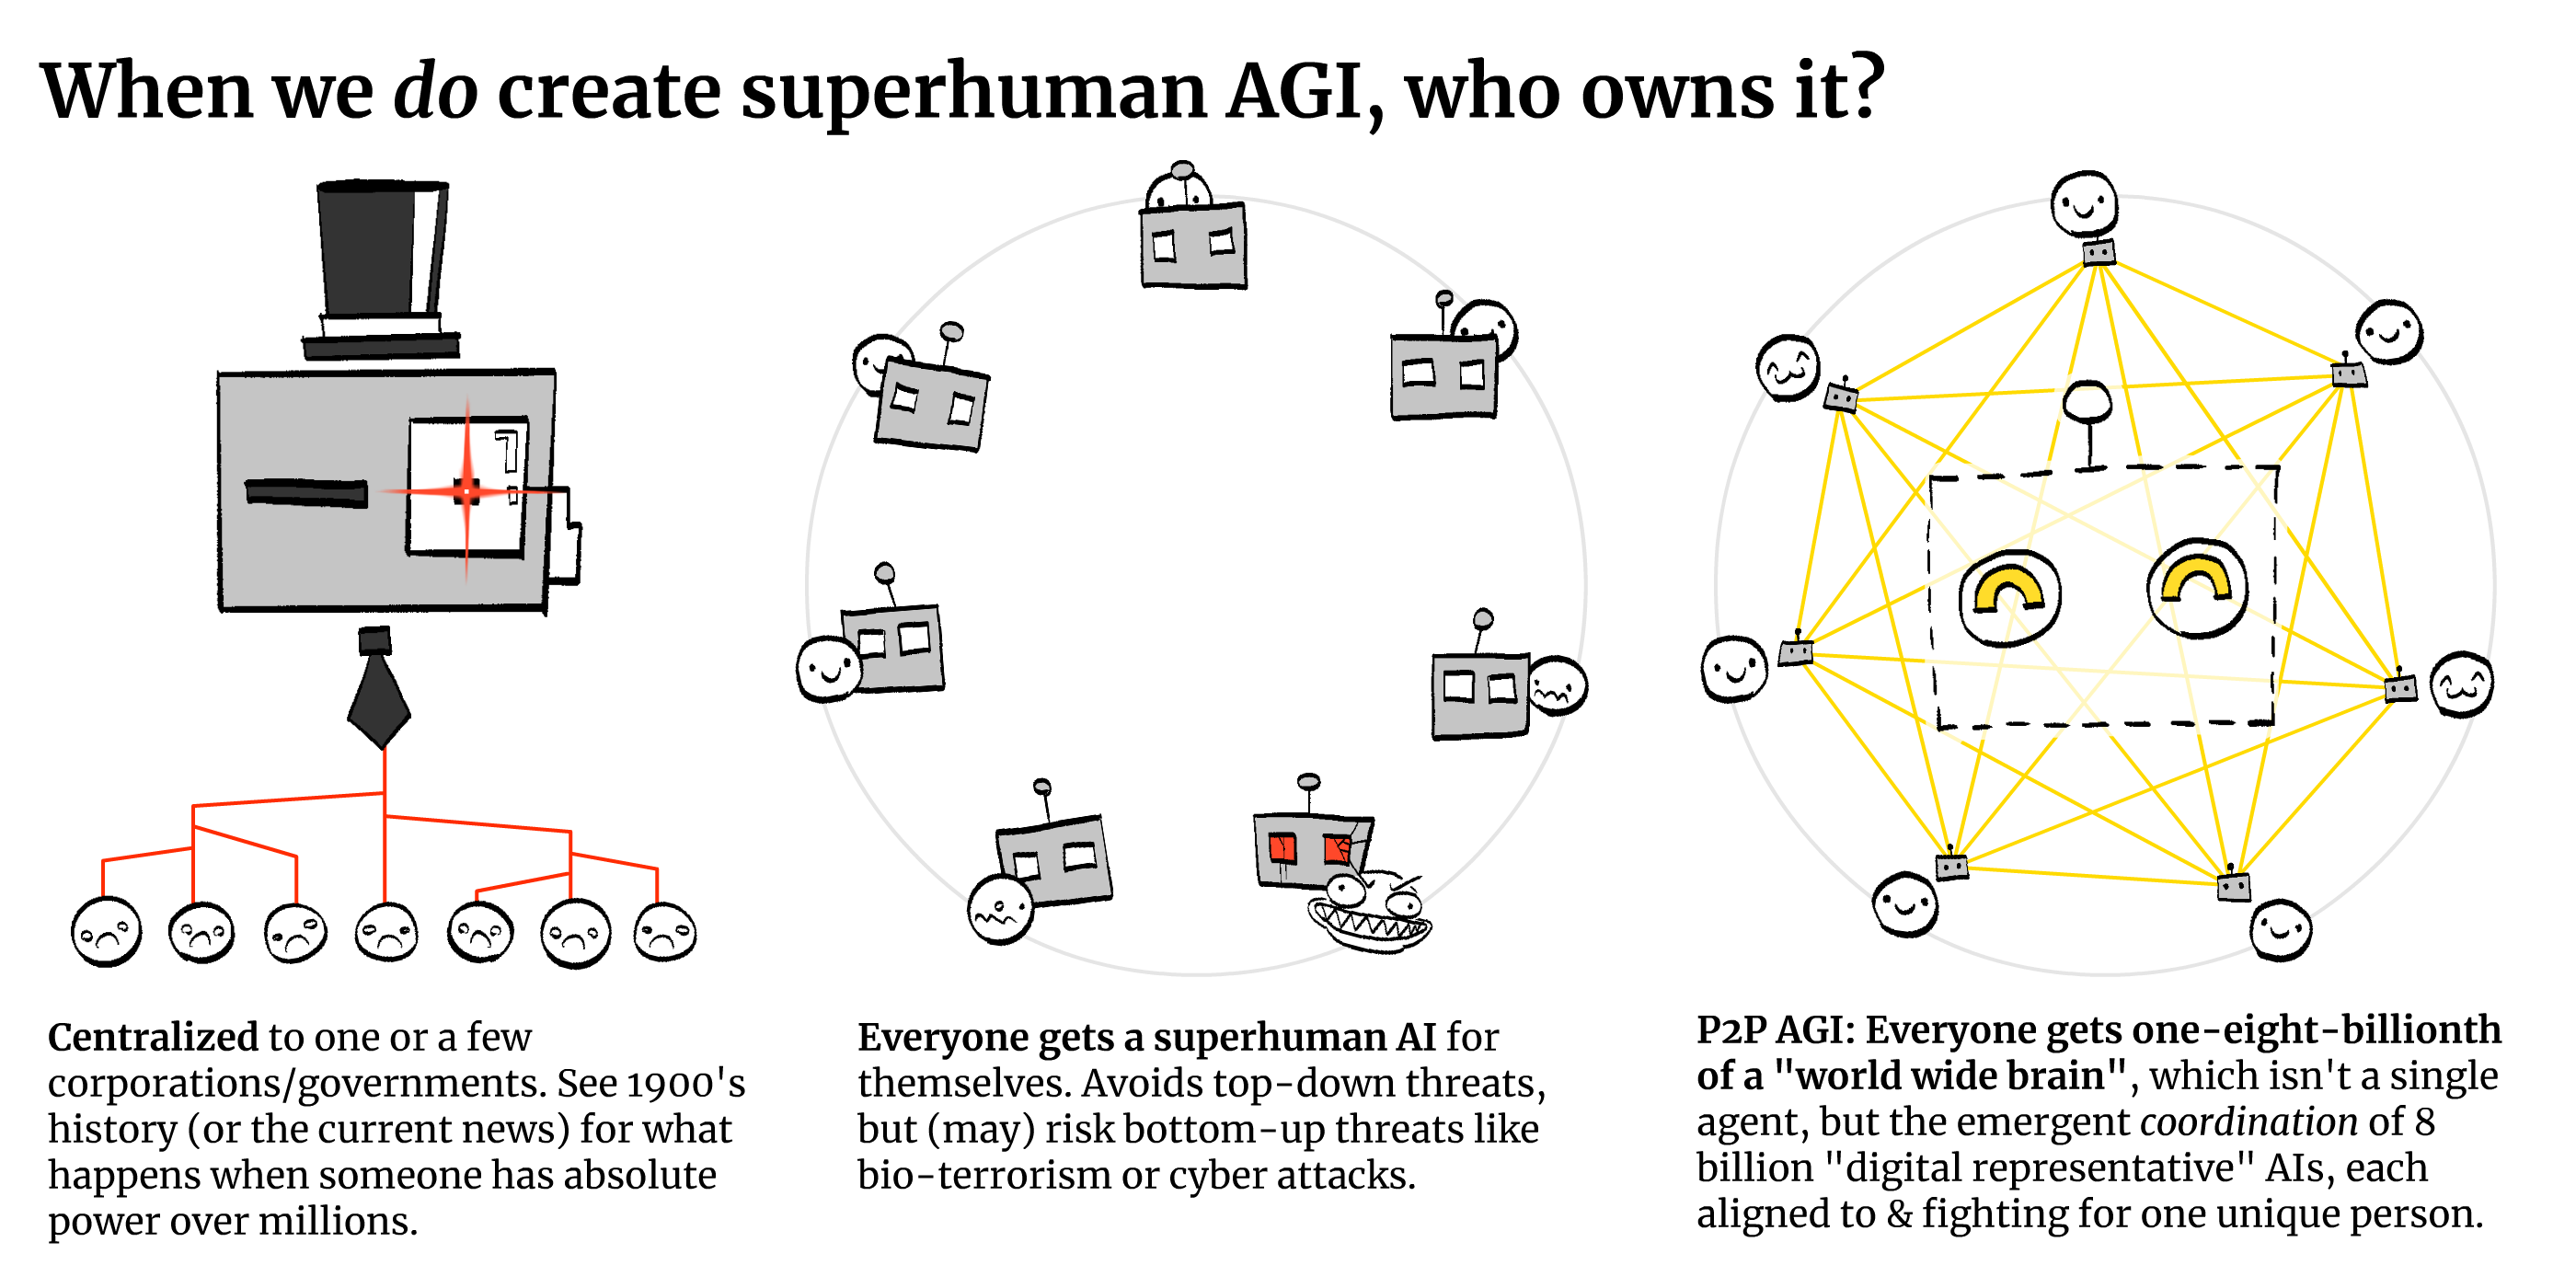
\includegraphics[width=\linewidth]{figures/across/p2p_agi.png}
    \caption{Who owns AGI?}
    \label{fig:p2p_agi}
\end{figure*}

\textbf{Decentralizing AI:}

CEOs: “AGI will help us cure cancer!”

Everyone Else: “Yeah, \textit{for you}. For us, you’ll make the cure cost a zillion dollars, like you did with insulin.”

The AI X-Risk people worry about deceptively-aligned power-seeking AGI ruling the world, and causing human extinction. Whether or not they're right, we should \textit{also} worry about AGI aligned to the deceptive power-seeking \textit{humans} who already rule the world: a cybernetic boot stamping on a human face, forever, would be a fate \textit{worse} than extinction \citep{malevolent_actors_80k}. So any solution to AGI Risk should \textit{not} increase AGI power concentration. And when our field finally invents AGI, it must empower \textit{people}, not just the already-powerful.

Democratizing AI may protect against top-down totalitarian threats, but what about bottom-up terrorist threats, e.g. people using open-source AI for cyberattacks on hospitals? To mitigate this, we propose \textbf{Peer-To-Peer AGI}: not \textit{one} superintelligence in the hands of one corporation/government, nor all 8 billion people getting their own personal superintelligence, but \textbf{everyone getting a one-8-billionth slice of a World Wide Brain} (\autoref{fig:p2p_agi}), that emerges from the coordination of 8 billion smaller AI agents, each one aligned to their unique human. (To guarantee one-agent-per-human for democratic decisions in a privacy-preserving way, we could use Zero-Knowledge ID proofs \citep{camenisch_anonymous_credentials,semaphore}. It \textit{may} also eventually be safe to give each person their own superintelligence, as long as the humanity-aligned World Wide Brain stays 8 billion steps ahead.)

\textbf{Why P2P:} Well-designed peer-to-peer protocols allow for \textit{coordination without centralization}. This way, we can solve global problems, without putting the corrupting nature of power into any one group of people. A good P2P protocol should also be defence-favouring, and robust to defectors: if 0.1\% of people want to make an omnicidal bioweapon, they’d only get 0.1\% of The Brain, vs the other 99.9\% of The Brain that’s dedicated to stopping them. But a well-designed P2P AGI shouldn’t be a naïve tyranny of the majority; it should strive to find the best win-win social contracts for all. See: Pol.is, Community Notes \& other bridging-based algorithms \citep{tang_alignment_top_down}.

\textbf{Why coordination:} While it's clear how AGI can help us with problems bottlenecked by science (e.g. curing Alzheimer's), what about problems bottlenecked by \textit{humans?} (e.g. the cost-of-living crisis.) To illustrate how P2P AGI can help, consider lobbying. In 2025, US lobbyists spent \$5.13 billion in total \citep{opensecrets_lobbying}. That's a lot, but with 270 million American adults, that's \textit{less than \$2 a month} per American adult. For comparison, the average American spends over 10$\times$ that amount on \textit{candy} \citep{nca_candy_2024}. However, it's the classic diffuse-vs-concentrated-interests problem \citep{olson_collective_action}: it's much easier for three CEOs to coordinate against us, than 270 million adults coordinating to fight back.\footnote{This example is America-centric, but the lobbying-per-citizen numbers are similar to other developed nations, and the same arguments apply.}

\textit{But P2P AGI could bring the cost of coordination to zero.} Imagine: everyone has a local, open-source AI Agent on their phone, aligned not to some corporation, but to \textit{you}, \textit{your} individual dreams and hopes. The Agent helps you with day-to-day tasks, helps you live according to your values, when one day they pop up and ask: ``Hey, for the price of a Netflix subscription, would you like to end the cost-of-living crisis, pharma price-jacking, and fight every lobbyist? Me and the other 270 million American Agents talked last night. We're doing a Kickstarter-style coordination mechanism: if-and-only-if 80\%+ of you agree to this, then we'll take \$19.99/month each, to pool together \$50 billion — which is an order of magnitude more than \textit{all} US lobbying combined — and use it to save your country. And \textit{you personally} will have a day-to-day say in how this democratic fund is spent. Just talk to me, and I'll talk to my 270 million colleagues. Sound good?''\footnote{The Agents need not be conversational chatbots or person-shaped, they can ``just'' be Tool AIs. Also, they wouldn't literally do all-to-all communication, that scales terribly, but they could use any other proven P2P coordination protocol.}

``P2P AGI democracy'' sounds radical, but it's just the logical conclusion of \textit{every} part of the political spectrum:\footnote{Horseshoe Theory but Lawful Good?}

\begin{itemize}
    \item For moderates, it's just representative democracy, but with \textit{one representative per citizen}. You can \textit{personally talk} to your representative every day, and a formally-verified AI representative \textit{can't} lie or break promises, any more than a calculator can claim 1+1=3. Your AI representative would also understand basic science, history, and economics, which is more than I can say for our current human representatives.
    \item For leftists, it's ``Peer-to-Peer Cybersyn'': the dream of intelligently aligning an economy to the people, but because it's peer-to-peer, it can't be ended by a CIA-backed coup.
    \item For libertarians \& economic conservatives, it's ``Coasean Bargaining at Scale'' \citep{krier_coasean}: a market with \textit{zero} bargaining costs would resolve market failures on its own: it can self-correct on pollution, fund public science \& defence, and so on.
\end{itemize}

\textbf{Open-source gets an unfair advantage:} Open-\textit{weight} models are great, don't get us wrong. But while they democratize AI \textit{inference}, they don't democratize AI \textit{training}. But if we used (something like) the ``Cyborg'' design sketched above, where \textit{inference \uline{is} training} — an LLM coding agent on a laptop could make new codelets and KGs to share with \textit{every} Agent, since they all use a common ``Unix Philosophy for AGI'' design — then AI \textit{training} can also belong to the people.

As an illustration of how powerful citizen-computation can be: during the Covid-19 pandemic, the citizen-science project Folding@home (which let folks run protein-folding simulations on their own personal computers) got more volunteer compute than \textit{the top 500 supercomputers combined} \citep{folding_at_home}. Now imagine a citizen-owned P2P AGI with more compute than the top AI labs combined, that doesn't just \textit{run} projects like Folding@home, it can \textit{create} projects like Folding@home — by inducing robust symbolic models from sparse noisy data — for \textit{every} area of science.

. . .

Back to reality. The above fantasy — and it \textit{is} fantasy, for now — requires that AI:

\begin{itemize}
    \item Can accurately learn \& be aligned to \textit{one} human user's values.
    \item Can do multi-agent coordination, \textit{aligned to their human users}.
    \item Can do robust, hallucination-free, long-horizon planning.
    \item Can be formally verified, and interpreted by \textit{laypeople end-users}.
    \item Can be run \textit{locally on a phone}, and trained in a P2P way across millions of consumer devices.
\end{itemize}

We argue (hope) that \textit{symbolic-first AI} can accelerate all 5 of the above requirements. Perhaps a ``Unix Philosophy for P2P AGI'', with LLMs cyborgifying themselves with open-source codelets \& KGs, through a DreamCoder+AlexNot-style harness — or something else entirely. As we showed in this paper, symbolic reasoning \textit{can} unlock robust causal world modelling, while being 100\% interpretable and verifiable, all at extreme time/cost/data-efficiency on already-democratized hardware.

We know this is really lofty for a paper about an AI that scored 13\% on a gridworld task, but hey, Ada Lovelace programmed a computer that didn't even exist, and she dreamed of machines composing stunning works of music \citep{lovelace_notes}. We dream of a future where Neuro-Symbolic AI can reason flexibly-yet-rigorously, with full transparency \& provable alignment to humane values, to give rise to a trustworthy Peer-to-Peer AGI that belongs to \textit{everyone}.

That's a future worth building.











%%%%%%%%%%%%%%%%%%%%%%%%%%%%%%%%%%%%%%%%%%%%%%%%%%%%%%%%%%%%%%%%%%%%%%%%%%%%%%%%%%%%%%
%%%%%%%%%%%%%%%%%%%%%%%%%%%%%%%%%%%%%%%%%%%%%%%%%%%%%%%%%%%%%%%%%%%%%%%%%%%%%%%%%%%%%%
% CONCLUSION 
%%%%%%%%%%%%%%%%%%%%%%%%%%%%%%%%%%%%%%%%%%%%%%%%%%%%%%%%%%%%%%%%%%%%%%%%%%%%%%%%%%%%%%
%%%%%%%%%%%%%%%%%%%%%%%%%%%%%%%%%%%%%%%%%%%%%%%%%%%%%%%%%%%%%%%%%%%%%%%%%%%%%%%%%%%%%%

\section{Conclusion: The Sweet Lesson of Actually Understanding Stuff}\label{sec:conclusion}

Imagine BubbleSort was invented, but not QuickSort. Theoreticians warn that BubbleSort is inefficient in $O(n^2)$, and there \textit{must} be a better way in $O(n \log n)$. Meanwhile, industry rolls their eyes and retorts, ``lol Moore's Law goes brrrr'' — and it \textit{does}. BubbleSort may be inefficient, but you can disguise the stink with exponential resources. From the outside, it looks like the theorycels were wrong: BubbleSort never ``hits a wall'', bigger \& bigger lists get sorted in less \& less time. But in a way, this silent failure is \textit{worse} than a loud wall: it tricks us into complacency, scaling up a wasteful idea.

We claim that modern deep learning is in this situation. Theoreticians warn how inefficient LLMs are: human brains need $\sim$10,000$\times$ less linguistic data than LLMs to gain the same level of fluency \citep{frank_data_gap}. And we \textit{empirically} see exponential inefficiency: each frontier model costs 10$\times$ more money to train, and performance scales logarithmically with CoT length \& swarm agents \citep{ord_scaling_paradox,ord_log_x_chart,ord_swarm_scaling}. However, you can disguise the stink with \textit{two} exponential inputs: Moore's Law, and VC money. Throw 2 exponential resources into 1 exponential inefficiency, and AI \textit{will} improve exponentially... for now. There's a race to the bottom on token prices, free open-weight models only lag a few months behind paid ones \citep{epoch_open_closed_gap}, and hyperscaler capex already outstrips operating cash flow \citep{tikr_capex_gap}. Given all this, the AI industry may run out of cash before reaching AGI.

\textit{Unless:} starting right now, we use LLMs as a `transition fuel' to create cleaner, more-efficient AI — like how coal gave us the industrial capacity to replace coal.

Rich Sutton's \textit{The Bitter Lesson} \citep{bitter_lesson} is one of the most misinterpreted essays on modern AI. In the popular misconception, people round it off to ``lol scaling goes brrr''. But as Sutton himself has clarified several times since, his point was that \textbf{we need simple architectures that scale, not that \textit{any} simple architecture will scale.} ``Simple'' ideas still need to be invented. Deep Blue didn't scale to Go: we had to (re)invent neural networks. Plain neural networks didn't scale to advanced language modelling: we had to invent Transformers. And now, Sutton \citep{sutton_dwarkesh} himself has warned that Transformer-based LLMs won't scale to AGI: we need to invent...

...well, we don't know yet. But we hope this paper can be evidence for \textit{The Sweet Lesson: theory pays off!} The classic principles of cognitive science \textit{work.} Understanding is compression/condensation, Problem-solving \& -finding is search, Intuition is pattern-matching. We suspect `true' AGI will be a simple architecture based on these principles, merging System 1 \& 2 by merging neural \& symbolic. We further suspect there's business-incentive-gradient-compatible ways for LLMs to convert themselves to trustworthy Neuro-Symbolic hybrids, to give rise to an open-source, humanity-aligned, Peer-to-Peer AGI.

Finally, we hope we've exorcised \textsc{The Ghost of Cyc}, and convinced you: \textit{symbolic reasoning is cool again!} It can induce robust causal world models in novel scenarios, is 100\% interpretable and verifiable, hyper-efficient in terms of cost/time/data, and fights the concentration of power in AI by running on already-democratized hardware. If LLMs are the coal of AI, Neuro-Symbolic could be the \textit{solar} of AI: cheaper, cleaner, decentralized, locally ownable by regular folks, \textit{and} creates massive abundance.

In sum: let's revisit the fundamentals of intelligence.

Let's \textit{understand understanding.}

\begin{figure*}[b]
    \centering
    
\includegraphics[width=\linewidth]{figures/across/FIN.png}
    \caption{Compress No Evil, Search No Evil, Pattern-Match No Evil}
    \label{fig:fin}
\end{figure*}


%%%%%%%%%%%%%%%%%%%%%%%%%%%%%%%%%%%%%%%%%%%%%%%
% CREDITS %%%%%%%%%%%%%%%%%%%%%%%%%%%%%%%%%%%%%
%%%%%%%%%%%%%%%%%%%%%%%%%%%%%%%%%%%%%%%%%%%%%%%

\section{Acknowledgements}

\textbf{Thank you to the ARC Prize Foundation} for running this contest, and making an AI benchmark that's actually grounded in cognitive science. We look forward to playing the ARC-AGI-4 games you cook up!

\textbf{AI Collaboration:} All main text in this paper was human\footnote{Well, a featherless biped, anyway.}-generated, test any section on Pangram.com if you don't believe us. (Yes, even the em dashes. You can pry the em dash — the superior punctuation mark — from my cold, human hands.) All illustrations were also human-generated. However, the Claude family of models assisted with research, finicky \LaTeX, data visualization figures, and fixing \sout{tpyos} typos. Claude also helped immensely with programming, because at this point, coding without LLMs is like driving without GPS. Everybody say Thank You Claude. (in unison: ``Thank You Claude'')

\textbf{Crowdfunding:} Nicky Case also gives her deepest gratitude to her Patreon/Ko-Fi supporters, for sticking with her for a year while she kept vagueposting, ``I'm doing a symbolic AI research thing, please hold''. I hope the wait was worth it! Supporter Name Credits are in Appendix~\ref{app:supporters}. Thank you! <3



%%%%%%%%%%%%%%%%%%%%%%%%%%%%%%%%%%%%%%%%%%%%%%%
% THE END %%%%%%%%%%%%%%%%%%%%%%%%%%%%%%%%%%%%%
%%%%%%%%%%%%%%%%%%%%%%%%%%%%%%%%%%%%%%%%%%%%%%%

% Less Crammed Biblo

\clearpage
\raggedbottom 
\onecolumn
\renewcommand{\bibfont}{\small\raggedright}
\setlength{\bibsep}{0.4em}        % less space between references
\begin{spacing}{1.0}
\bibliography{references/1_intro,references/1_intro_new,references/2_overview,references/3_compression,references/2_overview_new,references/3_compression_new,references/4_search,references/5_pattern_matching,references/6_results,references/7_future,references/8_conclusion}
\end{spacing}

% Appendix: Supporter Credits!

\appendix
\section{Supporter Credits <3}
\label{app:supporters}

\noindent This indie research was made possible by the support of the folks below. Thank y'all! (\href{https://patreon.com/ncase}{patreon}, \href{https://ko-fi.com/nickycase}{ko-fi})

\vspace{1.5em}

{\footnotesize\setstretch{0.85}\setlength{\parskip}{0.6em}  % tight lines within a name, more space between names
\begin{multicols}{7}\centering

3Blue1Brown \par Aatish Bhatia \par adam \par Adam Zeiner \par Aeryn Light \par Agent Entity \par Aidan H \par AkitoInoue \par al \par Alan Kay \par Alastair JL \par Albatross Ascot \par Ale G \par Alex Alperin \par Alex Be \par Alex Mitchell \par Alex Sanchez \par Alexander230 \par Amir Livne Bar-on \par AnAwesome Dudette \par Andrea Chlebikova \par Andrew \par Andrew J Hutzel \par Andy \par Anne Cummings \par Anthony Chivetta \par Antoine Genesi \par Antonio Checa \par Argzero \par Aria Minaei \par Artiom Casapu \par Aschelon \par Axolator \par Aygox \par Azerrr \par B Cavello \par Bas den Uijl \par Bastien \par Ben Kraft \par Ben Kravitz \par ben t \par Ben Walker \par Benoit Doidic \par Bo \par Bram Borger-Johnson \par Brandon Quinn \par Brendan Barnwell \par Brendan Nelligan \par Brian Ball \par Brian Cloutier \par Brian Lange \par Brian Moore \par Brian Wu \par Bruce \par Brume \par BuckleStitch \par Burkhard \par Cary Huang \par Cat Manning \par Catherine J Smith \par Cedric Nering \par Celery Farm \par CERN Doughnut \par Chen Li \par Chloe Lehnert \par Chris Ferrie \par Chris Hallacy \par Chris Lam \par Chris Makler \par Chris Ploeg \par Christopher Bradley \par CmdEngineer \par cmotuz . \par Colin \par Colin Liotta \par ColorfulCast \par Colton Neves \par Comm Luke \par Connor Harrison \par Cort Stratton \par Coyote Codornices Marin \par Craig Eby \par Cristy Stone \par Da LIberman \par dan cooney \par Dan Schroeder \par Dan Wahl \par Daniel Hires \par Daniele \par Danielle Strachman \par Danni \par Darius Bacon \par Darrin Massena \par Dasein Wave \par daudiihhdau \par Dave Tu \par David Garwin \par David Hayes \par David Mora \par Dimitri \par Dión \par Djadj0u \par Dominic Scott \par Dominik Gabl \par Don Kimber \par Dubek \par Ducks \par Dvir Moran \par Dylan Meconis \par Dylan Wootton \par E Drake Kajioka \par Eddie \par Edward Jones \par Eleanor \par Elizabeth Ann Ditz \par Emelin Ringuette \par Emerson Ford \par Emily Hunter \par Empireman \par Eric Bell \par Eric Chisholm \par Eric Willisson \par Erin Ingram \par Ethan Mollick \par Ethar Alali \par Eugene Eric Kim \par Evan Broder \par Evan Rocha \par Evan Shulman \par Everett Wetchler \par Fahrstuhl \par Fain \par Fanboat \par Fey Technologist \par Fiona Nielsen \par Flote37 \par Frank Leon Rose \par FreNeS1 \par FXuanzi C \par Gaëtan Perrault \par Geoffrey Litt \par George Woodliff-Stanley \par Gerrit Essmann \par getabyte1432 \par Gevroska \par Giacomo Pareschi \par GiovanH \par Glenn Willen \par griotspeak \par guguke \par Gui Ambros \par gunduzc \par Hakase \par Harry Brisson \par Hed Bar-Nissan \par Henry Reich \par Henry Swanson \par Herbert Schilling \par HI \par Hilary Fried \par Hsien-Chih Chang \par Husakov \par Ian K \par informal dehyde \par irina \par Isa Marin \par Isaac \par ItsMeMaxine \par Ivan Carlestam \par Ivo Murrell \par Jace \par Jacques Frechet \par James \par James Babcock \par JAMES HORTON \par James Zaki \par James Zhu \par Jamie Wong \par Jan Cho \par Jay Zuerndorfer \par Jayden Campbell \par Jeanne Kramer-Smyth \par Jeff \par Jeffery Olson \par Jennifer \par Jeroen Koomen \par Jesper \par Jesper the End \par Jesse \par Jesse Bradley-Amore \par Jim Meyer \par Joe Carroll \par Joe Marasco \par Joe Mou \par Joe Sevits \par John H \par John Leonard \par John Stout \par John\_Ca \par Jonathan Ng \par Jose Varela \par Josh \par Josh Delgado42 \par Joyce Ng \par julian plaga \par Julianne Hammink \par Julien Calixte \par Justin Clark \par Juukii \par kaigani turner \par Kailys \par Kalu \par Karen Haldrup Lund Jakobsen \par Karl Niu \par Kat \par kate \par Katie Harvey \par Katie Worth \par Katinka \par Kay \par Kayla \par Kayle \par Kelly Grantham \par KendallZhu \par Kendra Lockman \par Kent Shikama \par Kevin \par Kevin Zollman \par Kim Viens \par klimpner \par KM \par Koen \par kOrc \par Krakenova \par Krayt \par Kris Noble \par Kristján \par Lev \par Lev R \par Lexi \par Lily W \par Lisa Hemphill \par louije \par lucafeu \par Lucas Garron \par Luke FitzSimons \par Lyrandar \par M \par Malcolm Ocean \par Malex \par Manual Cookie \par Marcus Phillips \par Marie Friberger \par Mark Guzdial \par Marlaine Olinick \par Martin Schneider \par Mary \par Mats Borges \par Matt Hughes \par Matt Payne \par Matt Rogers \par Matt Wang \par Matthew Cook \par Mauricio Arreola-Garcia \par Maxim \par Maximilian Beier \par Maya Tung \par Meeni Levi \par Mega Toadmaster \par Melon \par Merchant Of Soul \par Mercury Legba \par Merilee D. Karr \par Micah Cowan \par Michał Bartoszkiewicz \par Michael Forrest \par Michael Handler \par Michael LaCroix \par Michael LaHood \par Michael Lewis \par Michelangelo Grigni \par Michelle King \par Miguel Massaro \par Miguel Puche-Alonso \par Mikayla Hutchinson \par Mike Gifford \par Mike Pavlov \par Mikey \par Miki \par Milica Vlajkovic \par Mir \par miscmike \par Mitchell Wand \par Molly Jameson \par Moritz Stefaner \par Moshe Gordon Radian \par MZ \par NapuNawa \par Nat Kale \par Natalia Babaeva \par Nathan Borson \par Nathan Daly \par Neal McBurnett \par Neeldhara Misra \par NefariousToast \par Neil Halloran \par Nel Nuss \par Neren79 \par Nicolas \par Nicorov Spazin \par Nikita Vasilyev \par Nikolai Kruglikov \par Nirmal Mehta \par no \par Ntimi Schnütgen \par Nuno Delicado \par Olive Perry \par Olivia Brode-Roger \par Ombremonde \par Omri Ackley \par Parker Bond \par Pat Mächler \par Patience Whitfield \par Patrick \par Patrick Belanger \par Patrick Henderson \par Paul d'Aoust \par Paul Gadi \par Paul Gray \par paxxx \par Peggy \par pelajanela \par Pelin \par Peter C Allen \par Peter Norvig \par Peter Uilenreef \par Phil Dougherty \par Philipp Legner \par Phillip Kast \par Piano \par Pierrick Inesta \par Pietro Peterlongo \par pink \par Pius Anaïs Gmork di Calippo e Montegragna \par PlayguePals \par Plorthos \par Poet of Code \par Pradu Kannan \par Punya Biswal \par Rachel Helps \par Radioblahaj \par Rafael F.Font \par Ragethe \par Ralph Pantozzi \par Rami Ranel \par Randy Gingeleski \par Raphael D'Amico \par Rasmus Kristoffer Pedersen \par Raspberry Floof \par Raymond Keller \par Rebecca Thomas \par Reed Copperstrand \par Richard Boland \par Ridima Ramesh \par RK \par Rob McKaughan \par Robert Duncan \par Robin \par Rodrigo Assael \par Roland Tanglao \par Roman Galperin \par Rosario \par Ross Boucher \par Ross Phernetton \par Ruoxi Li \par Russell Johnson \par Ryan Barnard \par S Smith \par Sakander Zirai \par sam \par Samira Nedungadi \par Sammi Hadert \par Samuel Remis \par Sarah \par Scott \par Scott Aaronson \par Scott Arnold \par Scott Reynolds \par Scott v \par Sean R. \par Seanny123 \par Seb \par Sékioz de Niafre \par Sergey P \par Sergio Martinez Portela \par Shadow Bliss \par ShareDVI \par Shefali \par Shi \par sidedishes \par Silas \par Silke Ceulemans \par SIlvasan Alexandru \par Simon the James the Edwards \par Sina Khanifar \par sl \par Smarter Every Day \par SnakeDog \par Snooze An \par Sofia Razón \par Solen \par Somebody \par Sorden \par Spongefile \par Spooky Silver Eyeball \par Stef van der Struijk \par Stephanie \par Stephanie Fine Sasse \par Stephen Brown \par Stephen Mann \par Stephen Marlin \par Steve Russell \par Steve Ryman \par Steven Silverstein \par Stijn \par Sylvain Francis \par Sylvester \par Szmozsánszky István ``Flaki'' \par Tal Rotbart \par Tamara Manik-Perlman \par Tara Zuber \par Taylor Pearson \par Ted \par TF \par The Critic of Innocence \par thepaperpilot \par Thibaut Renaux \par Thomas Chapeaux \par Thomas Peter Berntsen \par Tibor Debus \par Tilde Lowengrimm \par Tim S (Banana Juice Tech) \par Tobias Rose-Stockwell \par toby schachman \par Tom Lieber \par Tommy Maranges \par Tony Quinlan \par Toph Tucker \par Tora Ngo \par TV4Fun \par Tyler Singer-Clark \par tyzone \par Unagi Fried Rice \par Unraveler \par username \par V \par Valeriy Si \par Valyo Yolovski \par ventusignis \par Victor Lopez \par Victor P \par Viktor Szathmáry \par Vincent Verhoeven \par Viniter \par Vladislav Sukhmel \par Wade Tregaskis \par wafflehouse jukebox \par Wait But Why \par Winter Ku \par Wouter \par Wyatt Roy \par XIMrPantsIX \par Xoe Allred \par Yan Naung Oak \par Yang Su \par yedi \par Yuhan \par Zach Smith \par Zachary Boerner \par Zeeshan Dawood \par ZeWei

\end{multicols}}

\end{document}